%\DocumentMetadata{lang=en, pdfversion=2.0, pdfstandard=ua-2, pdfstandard=a-4f, testphase={phase-III, title, table, math, firstaid}}
\documentclass{book}
% Edit here to produce cpdfmanual.pdf, cpdflibmanual.pdf, pycpdfmanual.pdf,
% dotnetcpdflibmanual.pdf, jcpdflibmanual.pdf jscpdflibmanual.pdf etc.
\usepackage{comment}
\excludecomment{cpdflib}
\excludecomment{pycpdflib}
\excludecomment{dotnetcpdflib}
\excludecomment{jcpdflib}
\excludecomment{jscpdflib}
%Our packages
\usepackage{alltt}
\usepackage{palatino}
\usepackage{listings}
\usepackage{microtype}
\usepackage{graphicx}
\usepackage{upquote}
\PassOptionsToPackage{hyphens}{url}\usepackage[plainpages=false,pdfpagelabels,pdfborder=0 0 0,draft=false,hidelinks,bookmarksnumbered]{hyperref}
\usepackage{framed}
\newcommand{\smallgap}{\bigskip}
\addtolength{\textwidth}{20mm}
\usepackage{makeidx}\makeindex
\usepackage[left=3cm, right=1.5cm, top=2cm, bottom=1.8cm, paperwidth=7.5in, paperheight=9.25in]{geometry}
\usepackage{fancyhdr}
\fancyhf{}
\pagestyle{fancy}
\fancyhead[lo]{\slshape\nouppercase{\leftmark}\hfill\thepage}
\fancyhead[re]{\thepage\hfill\slshape\nouppercase{\leftmark}}
\fancyfoot{}
\renewcommand{\headrulewidth}{0pt}
\renewcommand{\footrulewidth}{0pt}
\usepackage{pmboxdraw}
\usepackage{longtable}
%usepackage{multicol}
\begin{document}

\frontmatter
\pagestyle{empty}

\begin{flushright}



\ifdefined\HCode
{\sffamily \bfseries \Huge Coherent PDF Command Line Tools}
\else
{\sffamily \bfseries \Huge Coherent PDF

\vspace{2mm}
\begin{cpdflib}
C API and 
\end{cpdflib}
\begin{pycpdflib}
Python API and
\end{pycpdflib}
\begin{dotnetcpdflib}
.NET API and
\end{dotnetcpdflib}
\begin{jcpdflib}
Java API and
\end{jcpdflib}
\begin{jscpdflib}
JavaScript API and
\end{jscpdflib}
Command Line Tools}
\fi

\vspace{12mm}

{\Huge User Manual}\\
Version 2.8.1 (April 2025)

\vspace{25mm}

\vfill
\ifdefined\HCode
  \includegraphics[natwidth=50,natheight=50,alt={Coherent Graphics Ltd logo}]{logo.pdf}
\else
  \includegraphics[alt={Coherent Graphics Ltd logo}]{logo.pdf}
\fi

\vspace{2mm}
{\sffamily \bfseries \LARGE Coherent Graphics Ltd}

\end{flushright}

\clearpage

\pagestyle{empty}
\noindent For bug reports, feature requests and comments, email\\ \texttt{contact@coherentgraphics.co.uk}

\vspace*{\fill}
\noindent\copyright\ Coherent Graphics Limited. All rights reserved. ISBN 978-0957671140

\smallgap 
\noindent Adobe, Acrobat, and Adobe PDF are
registered trademarks of Adobe Systems Incorporated. Windows, Powerpoint and
Excel are registered trademarks of Microsoft Corporation. The verification descriptions for the Matterhorn Protocol come from the PDF
Association, and are licensed under the Creative Commons Attribution 4.0
International license.


\cleardoublepage

\pagestyle{plain}
\chapter*{Quickstart Examples}

These examples demonstrate just a few of the facilities provided by the Coherent PDF Command Line Tools. See each chapter for more commands and full details.

\section*{\hyperref[chap:1]{Chapter 1: Basic Usage}}

\begin{framed}\noindent\texttt{cpdf in.pdf 1-3,6 -o out.pdf}\end{framed}

\noindent Read \texttt{in.pdf}, select pages 1, 2, 3 and 6, and write those pages to \texttt{out.pdf}.


\begin{framed}\noindent\texttt{cpdf in.pdf even -o out.pdf}\end{framed}
                  
\noindent Select the even pages (2, 4, 6...) from \texttt{in.pdf} and write those pages to \texttt{out.pdf}.

\begin{framed}
 \noindent\small\verb?cpdf -merge in.pdf in2.pdf AND -add-text "Copyright 2024"?\\
 \noindent\small\verb?     -o out.pdf?
\end{framed}

\noindent Using \texttt{AND} to perform several operations in order, here merging two files together and adding a copyright stamp to every page.

\begin{framed}\noindent\texttt{cpdf -args args.txt}\end{framed}

\noindent Read \texttt{args.txt} and use its contents as the command line arguments for Cpdf.

\section*{\hyperref[chap:2]{Chapter 2: Merging and Splitting}}

\begin{framed}\noindent\texttt{cpdf -merge in.pdf in2.pdf -o out.pdf}\end{framed}

\noindent Merge \texttt{in.pdf} and \texttt{in2.pdf} into one document, writing to \texttt{out.pdf}.

\begin{framed}\noindent\texttt{cpdf -split in.pdf -o Chunk\%\%\%.pdf -chunk 10}\end{framed}

\noindent Split \texttt{in.pdf} into ten-page chunks, writing them to \texttt{Chunk001.pdf}, \texttt{Chunk002.pdf} etc.

\begin{framed}\noindent\texttt{cpdf -split-bookmarks 0 in.pdf -utf8 -o @B.pdf}\end{framed}

\noindent Split \texttt{in.pdf} on bookmark boundaries, writing each to a file whose name is the bookmark label.

\begin{framed}\noindent\texttt{cpdf -split-max 1Mb in.pdf -o \%\%\%.pdf}\end{framed}

\noindent Split \texttt{in.pdf} into files of 1Mb or less

\begin{framed}\noindent\texttt{cpdf -spray in.pdf -o a.pdf -o b.pdf -o c.pdf}\end{framed}

\noindent Split \texttt{in.pdf}, writing pages 1,4,7... to \texttt{a.pdf}, 2,5,8... to \texttt{b.pdf} and 3,6,9... to \texttt{c.pdf}.

\section*{\hyperref[chap:3]{Chapter 3: Pages}}

\begin{framed}\noindent\texttt{cpdf -scale-page "2 2" in.pdf -o out.pdf}\end{framed}

\noindent Scale both the dimensions and contents of \texttt{in.pdf} by a factor of two in x and y directions.

\begin{framed}\noindent\texttt{cpdf -scale-to-fit usletterportrait in.pdf -o out.pdf}\end{framed}

\noindent Scale the pages in \texttt{in.pdf} to fit the US Letter page size, writing to \texttt{out.pdf}

\begin{framed}\noindent\texttt{cpdf -shift "26pt 18mm" in.pdf -o out.pdf}\end{framed}

\noindent Shift the contents of the page by 26 pts in the x direction, and 18 millimetres in the y direction, writing to \texttt{out.pdf}

\begin{framed}\noindent\texttt{cpdf -rotate-contents 90 in.pdf -o out.pdf}\end{framed}

\noindent Rotate the contents of the pages in \texttt{in.pdf} by ninety degrees and write to \texttt{out.pdf}.

\begin{framed}\noindent\texttt{cpdf -cropbox "0 0 600pt 400pt" in.pdf -o out.pdf}\end{framed}

\noindent Crop the pages in \texttt{in.pdf} to a 600 pts by 400 pts rectangle.


\section*{\hyperref[chap:4]{Chapter 4: Encryption and Decryption}}

\begin{framed}\noindent\texttt{cpdf -encrypt 128bit fred joe in.pdf -o out.pdf}\end{framed}

\noindent Encrypt \texttt{in.pdf} using 128bit PDF encryption using the owner password \texttt{fred} and the user password \texttt{joe} and writing the encrypted file to \texttt{out.pdf}

\begin{framed}\noindent\texttt{cpdf -decrypt in.pdf owner=fred -o out.pdf}\end{framed}

\noindent Decrypt \texttt{in.pdf} using the owner password, writing to \texttt{out.pdf}.


\section*{\hyperref[chap:5]{Chapter 5: Compression}}

\begin{framed}\noindent\texttt{cpdf -compress in.pdf -o out.pdf}\end{framed}

\noindent Compress the data streams in \texttt{in.pdf}, writing the result to \texttt{out.pdf}.

\begin{framed}\noindent\texttt{cpdf -decompress in.pdf -o out.pdf}\end{framed}

\noindent Decompress the data streams in \texttt{in.pdf}, writing to \texttt{out.pdf}.

\begin{framed}\noindent\texttt{cpdf -squeeze in.pdf -o out.pdf}\end{framed}

\noindent Squeeze \texttt{in.pdf}, writing to \texttt{out.pdf}. Squeezing rearranges the structure of the PDF file to save space.


\section*{\hyperref[chap:6]{Chapter 6: Bookmarks}}

\begin{framed}\noindent\texttt{cpdf -list-bookmarks -utf8 in.pdf}\end{framed}

\noindent List the bookmarks in \texttt{in.pdf}. 

\begin{framed}\noindent\texttt{cpdf -add-bookmarks bookmarks.txt in.pdf -o out.pdf}\end{framed}

\noindent Add bookmarks in the same form from a prepared file \texttt{bookmarks.txt} to \texttt{in.pdf}, writing to \texttt{out.pdf}. JSON alternatives are also available.

\begin{framed}\noindent\texttt{cpdf -table-of-contents in.pdf -o out.pdf}\end{framed}

\noindent Typeset a table of contents from existing bookmarks and prepend to the document.

\section*{\hyperref[chap:7]{Chapter 7: Presentations}}

\begin{framed}
 \noindent\small\verb?cpdf -presentation in.pdf 2-end -trans Split -duration 10?\\
 \noindent\small\verb?     -o out.pdf?
\end{framed}

\noindent Use the Split style to build a presentation from the PDF \texttt{in.pdf}, each slide staying 10 seconds on screen unless manually advanced. The first page, being a title does not move on automatically, and has no transition effect.

\section*{\hyperref[chap:8]{Chapter 8: Logos, Watermarks and Stamps}}

\begin{framed}\noindent\texttt{cpdf -stamp-on watermark.pdf in.pdf -o out.pdf}\end{framed}

\noindent Stamp the file \texttt{watermark.pdf} on to each page of \texttt{in.pdf}, writing the result to \texttt{out.pdf}.

\begin{framed}
 \noindent\small\verb?cpdf -topleft 10 -font Courier?\\
 \noindent\small\verb?     -add-text "Page \%Page\nDate \%d-\%m-\%Y" in.pdf -o out.pdf?
\end{framed}

\noindent Add a page number and date to all the pages in \texttt{in.pdf} using the Courier font, writing to \texttt{out.pdf}.

\section*{\hyperref[chap:9]{Chapter 9: Multipage Facilities}}

\begin{framed}\noindent\texttt{cpdf -impose-xy "2 1" in.pdf -o out.pdf}\end{framed}

\noindent Two up impose the file \texttt{in.pdf}, writing to \texttt{out.pdf}.

\begin{framed}\noindent\texttt{cpdf -pad-after in.pdf 1,3,4 -o out.pdf}\end{framed}

\noindent Add extra blank pages after pages one, three and four of a document.

\begin{framed}\noindent\texttt{cpdf -chop "2 2" in.pdf -o out.pdf}\end{framed}

\noindent Chop each page into four quarters, including each in the output.

\section*{\hyperref[chap:10]{Chapter 10: Annotations}}

\begin{framed}\noindent\texttt{cpdf -list-annotations-json in.pdf > out.json}\end{framed}

\noindent List the annotations in a file \texttt{in.pdf} to standard output, redirecting to file \texttt{out.json}.

\begin{framed}\noindent\texttt{cpdf -set-annotations-json out.json in.pdf -o out.pdf}\end{framed}

\noindent Add the annotations from a JSON annotations file to \texttt{in.pdf}, writing to \texttt{out.pdf}.

\begin{framed}\noindent\texttt{cpdf -remove-annotations in.pdf -o out.pdf}\end{framed}

\noindent Remove the annotations from \texttt{in.pdf}, writing to \texttt{out.pdf}.

\section*{\hyperref[chap:11]{Chapter 11: Document Information and Metadata}}

\begin{framed}\noindent\texttt{cpdf -info -utf8 in.pdf}\end{framed}

\noindent List document metadata for  \texttt{in.pdf}.

\begin{framed}\noindent\texttt{cpdf -set-title "The New Title" -also-set-xmp in.pdf -o out.pdf}\end{framed}

\noindent Set the document title of \texttt{in.pdf}, writing to \texttt{out.pdf}.

\begin{framed}\noindent\texttt{cpdf -hide-toolbar true in.pdf -o out.pdf}\end{framed}

\noindent Set the document \texttt{in.pdf} to open with the PDF Viewer's toolbar hidden, writing to \texttt{out.pdf}.

\begin{framed}\noindent\texttt{cpdf -set-metadata metadata.xml in.pdf -o out.pdf}\end{framed}

\noindent Set the metadata in a PDF \texttt{in.pdf} to the contents of the file \texttt{metadata.xml}, and write the output to \texttt{out.pdf}.

\begin{framed}\noindent\texttt{cpdf -set-page-layout TwoColumnRight in.pdf -o out.pdf}\end{framed}

\noindent Set the document \texttt{in.pdf} to open in PDF Viewer showing two columns of pages, starting on the right, putting the result in \texttt{out.pdf}.

\begin{framed}\noindent\texttt{cpdf -set-page-mode FullScreen in.pdf -o out.pdf}\end{framed}

\noindent Set the document \texttt{in.pdf} to open in PDF Viewer in full screen mode, putting the result in \texttt{out.pdf}.

\begin{framed}\noindent\texttt{cpdf -print-page-labels-json in.pdf}\end{framed}

\noindent Show, in JSON format, the page labels in \texttt{in.pdf}.

\begin{framed}\noindent\texttt{cpdf -composition in.pdf}\end{framed}

\noindent Show how much data in \texttt{in.pdf} is used for images, fonts etc.

\section*{\hyperref[chap:12]{Chapter 12: File Attachments}}

\begin{framed}\noindent\texttt{cpdf -attach-file sheet.xls in.pdf -o out.pdf}\end{framed}

\noindent Attach the file \texttt{sheet.xls} to \texttt{in.pdf}, writing to \texttt{out.pdf}.

\begin{framed}\noindent\texttt{cpdf -remove-files in.pdf -o out.pdf}\end{framed}

\noindent Remove any attachments from \texttt{in.pdf}, writing to \texttt{out.pdf}.

\begin{framed}\noindent\texttt{cpdf -dump-attachments in.pdf -o /home/fred/attachments}\end{framed}

\noindent Dump attachments to file, given the directory to put them in.

\section*{\hyperref[chap:13]{Chapter 13: Images}}

\begin{framed}\noindent\texttt{cpdf -image-resolution 600 in.pdf}\end{framed}

\noindent Identify and list any image used at less than 600dpi.

\begin{framed}\noindent\texttt{cpdf -extract-images in.pdf -im /usr/bin/magick -o output/\%\%\%}\end{framed}

\noindent Extract images from \texttt{in.pdf} to directory \texttt{output} (with the help of imagemagick).

\begin{framed}\noindent\texttt{cpdf -process-images -jpeg-to-jpeg 65 in.pdf -o out.pdf}\end{framed}

\noindent Process JPEG images in \texttt{in.pdf} to 65\% quality, writing the output to \texttt{out.pdf}.

\begin{framed}\noindent\texttt{cpdf -gs gs -rasterize in.pdf -o out.pdf}\end{framed}

\noindent Rasterize PDF page content, creating new PDF.

\begin{framed}\noindent\texttt{cpdf -gs gs -output-image in.pdf 10-end -o image\%\%\%.png}\end{framed}

\noindent Rasterize PDF pages to PNG files.

\section*{\hyperref[chap:14]{Chapter 14: Fonts}}

\begin{framed}\noindent\texttt{cpdf -list-fonts in.pdf}\end{framed}

\noindent List the fonts in use, and what pages they are used on.

\begin{framed}\noindent\texttt{cpdf -missing-fonts in.pdf}\end{framed}

\noindent List missing fonts.

\section*{\hyperref[chap:15]{Chapter 15: PDF and JSON}}

\begin{framed}
 \noindent\small\verb?cpdf in.pdf -output-json -utf8 -output-json-parse-content-streams?\\
 \noindent\small\verb?     -o out.json?
\end{framed}

\noindent Write the PDF in JSON format to the given file, parsing its content streams into individual JSON objects too.

\begin{framed}\noindent\texttt{cpdf -j in.json -o out.pdf}\end{framed}

\noindent Load a PDF in JSON format, writing to an output PDF.

\section*{\hyperref[chap:16]{Chapter 16: Optional Content Groups}}

\begin{framed}\noindent\texttt{cpdf -ocg-list in.pdf}\end{framed}

\noindent List the optional content groups by name.

\begin{framed}\noindent\texttt{cpdf -ocg-coalesce-on-name in.pdf -o out.pdf}\end{framed}

\noindent Coalesce optional content groups after merging or stamping two files with OCGs with like names.

\section*{\hyperref[chap:17]{Chapter 17: Creating New PDFs}}

\begin{framed}
 \noindent\small\verb?cpdf -create-pdf -create-pdf-pages 20?\\
 \noindent\small\verb?     -create-pdf-papersize usletterportrait -o out.pdf?
\end{framed}

\noindent Create a US Letter PDF of twenty pages.

\begin{framed}
 \noindent\small\verb?cpdf -typeset file.txt -create-pdf-papersize a3portrait?\\
 \noindent\small\verb?     -font Courier -font-size 10 -o out.pdf?
\end{framed}

\noindent Typeset a text file as PDF on A3 paper with Courier 10 point font.

\begin{framed}\noindent\texttt{cpdf -jpeg pic.jpeg -png pic.png -o out.pdf}\end{framed}

\noindent Make a two-page PDF, the first from a JPEG and the second from a PNG.

\section*{\hyperref[chap:18]{Chapter 18: Drawing on PDFs}}

\begin{framed}
 \noindent\small\verb?cpdf -create-pdf AND -draw -to "100 100" -line "400 400"?\\
 \noindent\small\verb?     -line "400 100" -close -fill?\\
 \noindent\small\verb?     -o out.pdf?
\end{framed}

\noindent Create a new PDF and draw a filled triangle on it.

\begin{framed}
 \noindent\small\verb?cpdf -create-pdf AND -draw -mtrans "100 200" -font-size 50?\\
 \noindent\small\verb?     -leading 55 -bt -text "This is" -nl -text "on multiple"?\\
 \noindent\small\verb?     -nl -text "lines" -et -o out.pdf?
\end{framed}

\noindent Create a new PDF and draw three lines of text on it.

\begin{framed}
 \noindent\small\verb!cpdf -create-pdf AND -draw -bt -text "Page 1" -et -newpage!\\
 \noindent\small\verb!     -bt -text "Page 2" -et -o out.pdf!
\end{framed}

\noindent Create a new PDF and draw text on one page and then the next.

\section*{\hyperref[chap:misc]{Chapter 19: Accessible PDFs with PDF/UA}}

\begin{framed}\noindent\texttt{cpdf -verify 'PDF/UA-1(matterhorn)' -json in.pdf}\end{framed}

\noindent Verify \texttt{in.pdf} for conformance to PDF/UA-1 using the Matterhorn protocol, returning results in JSON format.

\section*{\hyperref[chap:misc]{Chapter 20: Miscellaneous}}

\begin{framed}\noindent\texttt{cpdf -blacktext in.pdf -o out.pdf}\end{framed}

\noindent Blacken all the text in \texttt{in.pdf}, writing to \texttt{out.pdf}.

\begin{framed}\noindent\texttt{cpdf -thinlines 2pt in.pdf -o out.pdf}\end{framed}

\noindent Make sure all lines in \texttt{in.pdf} are at least 2pts wide, writing to \texttt{out.pdf}.


\begin{framed}\noindent\texttt{cpdf -print-dict-entry /URI in.pdf}\end{framed}

\noindent List all URLs in annotation hyperlinks in \texttt{in.pdf}.

\pagestyle{empty}\thispagestyle{plain}
\cleardoublepage

\begin{cpdflib}
\chapter*{Example Program in C}

This program loads a file \texttt{hello.pdf} from disk and writes out a document with the original included three times. Note the use of \texttt{cpdf\_startup}, \texttt{cpdf\_lastError} and \texttt{cpdf\_clearError}.

\begin{small}
\begin{verbatim}
#include <stdbool.h>
#include "cpdflibwrapper.h"

int main (int argc, char ** argv)
{
  /* Initialise cpdf */
  cpdf_startup(argv);

  /* We will take the input hello.pdf and repeat it three times */
  int mergepdf = cpdf_fromFile("hello.pdf", "");

  /* Check the error state */
  if (cpdf_lastError) return 1;

  /* Clear the error state */
  cpdf_clearError();

  /* The array of PDFs to merge */
  int pdfs[] = {mergepdf, mergepdf, mergepdf};

  /* Merge them */
  int merged = cpdf_mergeSimple(pdfs, 3);
  
  if (cpdf_lastError) return 1;

  cpdf_clearError();

  /* Write output */
  cpdf_toFile(merged, "merged.pdf", false, false);

  if (cpdf_lastError) return 1;

  return 0;
}
\end{verbatim}
\end{small}
\end{cpdflib}

\begin{pycpdflib}
\chapter*{Example Program in Python}

This program loads a file \texttt{hello.pdf} from disk and writes out a
document with the original included three times.

\begin{small}
\begin{verbatim}
#Merge example
import pycpdflib

#DLL loading depends on your own platform. These are the author's settings.
if sys.platform.startswith('darwin'):
    pycpdflib.loadDLL("/Users/john/repos/python-libcpdf/libpycpdf.so")
elif sys.platform.startswith('linux'):
    pycpdflib.loadDLL("../libpycpdf.so")
elif sys.platform.startswith('win32') or sys.platform.startswith('cygwin'):
    os.add_dll_directory("C:\\\\OCaml64/home/JohnWhitington/python-libcpdf/")
    pycpdflib.loadDLL("libpycpdf.dll")

#We will take the input hello.pdf and repeat it three times
mergepdf = pycpdf.fromFile('hello.pdf', '')

#The list of PDFs to merge
pdfs = [mergepdf, mergepdf, mergepdf]

#Merge them
merged = pycpdflib.mergeSimple(pdfs)

#Write output
pycpdflib.toFile(merged, 'merged.pdf', False, False)
\end{verbatim}
\end{small}
\end{pycpdflib}

\begin{dotnetcpdflib}
\chapter*{Example Program in C\#}

This program loads a file \texttt{hello.pdf} from disk and writes out a
document with the original included three times.

\begin{small}
\begin{verbatim}
//Merge example
using System;
using System.Collections.Generic;
using CoherentGraphics;

// Initialise cpdf
Cpdf.startup();

// We will take the input hello.pdf and repeat it three times
using (Cpdf.Pdf mergepdf = Cpdf.fromFile("hello.pdf", ""))
{
  // The list of PDFs to merge
  List<Cpdf.Pdf> pdfs = new List<Cpdf.Pdf> {mergepdf, mergepdf, mergepdf};

  // Merge them
  Cpdf.Pdf merged = Cpdf.mergeSimple(pdfs);

  // Write output
  Cpdf.toFile(merged, "merged.pdf", false, false);
  
  // Dispose of merged PDF
  merged.Dispose();
}
\end{verbatim}
\end{small}

\noindent Note the use of \texttt{using} and \texttt{Dispose()} to ensure the PDFs are thrown away when no longer required.

\chapter*{Example Program in VB.NET}

This program loads a file \texttt{hello.pdf} from disk and writes out a
document with the original included three times.

\begin{small}
\begin{verbatim}
' Merge example
imports System
imports System.Collections.Generic
imports CoherentGraphics

' Initialise cpdf
Cpdf.startup()

' We will take the input hello.pdf and repeat it three times
Using mergepdf As Cpdf.Pdf = Cpdf.fromFile("hello.pdf", "")
  ' The list of PDFs to merge
  Dim pdfs As List(Of Cpdf.Pdf) =
    new List(Of Cpdf.Pdf)({mergepdf, mergepdf, mergepdf})

  ' Merge them
  Dim merged As Cpdf.Pdf = Cpdf.mergeSimple(pdfs)

  ' Write output
  Cpdf.toFile(merged, "merged.pdf", false, false)

  ' Dispose of merged PDF
  merged.Dispose()
End Using
\end{verbatim}
\end{small}

\noindent Note the use of \texttt{Using} and \texttt{Dispose()} to ensure the PDFs are thrown away when no longer required.

\end{dotnetcpdflib}

\begin{jcpdflib}
\chapter*{Example Program in Java}

This program loads a file \texttt{hello.pdf} from disk and writes out a
document with the original included three times.

\begin{small}
\begin{verbatim}
//Merge example
import com.coherentpdf.Jcpdf

public static void main(String[] args)
{
   // Initialise cpdf
   Jcpdf jcpdf = new Jcpdf();
   try
   {
     jcpdf.startup();
   }
   catch (Jcpdf.CpdfError e)
   {
     System.out.println("Error during cpdf startup");
   }
   // We will take the input hello.pdf and repeat it three times
   try (Jcpdf.Pdf mergepdf = jcpdf.fromFile("hello.pdf", ""))
   {
     // The array of PDFs to merge
     Jcpdf.Pdf[] pdfs = {mergepdf, mergepdf, mergepdf};
     // Merge them
     Jcpdf.Pdf merged = jcpdf.mergeSimple(pdfs);
     // Write output
     jcpdf.toFile(merged, "merged.pdf", false, false);
     // Dispose of merged PDF
     merged.close();
   }
   catch (Jcpdf.CpdfError e)
   {
     System.out.println("Error during cpdf operation");
   }
}
\end{verbatim}
\end{small}

\noindent Note the use of \texttt{try} and \texttt{close()} to ensure the PDFs are thrown away when no longer required.
\end{jcpdflib}

\begin{jscpdflib}
\chapter*{Example Program in JavaScript}

This program loads a file \texttt{hello.pdf} from disk and writes out a
document with the original included three times.

\begin{small}
\begin{verbatim}
//Merge example

//Load coherentpdf.js
const coherentpdf = require('./coherentpdf.js');

//Load the file hello.pdf from the current directory
var pdf = coherentpdf.fromFile('hello.pdf', '');

//Merge three copies of it
var merged = coherentpdf.mergeSimple([pdf, pdf, pdf]);

//Write to merged.pdf
coherentpdf.toFile(merged, 'merged.pdf', false, false);

//Clean up the two PDFs
coherentpdf.deletePdf(pdf);
coherentpdf.deletePdf(merged);
\end{verbatim}
\end{small}

\noindent To be run in node. A browser example is included in the distribution of coherentpdf.js.
\end{jscpdflib}

\pagestyle{plain}
\tableofcontents\clearpage\pagestyle{empty}

\cleardoublepage
\pagestyle{plain}
\chapter*{Typographical Conventions}
Command lines to be typed are shown in \texttt{typewriter\hspace{-1mm} font} in a box.
For example:

\begin{framed}
\noindent\small\verb!cpdf in.pdf -o out.pdf!
\end{framed}

\noindent When describing the general form of a command, rather than a particular
example, square brackets \verb|[]| are used to enclose optional parts, and
angled braces \verb!<>! to enclose general descriptions which may be
substituted for particular instances. For example,

\begin{framed}
\noindent\small\verb!cpdf <operation> in.pdf [<range>] -o out.pdf!
\end{framed}

\noindent describes a command line which requires an operation and, optionally,
a range. An exception is that we use \texttt{in.pdf} and \texttt{out.pdf}
instead of \texttt{<input file>} and \texttt{<output file>} to reduce
verbosity.

Under Microsoft Windows, type \texttt{cpdf.exe} instead of \texttt{cpdf}.
\clearpage\pagestyle{empty}\cleardoublepage
\mainmatter
%\chapterstyle{hangnum}
%\pagestyle{ruled}
\pagestyle{fancy}



\chapter{Basic Usage}\label{chap:1}


\label{basicusage}
  \begin{framed}
  \small
\noindent\begin{verbatim}
-help                   --help                   -version 
-o                      -i                       -idir <directory>
-recrypt                -decrypt-force           -stdout
-stdin                  -stdin-user <password>   -stdin-owner <password>  
-producer <text>        -creator <text>          -change-id
-l                      -cpdflin <filename>      -keep-l
-no-preserve-objstm     -create-objstm           -args <filename>
-args-json <filename>   -utf8                    -stripped
-raw                    -gs                      -gs-malformed
-gs-malformed-force     -gs-quiet                -error-on-malformed\end{verbatim}\end{framed}

  The Coherent PDF tools provide a wide range of facilities for modifying PDF
files created by other means. There is a single command-line program
Cpdf (\texttt{cpdf.exe} under Microsoft Windows). The rest of this manual describes the options that may be given
to this program.

\section{Documentation}

The operation \texttt{-help / --help} prints each operation and option together with a short description. The operation \texttt{-version} prints the Cpdf version string.

  \index{input files} \index{output files}
  \section{Input and Output Files}
  The typical pattern for usage is

  \begin{framed}
  \noindent\small\verb!cpdf [<operation>] <input file(s)> -o <output file>!
  \end{framed}

  \noindent and the simplest concrete example, assuming the existence of a file
\texttt{in.pdf} is:

  \begin{framed}
  \noindent\small\verb!cpdf in.pdf -o out.pdf!
  \end{framed}

  \noindent This copies \texttt{in.pdf} to \texttt{out.pdf}. Of course, we should like to do more interesting
things to the PDF file than that!

  Files on the command line are distinguished from other input by their
containing a period. If an input file does not contain a period, it should be
preceded by \verb!-i!. For example:

  \begin{framed}
  \noindent\small\verb!cpdf -i in -o out.pdf!
  \end{framed}

\noindent A whole directory of files may be added (where a command supports multiple files) by using the \verb!-idir! option:

  \begin{framed}
  \noindent\small\verb!cpdf -merge -idir myfiles -o out.pdf!
  \end{framed}

  \noindent The files in the directory \verb!myfiles! are considered in alphabetical order. They must all be PDF files. If the names of the files are numeric, leading zeroes will be required for the order to be correct (e.g \verb!001.pdf!, \verb!002.pdf! etc).

To restrict cpdf to files ending in \texttt{.pdf} (in upper or lower or mixed case) add the option \texttt{-idir-only-pdfs} \textit{before} \texttt{-idir}:

  \begin{framed}
  \noindent\small\verb!cpdf -merge -idir-only-pdfs -idir myfiles -o out.pdf!
  \end{framed}

  \section{Input Ranges}
  An \index{input range} \index{range} \textit{input range} may be specified
after each input file. This is treated differently by each operation. For
instance

  \begin{framed}
  \noindent\small\verb!cpdf in.pdf 2-5 -o out.pdf!
  \end{framed}

  \noindent extracts pages two, three, four and five from \texttt{in.pdf},
writing the result to \texttt{out.pdf}, assuming that \texttt{in.pdf} contains
at least five pages.
\index{page!range}
\index{reversing}
  Here are the rules for building input ranges:
  \begin{itemize}
    \item A number represents a page number
    \item A page label may be used in place of a number e.g \texttt{[iii]} represents the first page found which is labelled \texttt{iii}.
    \item A tilde (\texttt{\~{}}) defines a page number counting from the end of the document rather than the beginning. Page \texttt{\~{}1} is the last page, \texttt{\~{}2} the penultimate page etc.
    \item A dash (\texttt{-}) defines ranges, e.g. \texttt{1-5} or \texttt{6-3}.
    \item A comma (\texttt{,}) allows one to specify several ranges, e.g. \texttt{1-2,4-5}.
    \item The word \texttt{end} represents the last page.
    \item The words \texttt{odd} and \texttt{even} can be used in place of or at the end of a page range to restrict to just the odd or even pages.
    \item The words \texttt{portrait} and \texttt{landscape} can be used in place of or at the end of a page range to restrict to just those pages which are portrait or landscape. Note that the meaning of ``portrait'' and ``landscape'' does not take account of any viewing rotation in place (use \texttt{-upright} from chapter 3 first, if required). A page with equal width and height is considered neither portrait nor landscape.
    \item The word \texttt{reverse} is the same as \texttt{end-1}.
    \item The word \texttt{all} is the same as \texttt{1-end}.
    \item A range must contain no spaces.
    \item Prepending \texttt{NOT} to a whole page range inverts it. 
    \item Prepending \verb!<n>!\texttt{DUP} to a whole page range duplicates each page of the range \verb!<n>! times.\index{page!duplicate}
  \end{itemize}
 
  \noindent For example:
  \begin{framed}
  \noindent\small\verb!cpdf in.pdf 1,2,7-end -o out.pdf!

  \vspace{2.5mm}
  \noindent Remove pages three, four, five and six from a document.

  \vspace{2.5mm}
  \noindent\verb!cpdf in.pdf 1-16odd -o out.pdf!

  \vspace{2.5mm}
  \noindent Extract the odd pages 1,3,...,13,15.
  
  \vspace{2.5mm}
  \noindent\verb!cpdf in.pdf landscape -rotate 90 -o out.pdf!

  \vspace{2.5mm}
  \noindent Rotate all landscape pages by ninety degrees.
    
  \vspace{2.5mm}
  \noindent\verb!cpdf in.pdf 1,all -o out.pdf!

  \vspace{2.5mm}
  \noindent Duplicate the front page of a document, perhaps as a fax cover sheet.

  \vspace{2.5mm}
  \noindent\verb!cpdf in.pdf ~3-~1 -o out.pdf!

  \vspace{2.5mm}
  \noindent Extract the last three pages of a document, in order.

  \vspace{2.5mm}
  \noindent\verb!cpdf in.pdf 2DUP1-10 -o out.pdf!

  \vspace{2.5mm}
  \noindent Produce the pages 1,1,2,2,....10,10.

  \end{framed}

\noindent If the file has a structure tree (a.k.a Tagged PDF), it will be preserved whole. To trim the structure tree to only include the output pages, and so save space, add \texttt{-process-struct-trees} to the command line.

\index{decryption}
  \section{Working with Encrypted Documents}
\index{owner password}
\index{user password}
\index{password}
  In order to perform many operations, encrypted input PDF files must be
decrypted. Some require the owner password, some either the user or owner
passwords. Either password is supplied by writing \texttt{user=<password>} or
\texttt{owner=<password>} following each input file requiring it (before or
after any range). The document will \textit{not} be re-encrypted upon writing.  For
example:

\begin{framed}
\noindent\small\verb!cpdf in.pdf user=charles -info!\\
\noindent\small\verb!cpdf in.pdf owner=fred reverse -o out.pdf!
\end{framed}

\noindent To re-encrypt the file with its existing encryption upon writing, which is required if only the user password was supplied, but allowed in any case, add the \texttt{-recrypt} option:

\begin{framed}
\noindent\small\verb!cpdf in.pdf user=charles reverse -recrypt -o out.pdf!
\end{framed}

\noindent The password required (owner or user) depends upon the operation
being performed. Separate facilities are provided to decrypt and encrypt files
(See Section \ref{crypt}).

When appropriate passwords are not available, the option \texttt{-decrypt-force} may be added to the command line to process the file regardless.

For decryption with AES256, passwords may be Unicode. However the password, should it contain non-ASCII characters, must be normalized by applying the SASLPrep profile (RFC 4013) of the stringprep algorithm (RFC 3454) using the Normalize and BiDi options. It must then be converted to UTF8 and truncated to 127 bytes. Cpdf does not perform this pre-processing -- it takes its passwords from the command line without processing.

  \section{Standard Input and Standard Output}
\index{standard input} \index{standard output}
  Thus far, we have assumed that the input PDF will be read from a file on
disk, and the output written similarly. Often it's useful to be able to read
input from \texttt{stdin} (Standard Input) or write output to \texttt{stdout}
(Standard Output) instead. The typical use is to join several programs
together into a \textit{pipe}, passing data from one to the next without the
use of intermediate files. Use \texttt{-stdin} to read from standard input, and
\texttt{-stdout} to write to standard input, either to pipe data between
multiple programs, or multiple invocations of the same program. For example, this sequence of commands (all typed on one line)

  \begin{framed}
  \noindent\small\begin{verbatim}
cpdf in.pdf reverse -stdout |
cpdf -stdin 1-5 -stdout |
cpdf -stdin reverse -o out.pdf\end{verbatim}
  \end{framed}

\noindent extracts the last five pages of \texttt{in.pdf} in the correct order,
writing them to \texttt{out.pdf}. It does this by reversing the input, taking
the first five pages and then reversing the result.

To supply passwords for a file from \texttt{-stdin}, use \texttt{-stdin-owner <password>} and/or \texttt{-stdin-user <password>}.

Using \texttt{-stdout} on the final command in the pipeline to output the PDF
to screen is not recommended, since PDF files often contain compressed sections
which are not screen-readable.

Several Cpdf operations write to standard output by default (for
example, listing fonts). A useful feature of the command line (not specific to
Cpdf) is the ability to redirect this output to a file. This is
achieved with the \texttt{>} operator:

\begin{framed}
  \noindent\small\verb!cpdf -info in.pdf > file.txt!

  \vspace{2.5mm}
  \noindent Use the \texttt{-info} operation (See Section \ref{info}), redirecting the
output to \texttt{file.txt}.
\end{framed}

\section{Doing Several Things at Once with AND}
\index{AND}
The keyword \texttt{AND} can be used to string together several commands in
one. The advantage compared with using pipes is that the file need not be
repeatedly parsed and written out, saving time.

To use \texttt{AND}, simply leave off the output specifier (e.g \texttt{-o}) of
one command, and the input specifier (e.g filename) of the next. For instance:

\begin{framed}
 \noindent \small\verb!cpdf -merge in.pdf in2.pdf AND -add-text "Label"!\\
  \noindent\small\verb!     AND -merge in3.pdf -o out.pdf!

  \vspace{2.5mm}
  \noindent Merge \texttt{in.pdf} and \texttt{in2.pdf} together, add text to both pages, append \texttt{in3.pdf} and write to \texttt{out.pdf}.
\end{framed}

\noindent To specify the range for each section, use \texttt{-range}:

\begin{framed}
  \noindent\small\verb!cpdf -merge in.pdf in2.pdf AND -range 2-4 -add-text "Label"!
  \noindent\small\verb!     AND -merge in3.pdf -o out.pdf!
\end{framed}

\section{Units}
\index{units}
When measurements are given to Cpdf, they are in points (1 point = 1/72 inch). They may optionally
be followed by some letters to change the measurement. The following are
supported:

\begin{center}
\begin{tabular}{rl}
  \texttt{pt} & Points (72 points per inch). The default. \\
  \texttt{cm} & Centimeters \\
  \texttt{mm} & Millimeters \\
  \texttt{in} & Inches \\
\end{tabular}
\end{center}

\noindent For example, one may write \texttt{14mm} or \texttt{21.6in}. In addition, the following letters stand for various page dimensions:

\begin{center}
\begin{tabular}{rl}
  \texttt{PW} & Page width\\
  \texttt{PH} & Page height\\
  \texttt{PMINX} & Page minimum x coordinate\\
  \texttt{PMINY} & Page minimum y coordinate\\
  \texttt{PMAXX} & Page maximum x coordinate\\
  \texttt{PMAXY} & Page maximum y coordinate\\
  \texttt{CW} & Crop box width\\
  \texttt{CH} & Crop box height\\
  \texttt{CMINX} & Crop box minimum x coordinate\\
  \texttt{CMINY} & Crop box minimum y coordinate\\
  \texttt{CMAXX} & Crop box maximum x coordinate\\
  \texttt{CMAXY} & Crop box maximum y coordinate\\
  \texttt{AW} & Art box width\\
  \texttt{AH} & Art box height\\
  \texttt{AMINX} & Art box minimum x coordinate\\
  \texttt{AMINY} & Art box minimum y coordinate\\
  \texttt{AMAXX} & Art box maximum x coordinate\\
  \texttt{AMAXY} & Art box maximum y coordinate\\
  \texttt{TW} & Trim box width\\
  \texttt{TH} & Trim box height\\
  \texttt{TMINX} & Trim box minimum x coordinate\\
  \texttt{TMINY} & Trim box minimum y coordinate\\
  \texttt{TMAXX} & Trim box maximum x coordinate\\
  \texttt{TMAXY} & Trim box maximum y coordinate\\
  \texttt{BW} & Bleed box width\\
  \texttt{BH} & Bleed box height\\
  \texttt{BMINX} & Bleed box minimum x coordinate\\
  \texttt{BMINY} & Bleed box minimum y coordinate\\
  \texttt{BMAXX} & Bleed box maximum x coordinate\\
  \texttt{BMAXY} & Bleed box maximum y coordinate\\
\end{tabular}
\end{center}

\noindent For example, we may write \texttt{PMINX}\ \texttt{PMINY} to stand for the coordinate of the lower left corner of the page.

Simple arithmetic may be performed using the words \texttt{add}, \texttt{sub}, \texttt{mul} and \texttt{div} to stand for addition, subtraction, multiplication and division. For example, one may write \texttt{14in\hspace{-1mm} sub\hspace{-1mm} 30pt} or \texttt{PMINX\hspace{-1mm} mul\hspace{-1mm} 2}

\section{Setting the Producer and Creator}
\index{producer}\index{creator}
The \texttt{-producer} and \texttt{-creator} options may be added to any Cpdf command line to set the producer and/or creator of the PDF file. If the file was converted from another format, the \textit{creator} is the program producing the original, the \textit{producer} the program converting it to PDF.

\begin{framed}
  \noindent\small\verb!cpdf -merge in.pdf in2.pdf -producer MyMerger -o out.pdf!

  \vspace{2.5mm}
  \noindent Merge \texttt{in.pdf} and \texttt{in2.pdf}, setting the producer to \texttt{MyMerger} and writing the output to \texttt{out.pdf}.\end{framed}

\section{PDF Version Numbers}
\index{version number}
When an operation which uses a part of the PDF standard which was introduced in
a later version than that of the input file, the PDF version in the output file
is set to the later version (most PDF viewers will try to load any PDF file,
even if it is marked with a later version number). However, this automatic
version changing may be suppressed with the \texttt{-keep-version} option. If you wish to manually alter the PDF version of a file, use the
\texttt{-set-version} operation described in Section \ref{setversion}.

\section{File IDs}
\index{file ID}
PDF files contain an ID (consisting of two parts), used by some workflow
systems to uniquely identify a file. To change the ID, behavior, use the
\texttt{-change-id} operation. This will create a new ID for the output file. 

\begin{framed}
\noindent\small\verb!cpdf -change-id in.pdf -o out.pdf!

\vspace{2.5mm}
\noindent Write \texttt{in.pdf} to \texttt{out.pdf}, changing the ID.
\end{framed}

\section{Linearization}
\index{linearization}
Linearized PDF is a version of the PDF format in which the data is held in a
special manner to allow content to be fetched only when needed. This means
viewing a multipage PDF over a slow connection is more responsive. By default,
Cpdf does not linearize output files. To make it do so, add the \texttt{-l}
option to the command line, in addition to any other command being used. For example:

\begin{framed}
\noindent\small\verb!cpdf -l in.pdf -o out.pdf!

\vspace{2.5mm}
\noindent Linearize the file \texttt{in.pdf}, writing to \texttt{out.pdf}.
\end{framed}

\noindent This requires the existence of the external program \texttt{cpdflin} which is provided with commercial versions of Cpdf. This must be installed as described in the installation documentation provided with your copy of \texttt{cpdf}. If you are unable to install \texttt{cpdflin}, you must use \texttt{-cpdflin} to let Cpdf know where to find it:

\begin{framed}
\noindent\small\verb!cpdf.exe -cpdflin "C:\\cpdflin.exe" -l in.pdf -o out.pdf!

\vspace{2.5mm}
\noindent Linearize the file \texttt{in.pdf}, writing to \texttt{out.pdf}.
\end{framed}

\noindent In extremis, you may place \texttt{cpdflin} and its resources in the current working directory, though this is not recommended. For further help, refer to the installation instructions for your copy of Cpdf.

To keep the existing linearization status of a file (produce linearized output if the input is linearized and the reverse), use \texttt{-keep-l} instead of \texttt{-l}.

\section{Object Streams}
\index{object stream}
PDF 1.5 introduced a new mechanism for storing objects to save space: object streams. by default, Cpdf will preserve object streams in input files, creating no more. To prevent the retention of existing object streams, use \texttt{-no-preserve-objstm}:

\begin{framed}
\noindent\small\verb!cpdf -no-preserve-objstm in.pdf -o out.pdf!

\vspace{2.5mm}
\noindent Write the file \texttt{in.pdf} to \texttt{out.pdf}, removing any object streams.
\end{framed}

\noindent To create new object streams if none exist, or augment the existing ones, use \texttt{-create-objstm}:

\begin{framed}
\noindent\small\verb!cpdf -create-objstm in.pdf -o out.pdf!

\vspace{2.5mm}
\noindent Write the file \texttt{in.pdf} to \texttt{out.pdf}, preserving any existing object streams, and creating any new ones for new objects which have been added.
\end{framed}

\noindent To create wholly new object streams, use both options together:

\begin{framed}
\noindent\small\verb!cpdf -create-objstm -no-preserve-objstm in.pdf -o out.pdf!

\vspace{2.5mm}
\noindent Write the file \texttt{in.pdf} to \texttt{out.pdf} with wholly new object streams.
\end{framed}

\noindent Files written with object streams will be set to PDF 1.5 or higher, unless \texttt{-keep-version} is used (see above).

\section{Malformed Files}
\index{malformed file}
\label{fast}
There are many malformed PDF files in existence, including many produced by
otherwise-reputable applications. Cpdf attempts to correct these problems
silently.

Grossly malformed files will be reconstructed. The reconstruction
progress is shown on \verb!stderr! (Standard Error):

\begin{framed}
\noindent\small\verb!$cpdf in.pdf -o out.pdf!\\
\small\verb!couldn't lex object number!\\
\small\verb!Attempting to reconstruct the malformed pdf in.pdf...!\\
\small\verb!Read 5530 objects!\\
\small\verb$Malformed PDF reconstruction succeeded!$
\end{framed}

\noindent In the unlikely event that Cpdf cannot reconstruct a malformed file, it is able to use the \texttt{gs} program to try to reconstruct the PDF file, if you have it installed. For example, if \texttt{gs} is installed and in your path, we might try:

\begin{framed}
\noindent\small\verb!cpdf -gs gs -gs-malformed in.pdf -o out.pdf!\end{framed}

\noindent To suppress the output of \texttt{gs} use the \texttt{-gs-quiet} option. If the malformity lies inside an individual page of the PDF, rather than in its gross structure, Cpdf may appear to succeed in reconstruction, only to fail when processing a page (e.g when adding text). To force the use of \texttt{gs} to pre-process such files so cpdf cannot fail on them, use \texttt{-gs\--malformed\--force}:

\begin{framed}
\noindent\small\verb!cpdf in.pdf -gs gs -gs-malformed-force -o out.pdf [-gs-quiet]!\end{framed}

\noindent The command line for \texttt{-gs-malformed-force} must be of \textit{precisely} this form. Sometimes, on the other hand, we might wish Cpdf to fail immediately on any malformed file, rather than try its own reconstruction process. The option \texttt{-error-on-malformed} achieves this.


\begin{framed}\noindent\textit{Note: Use of these commands with \texttt{-gs} is a last resort; they may strip some metadata from PDF files.}\end{framed}

\noindent Sometimes old, pre-ISO standardisation files can be technically well-formed but use inefficient PDF constructs.  If you are sure the input files you are using are
modern ISO-compliant PDFs, the \texttt{-fast} option may be added to the command line (or, if
using \texttt{AND}, to each section of the command line). This will use certain
shortcuts which speed up processing, but would fail on a minority of pre-ISO files. The \verb!-fast! option may be used with:

\begin{framed}
\small\noindent Chapter \ref{pages}\\
\noindent\small\verb!-rotate-contents -upright -vflip -hflip!\\
\small\verb!-shift -scale-page -scale-to-fit -scale-contents!\\
\small\verb!-show-boxes -hard-box -trim-marks!\\

\noindent Chapter \ref{stamps}\\
\noindent\small\verb!-add-text -add-rectangle!\\
\small\verb!-stamp-on -stamp-under -combine-pages!\\

\noindent Chapter \ref{multipage}\\
\noindent\verb!-impose -impose-xy -twoup -twoup-stack!
\end{framed}

\noindent If problems occur, refrain from using \verb!-fast!.

\section{Error Handling}
\index{error handling}
When Cpdf encounters an error, it exits with code 2. An error message is
displayed on \texttt{stderr} (Standard Error). In normal usage, this means it is
displayed on the screen. When a bad or inappropriate password is given, the exit code is 1.

\section{Control Files}
\index{control file}
\begin{framed}
  \noindent\small\verb!cpdf -args <filename>!\\
  \noindent\small\verb!cpdf -args-json <filename>!
\end{framed}

Some operating systems have a limit on the length of a command line. To
circumvent this, or simply for reasons of flexibility, a control file may be
specified from which arguments are drawn.

Using \texttt{-args} or will perform direct textual substitution of the file into the command line, prior to any other processing.

Using \texttt{-args-json} will read arguments from a JSON file consisting of a single array of strings. For example:

\begin{framed}
{\small\begin{verbatim}
["-merge",
 "hello.pdf",
 "cpdfmanual.pdf",
 //Cpdf's JSON parser allows C-style comments
 "-o",
 /* The output file name: */
 "out.pdf"]
\end{verbatim}}\end{framed}

\section{String Arguments}
Command lines are handled differently on each operating system. Some
characters are reserved with special meanings, even when they occur inside
quoted string arguments. To avoid this problem, Cpdf performs processing on
string arguments as they are read.

A backslash is used to indicate that a character which would otherwise be
treated specially by the command line interpreter is to be treated literally. For
example, Unix-like systems attribute a special meaning to the exclamation mark, so
the command line

\begin{framed}
 \noindent\small\verb?cpdf -add-text "Hello!" in.pdf -o out.pdf?
\end{framed}

\noindent would fail. We must escape the exclamation mark with a backslash:

\begin{framed}
 \noindent\small\verb?cpdf -add-text "Hello\!" in.pdf -o out.pdf?
\end{framed}

\noindent It follows that backslashes intended to be taken literally must themselves be
escaped (i.e. written \verb!\\!).

\section{Text Encodings}
\index{text!encodings}
\label{textencodings}

Some Cpdf commands write text to standard output, or read text from
the command line or configuration files. These are:

\begin{framed}
  \noindent\small\verb!-info!\\
  \noindent\small\verb!-list-bookmarks!\\
  \noindent\small\verb!-set-author! et al.\\
  \noindent\small\verb!-list-annotations!\\
  \noindent\small\verb!-dump-attachments!
\end{framed}

\noindent There are three options to control how the text is interpreted:

\begin{framed}
  \noindent\small\verb!-utf8!\\
  \noindent\small\verb!-stripped!\\
  \noindent\small\verb!-raw!
\end{framed}

\noindent Add \verb!-utf8! to use Unicode UTF8, \verb!-stripped! to convert to 7
bit ASCII by dropping any high characters, or \verb!-raw! to perform no
processing. The default unless specified in the documentation for an individual operation is \verb!-stripped!.

In modern usage, \texttt{-utf8} is almost always the sensible option. But for historical reasons it would be the default.

\section{Line Endings}

For historical reasons, Cpdf uses the Unix line ending character (LF) when writing text files on Microsoft Windows. For example, bookmark files.


\begin{cpdflib}
\clearpage
\section*{C Interface}
\begin{small}\tt
\lstinputlisting{docsplits/splits/c01}
\lstinputlisting{docsplits/splits/c02}
\end{small}
\end{cpdflib}

\begin{pycpdflib}
\clearpage
\section*{Python Interface}
\begin{small}\tt
\lstinputlisting{docsplits/pysplits/c01}
\lstinputlisting{docsplits/pysplits/c02}
\end{small}
\end{pycpdflib}

\begin{dotnetcpdflib}
\clearpage
\section*{.NET Interface}
\begin{small}\tt
\lstinputlisting{dotnetsplits/cm1}
\lstinputlisting{dotnetsplits/c01}
\lstinputlisting{dotnetsplits/c02}
\end{small}
\end{dotnetcpdflib}

\begin{jcpdflib}
\clearpage
\section*{Java Interface}
\begin{small}\tt
\lstinputlisting{javasplits/cm1}
\lstinputlisting{javasplits/c00}
\lstinputlisting{javasplits/c01}
\lstinputlisting{javasplits/c02}
\end{small}
\end{jcpdflib}

\begin{jscpdflib}
\clearpage
\section*{JavaScript Interface}
\begin{small}\tt
\lstinputlisting{docsplits/javascriptsplits/cm1}
\lstinputlisting{docsplits/javascriptsplits/c00}
\lstinputlisting{docsplits/javascriptsplits/c01}
\lstinputlisting{docsplits/javascriptsplits/c02}
\end{small}
\end{jscpdflib}

\pagestyle{empty}
\thispagestyle{fancy}

\chapter{Merging and Splitting}\label{chap:2}
  \pagestyle{fancy}
  \begin{framed}
  \small
  \noindent\verb!cpdf -merge in1.pdf [<range>] in2.pdf [<range>] [<more names/ranges>]!\\
  \noindent\verb!     [-collate] [-collate-n <n>] [-retain-numbering]!\\
  \noindent\verb!     [-merge-add-bookmarks [-merge-add-bookmarks-use-titles]]!\\
  \noindent\verb!     [-remove-duplicate-fonts] [-process-struct-trees]!\\
  \noindent\verb!     [-subformat <subformat>]!\\
  \noindent\verb!     -o out.pdf!

  \vspace{1.5mm}
  \noindent\verb!cpdf -split in.pdf [-chunk <chunksize>] [-process-struct-trees]!\\
  \noindent\verb!     -o <format>!

  \vspace{1.5mm}
  \noindent\verb!cpdf -split-bookmarks <level> in.pdf [-utf8] [-process-struct-trees]!\\
  \noindent\verb!     -o <format>!

  \vspace{1.5mm}
  \noindent\verb!cpdf -split-max <file size> in.pdf [-process-struct-trees] -o <format>!

  \vspace{1.5mm}
  \noindent\verb!cpdf -spray in.pdf [-process-struct-trees] -o a.pdf [-o b.pdf [-o ...]]!
  \end{framed}

  \vspace{12mm}
  \section{Merging}
\index{merging}
  The \texttt{-merge} operation allow the merging of several files into one.
Ranges can be used to select only a subset of pages from each
input file in the output. The output file consists of the concatenation of all
the input pages in the order specified on the command line. Actually, the
\texttt{-merge} can be omitted, since this is the default operation of Cpdf.

  \begin{framed}\small
    \noindent\verb!cpdf -merge a.pdf 1 b.pdf 2-end -o out.pdf!

    \vspace{2.5mm}
    \noindent Take page one of \texttt{a.pdf} and all but the first page of
\texttt{b.pdf}, merge them and produce \texttt{out.pdf}.

    \vspace{1.5mm}
    \noindent\verb!cpdf -merge -idir files -o out.pdf!

    \vspace{2.5mm}
    \noindent Merge all files from directory \texttt{files}, producing \texttt{out.pdf}.

  \end{framed}

\noindent Merge maintains and merges bookmarks, named destinations, annotations, tagged PDF information, and so on. PDF features which cannot be merged are retained if they are from
the document which first exhibits that feature.

The \texttt{-collate} option collates pages: that is to say, it takes the first page from the first document and its range, then the first page from the second document and its range and so on. When all first pages have been taken, it begins on the second from each range, and so on. To collate in chunks use, for example, \texttt{-collate-n 2}.\index{pages!collate}\index{collation}

The \texttt{-retain-numbering} option keeps the PDF page numbering labels of
each document intact, rather than renumbering the output pages from 1.

The \texttt{-remove-duplicate-fonts} option ensures that fonts used in more than one
of the inputs only appear once in the output.

The \texttt{-merge-add-bookmarks} option adds a top-level bookmark for each file, using the filename. Any existing bookmarks are retained. The \texttt{-merge\--add\--bookmarks\--use\--titles}, when used in conjunction with \texttt{-merge-add-bookmarks}, will use the title from each PDF's metadata instead of the filename.

The \texttt{-process-struct-trees} option will merge structure trees (the data which forms the logical structure of the PDF). In its absence, the structure tree from the first PDF only is preserved. When merging two or more PDF/UA files, we can add \texttt{-subformat PDF/UA-2} to tell Cpdf to add a top-level Document structure tree element, to conform to the PDF/UA-2 standard.

  \section{Splitting}
\index{splitting}
   The \texttt{-split} operation splits a PDF file into a number of parts which
are written to file, their names being generated from a \emph{format}. The
optional \texttt{-chunk} option allows the number of pages written to each
output file to be set. 

  \begin{framed}\small
    \noindent\verb!cpdf -split a.pdf -o out%%%.pdf!

    \vspace{2.5mm}
    \noindent Split \texttt{a.pdf} to the files \texttt{out001.pdf}, \texttt{out002.pdf} etc.

    \vspace{2.5mm}
    \noindent\verb!cpdf a.pdf even AND -split -chunk 10 -o dir/out%%%.pdf!

    \vspace{2.5mm}
    \noindent Split the even pages of \texttt{a.pdf} to the files
\texttt{out001.pdf}, \texttt{out002.pdf} etc. with at most ten pages in each
file. The directory (folder) \texttt{dir} must exist.
  \end{framed}

  \noindent If the output format does not provide enough numbers for the files generated,
the result is unspecified. The following format operators may be used:

\begin{center}
\begin{tabular}{rl}
  \verb!%, %%, %%% etc.! & Sequence number padded to the number of percent signs\\
  \texttt{@F} & Original filename without extension \\
  \texttt{@N} & Sequence number without padding zeroes \\
  \texttt{@S} & Start page of this chunk \\
  \texttt{@E} & End page of this chunk \\
  \texttt{@B} & Bookmark name at this page, if any. \\
  \texttt{@b<w>@} & Bookmark name at this page, if any, truncated to \texttt{<w>} characters.\\
\end{tabular}
\end{center}

\noindent Numbers padded to a fixed width field by zeroes may be obtained for \texttt{@S} and \texttt{@E} by following them with more \texttt{@} signs e.g \texttt{@E@@@} for a fixed width of three.

  \section{Splitting on Bookmarks}
  \index{splitting!on bookmarks}
  The \texttt{-split-bookmarks <level>} operation splits a PDF file into a number of
parts, according to the page ranges implied by the document's bookmarks. These
parts are then written to file with names generated from the given format.
  
Level 0 denotes the top-level bookmarks, level 1 the next level (sub-bookmarks)
and so on. So \texttt{-split-bookmarks 1} creates breaks on level 0 and level
1 boundaries.

  \begin{framed}\small
    \noindent\verb!cpdf -split-bookmarks 0 a.pdf -o out%%%.pdf!

    \vspace{2.5mm}
    \noindent Split \texttt{a.pdf} to the files \texttt{out001.pdf},
\texttt{out002.pdf} on bookmark boundaries.

  \end{framed}

\noindent There may be many bookmarks on a single page (for instance, if
paragraphs are bookmarked or there are two subsections on one page). The splits
calculated by \texttt{-split-bookmarks} ensure that each page appears in only
one of the output files.
  It is possible to use the \texttt{@} operators above, including operator \texttt{@B} which expands to the text of the bookmark:

  \begin{framed}\small
    \noindent\verb!cpdf -split-bookmarks 0 a.pdf -o @B.pdf!

    \vspace{2.5mm}
    \noindent Split \texttt{a.pdf} on bookmark boundaries, using the bookmark text as the filename.

  \end{framed}

\noindent The bookmark text used for a name has the following characters are removed, in addition to any character with ASCII code less than 32 or equal to 126. In addition, names beginning with \texttt{.} are not produced.

  \begin{framed}
  \centering
  \verb! / ? < > \ : * | " ^ + =!
  \end{framed}

\noindent The bookmark may be truncated by using the \texttt{@b} variant:

  \begin{framed}\small
    \noindent\verb!cpdf -split-bookmarks 0 a.pdf -o @b10@.pdf!

    \vspace{2.5mm}
    \noindent Split \texttt{a.pdf} on bookmark boundaries, using the first 10 characters of bookmark text as the filename.

  \end{framed}

\section{Splitting to Maximum Size}

The \texttt{-split-max} operation splits a file into chunks of no more than the given size, starting at the beginning. The suffixes kB, KiB, MB, MiB, GB, and GiB may be used to give the size. For example:

  \begin{framed}\small
    \noindent\verb!cpdf -split-max 100kB in.pdf -o out%%%.pdf!

    \vspace{2.5mm}
    \noindent Split \texttt{in.pdf} into parts of no more than 100kB, if possible.

  \end{framed}

\noindent Should the operation not be possible for the given size, an error message is printed and no output (not even partial output) is produced.

\section{Spraying}

Spraying is a sort of de-collation. It takes one input file, and writes pages in turn to one or more outputs:

  \begin{framed}\small
    \noindent\verb!cpdf -spray in.pdf -o a.pdf -o b.pdf!

    \vspace{2.5mm}
    \noindent Place odd pages of the input file in one file, and the even in another.

  \end{framed}

\noindent This is the only time more than one \texttt{-o} is allowed.

\section{Encrypting with Split operations}
\index{encryption}
The encryption parameters described in Chapter \ref{encryption} may be added to the command line to encrypt each split PDF. Similarly, the \texttt{-recrypt} switch described in Chapter \ref{basicusage} may by given to re-encrypt each file with the existing encryption of the source PDF.

\section{Splitting and structure trees}

The \texttt{-process-struct-trees} option used in conjunction with any splitting command will trim the structure tree (the data which forms the logical structure of the PDF) for each output file. In its absence, the structure tree is preserved wholesale in each output file. Its use can be important when, for example, producing PDF/UA files.

\pagestyle{empty}\thispagestyle{fancy}

\begin{cpdflib}
\clearpage
\section*{C Interface}
\begin{small}\tt
\lstinputlisting{docsplits/splits/c03}
\end{small}
\end{cpdflib}

\begin{pycpdflib}
\clearpage
\section*{Python Interface}
\begin{small}\tt
\lstinputlisting{docsplits/pysplits/c03}
\end{small}
\end{pycpdflib}

\begin{dotnetcpdflib}
\clearpage
\section*{.NET Interface}
\begin{small}\tt
\lstinputlisting{dotnetsplits/c03}
\end{small}
\end{dotnetcpdflib}

\begin{jcpdflib}
\clearpage
\section*{Java Interface}
\begin{small}\tt
\lstinputlisting{javasplits/c03}
\end{small}
\end{jcpdflib}

\begin{jscpdflib}
\clearpage
\section*{JavaScript Interface}
\begin{small}\tt
\lstinputlisting{docsplits/javascriptsplits/c03}
\end{small}
\end{jscpdflib}

\chapter{Pages}\label{chap:3}
\pagestyle{fancy}
  \label{pages}
  \begin{framed}
  \small\noindent\verb!cpdf -scale-page "<scale x> <scale y>" [-fast] in.pdf [<range>] -o out.pdf!
   
  \vspace{1.5mm}
  \small\noindent\verb!cpdf -scale-to-fit "<x size> <y size>" [-fast] [-prerotate]!\\
        \noindent\verb!     [-scale-to-fit-scale <scale>] in.pdf [<range>] -o out.pdf!

  \vspace{1.5mm}
  \small\noindent\verb!cpdf -stretch "<x size> <y size>" [-fast] in.pdf [<range>] -o out.pdf!

  \vspace{1.5mm}
  \small\noindent\verb!cpdf -center-to-fit "<x size> <y size>" in.pdf [<range>] -o out.pdf!

  \vspace{1.5mm}
  \small\noindent\verb!cpdf -scale-contents [<scale>] [<position>] [-fast]!\\
        \noindent\verb!     in.pdf [<range>] -o out.pdf!
  
  \vspace{1.5mm}
  \small\noindent\verb!cpdf -shift "<shift x> <shift y>" [-fast] in.pdf [<range>] -o out.pdf!

  \vspace{1.5mm}
  \small\noindent\verb!cpdf -shift-boxes "<shift x> <shift y>" in.pdf [<range>] -o out.pdf!

  \vspace{1.5mm}
  \small\noindent\verb!cpdf -rotate <angle> in.pdf [<range>] -o out.pdf!

  \vspace{1.5mm}
  \small\noindent\verb!cpdf -rotateby <angle> in.pdf [<range>] -o out.pdf!

  \vspace{1.5mm}
  \small\noindent\verb!cpdf -upright [-fast] in.pdf [<range>] -o out.pdf!

  \vspace{1.5mm}
  \small\noindent\verb!cpdf -rotate-contents <angle> [-fast] in.pdf [<range>] -o out.pdf!


  \vspace{1.5mm}
  \small\noindent\verb!cpdf -hflip [-fast] in.pdf [<range>] -o out.pdf!

  \vspace{1.5mm}
  \small\noindent\verb!cpdf -vflip [-fast] in.pdf [<range>] -o out.pdf!

  \vspace{1.5mm}
  \small\noindent\verb!cpdf -[media|crop|art|trim|bleed]box <boxspec> in.pdf [<range>] -o out.pdf!

  \vspace{1.5mm}
  \small\noindent\verb!cpdf -remove-[crop|art|trim|bleed]box in.pdf [<range>] -o out.pdf!

  \vspace{1.5mm}
  \small\noindent\verb!cpdf -frombox <boxname> -tobox <boxname> [-mediabox-if-missing]! \\
  \noindent\verb!     in.pdf [<range>] -o out.pdf!

  \vspace{1.5mm}
  \small\noindent\verb!cpdf -hard-box <boxname> [-fast] in.pdf [<range>]!\\
  \small\noindent\verb!     [-mediabox-if-missing] -o out.pdf!

  \vspace{1.5mm}
  \small\noindent\verb!cpdf -show-boxes [-fast] in.pdf [<range>] -o out.pdf!

  \vspace{1.5mm}
  \small\noindent\verb!cpdf -trim-marks [-fast] in.pdf [<range>] -o out.pdf!

  \end{framed}

  \section{Page Sizes}
  \index{page!size}
\label{papersizes}
  Any time when a page size is required, instead of writing, for instance \texttt{"210mm 197mm"} one can instead write \texttt{a4portrait}. Here is a list of supported page sizes:

{\small
  \smallgap
  \begin{tabular}{lll}
  \texttt{a0portrait} & \texttt{a1portrait} & \texttt{a2portrait} \\
  \texttt{a3portrait} & \texttt{a4portrait} & \texttt{a5portrait} \\
  \texttt{a6portrait} & \texttt{a7portrait} & \texttt{a8portrait} \\
  \texttt{a9portrait} & \texttt{a10portrait} & \\
  \\
  \texttt{a0landscape} & \texttt{a1landscape} & \texttt{a2landscape} \\
  \texttt{a3landscape} & \texttt{a4landscape} & \texttt{a5landscape} \\
  \texttt{a6landscape} & \texttt{a7landscape} & \texttt{a8landscape} \\
  \texttt{a9landscape} & \texttt{a10landscape} & \\
  \\
  \texttt{usletterportrait} & \texttt{usletterlandscape} & \\
  \texttt{uslegalportrait} & \texttt{uslegallandscape} &
  \end{tabular}
}
\bigskip

\noindent Note that this also works when four numbers are required: for example, when setting the mediabox \texttt{"0 0 a3landscape"} will suffice.

  \section{Scale Pages}
\index{scale pages}
  The \texttt{-scale-page} operation scales each page in the range by the X and
Y factors given. This scales both the page contents, and the page size itself. It also scales any Crop Box and other boxes (Art Box, Trim Box etc). As with several of these commands, remember to take into account any page rotation when considering what the X and Y axes relate to.

  \begin{framed}
  \small\noindent\verb!cpdf -scale-page "2 2" in.pdf -o out.pdf!

  \vspace{2.5mm}
  \noindent Convert an A4 page to A2, for instance.
  \end{framed}

  \noindent The \texttt{-scale-to-fit} operation scales each page in the range to fit a
  given page size, preserving aspect ratio and centring the result. If a crop box is present, it is preferred to the media box.

  \begin{framed}
  \small\noindent\verb!cpdf -scale-to-fit "297mm 210mm" in.pdf -o out.pdf!
  \small\noindent\verb!cpdf -scale-to-fit a4portrait in.pdf -o out.pdf!

  \vspace{2.5mm}
  \noindent Scale a file's pages to fit A4 portrait.
  \end{framed}
  
\noindent To avoid centring, supply \texttt{-top\! 0}, \texttt{-bottom\! 0}, \texttt{-left\! 0} or \texttt{-right\! 0} as appropriate. The scale can optionally be set to a percentage of the available area, instead of filling it.

  \begin{framed}
  \small\noindent\verb!cpdf -scale-to-fit a4portrait -scale-to-fit-scale 0.9 in.pdf -o out.pdf!


  \vspace{2.5mm}
  \noindent Scale a file's pages to fit A4 portrait, scaling the page 90\% of its possible size.
  \end{framed}

\noindent The \texttt{-stretch} operation scales the contents to the given size without regard to aspect ratio.

  \begin{framed}
  \small\noindent\verb!cpdf -stretch a4landscape in.pdf -o out.pdf!

  \vspace{2.5mm}
  \noindent Scale a file's pages and their content to fit A4 landscape.
  \end{framed}

\noindent The \texttt{-center-to-fit} operation changes the page size without scaling the contents. It centers the old page on the new page.

  \begin{framed}
  \small\noindent\verb!cpdf -center-to-fit a3portrait in.pdf -o out.pdf!

  \vspace{2.5mm}
  \noindent Set a file's pages to the given size and center the content.
  \end{framed}

\noindent The \texttt{-scale-contents} operation scales the contents about the center
  of the crop box (or, if absent, the media box), leaving the page dimensions
  (boxes) unchanged.

  \begin{framed}
  \small\noindent\verb!cpdf -scale-contents 0.5 in.pdf -o out.pdf!

  \vspace{2.5mm}
  \noindent Scale a file's contents on all pages to 50\% of its original dimensions.
  \end{framed}

  \noindent To scale about a point other than the center, one can use the positioning commands described in Section \ref{position}. For example:
  
  \begin{framed}
  \small\noindent\verb!cpdf -scale-contents 0.5 -topright 20 in.pdf -o out.pdf!

  \vspace{2.5mm}
  \noindent Scale a file's contents on all pages to 50\% of its original dimensions about a point 20pts from its top right corner.
  \end{framed}

  \section{Shift Page Contents}
  \index{shift page contents}

  The \texttt{-shift} operation shifts the contents of each page in the range
by X points horizontally and Y points vertically.

  \begin{framed}
  \small\noindent\verb!cpdf -shift "50 0" in.pdf even -o out.pdf!

  \vspace{2.5mm}

  \noindent Shift pages to the right by 50 points (for instance, to increase
the binding margin).\end{framed}

\noindent The \texttt{-shift-boxes} operation has the same effect, but operates by moving the page boxes only, avoiding processing the page contents. It is therefore faster. Of course, the numbers must be inverted, since it is the boxes being moved not the page:

  \begin{framed}
  \small\noindent\verb!cpdf -shift-boxes "-50 0" in.pdf even -o out.pdf!

  \vspace{2.5mm}

  \noindent Shift pages to the right by 50 points (for instance, to increase
the binding margin).\end{framed}

  \section{Rotating Pages}
\index{rotate!pages}

There are two ways of rotating pages: (1)~setting a value in the PDF file which
asks the viewer (e.g. Acrobat) to rotate the page on-the-fly when viewing it
(use \texttt{-rotate} or \texttt{-rotateby}) and (2)~actually rotating the page
contents and/or the page dimensions (use \texttt{-upright} (described elsewhere in this chapter) afterwards or
\texttt{-rotate-contents} to just rotate the page contents).

  The possible values for \texttt{-rotate} and \texttt{-rotate-by} are 0, 90,
180 and 270, all interpreted as being clockwise. Any value may be used for
\texttt{-rotate-contents}.
  
The \texttt{-rotate} operation sets the viewing rotation of the selected pages to
the absolute value given.

  \begin{framed}
  \noindent\small\verb!cpdf -rotate 90 in.pdf -o out.pdf!

  \vspace{2.5mm}
  \noindent Set the rotation of all the pages in the input file to ninety degrees clockwise.
  \end{framed}

  \noindent The \texttt{-rotateby} operation changes the viewing rotation of all the
given pages by the relative value given.

  \begin{framed}
  \noindent\small\verb!cpdf -rotateby 90 in.pdf -o out.pdf!

  \vspace{2.5mm}
  \noindent Rotate all the pages in the input file by ninety degrees clockwise.
  \end{framed}

  \noindent The \texttt{-rotate-contents} operation rotates the contents and dimensions
of the page by the given relative value.
  \index{rotate!contents}

  \begin{framed}
  \noindent\small\verb!cpdf -rotate-contents 90 in.pdf -o out.pdf!

  \vspace{2.5mm}

  \noindent Rotate all the page contents in the input file by
ninety degrees clockwise. Does not change the page dimensions.
  \end{framed}

  \label{upright}
   \noindent The \texttt{-upright} operation does whatever combination of
\texttt{-rotate} and \texttt{-rotate-contents} is required to change the
rotation of the document to zero without altering its appearance. In addition, it makes sure the media box has its origin at (0,0), changing other boxes to compensate. This is important because some operations in CPDF (such as scale-to-fit), and in other PDF-processing programs, work properly only when the origin is (0, 0).

  \begin{framed}
  \noindent\small\verb!cpdf -upright in.pdf -o out.pdf!

  \vspace{2.5mm}

  \noindent Make pages upright.
  \end{framed}

  \section{Flipping Pages}
\index{flip pages}
  The \texttt{-hflip} and \texttt{-vflip} operations flip the contents of the
chosen pages horizontally or vertically. No account is taken of the current
page rotation when considering what "horizontally" and "vertically" mean, so you may like to use \texttt{-upright} (see above) first.

  \begin{framed}
    \noindent\small\verb!cpdf -hflip in.pdf even -o out.pdf!

    \vspace{2.5mm}
    \noindent Flip the even pages in \texttt{in.pdf} horizontally.

    \vspace{2.5mm}
    \noindent\verb!cpdf -vflip in.pdf -o out.pdf!

    \vspace{2.5mm}
    \noindent Flip all the pages in \texttt{in.pdf} vertically.
  \end{framed}

  \section{Boxes and Cropping}
 \index{crop pages}
\index{media box}
  All PDF files contain a \textit{media box} for each page, giving the
dimensions of the paper. To change these dimensions (without altering the page
contents in any way), use the \texttt{-mediabox} operation.

  \begin{framed}
  \noindent\small\verb!cpdf -mediabox "0pt 0pt 500pt 500pt" in.pdf -o out.pdf!

  \vspace{2.5mm}
  \noindent Set the media box to 500 points square.
  \end{framed}

  \noindent The four numbers are minimum x, minimum y, width, height. x
coordinates increase to the right, y coordinates increase upwards. To use absolute numbers rather than width and height we may add an initial question mark and write, for example, \texttt{?100pt 200pt 300pt 400pt} which represents the rectangle with lower-left corner (100pt, 200pt) and upper-right corner (300pt, 400pt).

  PDF files can also optionally contain a \textit{crop box} for each page,
defining to what extent the page is cropped before being displayed or printed.
A crop box can be set, changed and removed, without affecting the underlying
media box. To set or change the crop box use \texttt{-cropbox}. To remove any
existing crop box, use \texttt{-remove-cropbox}.

  \begin{framed}
  \noindent\small\verb!cpdf -cropbox "0pt 0pt 200mm 200mm" in.pdf -o out.pdf!

  \vspace{2.5mm}
  \noindent Crop pages to the bottom left 200-millimeter square of the page.

  \vspace{2.5mm}
  \noindent\verb!cpdf -remove-cropbox in.pdf -o out.pdf!
  
  \vspace{2.5mm}
  \noindent Remove cropping.
  \end{framed}

\noindent Note that the crop box is only obeyed in some viewers. Similar operations are available for the bleed, art, and trim boxes (\texttt{-art}, \texttt{-remove-bleed} etc.)

  \begin{framed}
  \small\noindent\verb!cpdf -frombox <boxname> -tobox <boxname> [-mediabox-if-missing]! \\
  \noindent\verb!     in.pdf [<range>] -o out.pdf!

  \vspace{2.5mm}
  \noindent Copy the contents of one box to another.

  \end{framed}

  \noindent This operation copies the contents of one box (Media box, Crop box, Trim box etc.) to another. If \texttt{-mediabox-if-missing} is added, the media box will be substituted when the 'from' box is not set for a given page. For example

  \begin{framed}
    \noindent\small\verb!cpdf -frombox /TrimBox -tobox /CropBox in.pdf -o out.pdf!
  \end{framed}

  \noindent copies the Trim Box of each page to the Crop Box of each page. The possible boxes are \texttt{/MediaBox}, \texttt{/CropBox}, \texttt{/BleedBox}, \texttt{/TrimBox}, \texttt{/ArtBox}.\pagestyle{empty}\thispagestyle{fancy}

A hard box (one which clips its contents by inserting a clipping rectangle) may be created with the \texttt{-hard-box} operation:

  \begin{framed}
    \noindent\small\verb!cpdf -hard-box /TrimBox in.pdf -o out.pdf!
  \end{framed}

\noindent This means the resultant file may be used as a stamp without contents outside the given box reappearing. The \texttt{-mediabox-if-missing} option may also be used here.

\section{Showing Boxes and Printer's Marks}
\index{printer's marks}\index{trim marks}

The \texttt{-show-boxes} operation displays the boxes present on each page as method of debugging. Since boxes may be coincident, they are shown in differing colours and dash patterns so they may be identified even where they overlap. The colours are:

\medskip
\begin{tabular}{lll}
  Media box & Red& \\
  Crop box & Green& \\
  Art box & Blue& \\
  Trim box & Orange& \\
  Bleed box & Pink& 
\end{tabular}
\medskip

\noindent  The \texttt{-trim-marks} operation adds trim marks to a PDF file. The trim box must be present.
\thispagestyle{fancy}

\begin{cpdflib}
\clearpage
\section*{C Interface}
\begin{small}\tt
\lstinputlisting{docsplits/splits/c04}
\end{small}
\end{cpdflib}

\begin{pycpdflib}
\clearpage
\section*{Python Interface}
\begin{small}\tt
\lstinputlisting{docsplits/pysplits/c04}
\end{small}
\end{pycpdflib}

\begin{dotnetcpdflib}
\clearpage
\section*{.NET Interface}
\begin{small}\tt
\lstinputlisting{dotnetsplits/c04}
\end{small}
\end{dotnetcpdflib}

\begin{jcpdflib}
\clearpage
\section*{Java Interface}
\begin{small}\tt
\lstinputlisting{javasplits/c04}
\end{small}
\end{jcpdflib}

\begin{jscpdflib}
\clearpage
\section*{JavaScript Interface}
\begin{small}\tt
\lstinputlisting{docsplits/javascriptsplits/c04}
\end{small}
\end{jscpdflib}

\chapter{Encryption and Decryption}\label{chap:4}
\pagestyle{fancy}
\label{encryption}
\index{encryption}
\index{decryption}

  \begin{framed}
    \small\noindent\verb!cpdf -encrypt <method> [-pw=]<owner> [-pw=]<user>!\\
    \noindent\verb!     [-no-encrypt-metadata] <permissions> in.pdf -o out.pdf!

    \vspace{1.5mm}
    \noindent\verb!cpdf -decrypt [-decrypt-force] in.pdf owner=<owner password> -o out.pdf!
  \end{framed}

  \label{crypt}
  \section{Introduction}
  PDF files can be encrypted using various types of encryption and attaching
various permissions describing what someone can do with a particular document
(for instance, printing it or extracting content). There are two types of
person:
  \begin{description}
    \item The \textbf{User} can do to the document what is allowed in the permissions.
    \item The \textbf{Owner} can do anything, including altering the permissions or removing encryption entirely.
  \end{description}
  There are five kinds of encryption:
  \begin{itemize}
  \item 40-bit encryption (method \texttt{40bit}) in Acrobat 3 (PDF 1.1) and above
  \item 128-bit encryption (method \texttt{128bit}) in Acrobat 5 (PDF 1.4) and above
  \item 128-bit AES encryption (method \texttt{AES}) in Acrobat 7 (PDF 1.6) and above
  \item 256-bit AES encryption (method \texttt{AES256}) in Acrobat 9 (PDF 1.7) -- \textit{this is deprecated -- do not use for new documents}
  \item 256-bit AES encryption (method \texttt{AES256ISO}) in PDF 2.0
  \end{itemize}

   \vspace{2mm}
   \noindent All encryption supports these kinds of permissions:

   \vspace{2mm}
   \begin{tabular}{ll}
     \texttt{-no-edit} & Cannot change the document\\
     \texttt{-no-print} & Cannot print the document\\
     \texttt{-no-copy} & Cannot select or copy text or graphics\\
     \texttt{-no-annot} & Cannot add or change form fields or annotations\\
   \end{tabular}

   \vspace{2mm}
   \noindent In addition, 128-bit encryption (Acrobat 5 and above) and AES encryption supports these:

   \vspace{2mm}
   \begin{tabular}{lll}
     \texttt{-no-forms} & Cannot edit form fields&\\
     \texttt{-no-extract} & Cannot extract text or graphics&\\
     \texttt{-no-assemble} & Cannot merge files etc.&\\
     \texttt{-no-hq-print} & Cannot print high-quality&\\
   \end{tabular}

  \vspace{2mm}
  \noindent Add these options to the command line to prevent each operation.

  \vspace{2mm}
\noindent\textit{Note: Adobe Acrobat and Adobe Reader may show slightly different permissions in info dialogues -- this is a result of policy changes and not a bug in \textup{Cpdf}. You may need to experiment.}

  \vspace{2mm}

  \section{Encrypting a Document}
  To encrypt a document, the owner and user passwords must be given (here, \texttt{fred} and \texttt{charles} respectively):

  \begin{framed}
    \noindent\small\verb!cpdf -encrypt 40bit fred charles -no-print in.pdf -o out.pdf!

    \vspace{1.5mm}
    \noindent\small\verb!cpdf -encrypt 128bit fred charles -no-extract in.pdf -o out.pdf!

    \vspace{1.5mm}
    \noindent\small\verb!cpdf -encrypt AES fred "" -no-edit -no-copy in.pdf -o out.pdf!
  \end{framed}

  \noindent A blank user password is
common. In this event, PDF viewers will typically not prompt for a
password for when opening the file or for operations allowable with the user password.

  \begin{framed}
    \vspace{1.5mm}
    \noindent\small\verb!cpdf -encrypt AES256ISO fred "" -no-forms in.pdf -o out.pdf!
  \end{framed}

\noindent In addition, the usual method can be used to give the existing owner
password, if the document is already encrypted.

The optional \texttt{-pw=} preface may be given where a password might begin with a \texttt{-} and thus be confused with a command line option.

When using AES encryption, the option is available to refrain from encrypting the
metadata. Add \texttt{-no-encrypt-metadata} to the command line.

  \section{Decrypting a Document}
  To decrypt a document, the owner password is provided.

  \begin{framed}
    \noindent\small\verb!cpdf -decrypt in.pdf owner=fred -o out.pdf!
  \end{framed}

  \noindent The user password cannot decrypt a file.

When appropriate passwords are not available, the option \texttt{-decrypt-force} may be added to the command line to process the file regardless.


\begin{cpdflib}
\clearpage
\section*{C Interface}
\begin{small}\tt
\lstinputlisting{docsplits/splits/c05}
\end{small}
\end{cpdflib}

\begin{pycpdflib}
\clearpage
\section*{Python Interface}
\begin{small}\tt
\lstinputlisting{docsplits/pysplits/c05}
\end{small}
\end{pycpdflib}

\begin{dotnetcpdflib}
\clearpage
\section*{.NET Interface}
\begin{small}\tt
\lstinputlisting{dotnetsplits/c05}
\end{small}
\end{dotnetcpdflib}

\begin{jcpdflib}
\clearpage
\section*{Java Interface}
\begin{small}\tt
\lstinputlisting{javasplits/c05}
\end{small}
\end{jcpdflib}

\begin{jscpdflib}
\clearpage
\section*{JavaScript Interface}
\begin{small}\tt
\lstinputlisting{docsplits/javascriptsplits/c05}
\end{small}
\end{jscpdflib}

\chapter{Compression}\label{chap:5}

  \begin{framed}
     \small\noindent\verb!cpdf -decompress in.pdf -o out.pdf!

     \vspace{1.5mm}
     \noindent\verb!cpdf -compress in.pdf -o out.pdf!
     
     \vspace{1.5mm}
     \noindent\verb!cpdf -squeeze in.pdf [-squeeze-log-to <filename>]!\\
     \noindent\verb!     [-squeeze-no-recompress] [-squeeze-no-pagedata] -o out.pdf!   
   \end{framed}

  Cpdf provides facilities for decompressing and compressing PDF streams, and for losslessly reprocessing the whole file to `squeeze' it. For lossy recompression of images within a PDF, see Chapter 13.
  \section{Decompressing a Document}
\index{decompressing}
  To decompress the streams in a PDF file, for instance to manually inspect the
PDF, use:

  \begin{framed}
   \noindent\small\verb!cpdf -decompress in.pdf -o out.pdf!
  \end{framed}

  \noindent If Cpdf finds a compression type it can't cope with, the stream is left compressed. When using \texttt{-decompress}, object streams are not compressed. It may be easier for manual inspection to also remove object streams, by adding the \texttt{-no-preserve-objstm} option to the command.
  \section{Compressing a Document}
\index{compressing}
  To compress the streams in a PDF file, use:

  \begin{framed}
    \noindent\small\verb!cpdf -compress in.pdf -o out.pdf!
  \end{framed}

  \noindent Cpdf compresses any streams which have no compression using the
  \textbf{Flate\-Decode} method, with the exception of Metadata streams, which
  are left uncompressed.
  
  \section{Squeezing a Document}
\index{squeeze}
  To \textit{squeeze} a PDF file, reducing its size by an average of about twenty percent (though sometimes not at all), use:

  \begin{framed}
    \noindent\small\verb!cpdf -squeeze in.pdf -o out.pdf!
  \end{framed}

  \noindent Adding \texttt{-squeeze} to the command line when using another operation will \textit{squeeze} the file or files upon output.
  
  The \texttt{-squeeze} operation writes some information about the squeezing process to standard output. The squeezing process involves several processes which losslessly attempt to reduce the file size. It is slow, so should not be used without thought.

\begin{verbatim}
$ ./cpdf -squeeze in.pdf -o out.pdf
Initial file size is 238169 bytes
Beginning squeeze: 123847 objects
Squeezing... Down to 114860 objects
Squeezing... Down to 114842 objects
Squeezing page data
Recompressing document
Final file size is 187200 bytes,  78.60% of original.
\end{verbatim}

\noindent The \texttt{-squeeze-log-to <filename>} option writes the log to the given file instead of to standard output. Log content is appended to the end of the log file, preserving existing contents.

The option \texttt{-squeeze-no-pagedata} avoids the reprocessing of page data, which avoids problems in case of malformed files, and makes the process much faster at the cost of a little less compression. The option \texttt{-squeeze-no-recompress} is deprecated as of version 2.6 and has no effect.

\begin{cpdflib}
\clearpage
\section*{C Interface}
\begin{small}\tt
\lstinputlisting{docsplits/splits/c06}
\end{small}
\end{cpdflib}

\begin{pycpdflib}
\clearpage
\section*{Python Interface}
\begin{small}\tt
\lstinputlisting{docsplits/pysplits/c06}
\end{small}
\end{pycpdflib}

\begin{jcpdflib}
\clearpage
\section*{Java Interface}
\begin{small}\tt
\lstinputlisting{javasplits/c06}
\end{small}
\end{jcpdflib}

\begin{jscpdflib}
\clearpage
\section*{JavaScript Interface}
\begin{small}\tt
\lstinputlisting{docsplits/javascriptsplits/c06}
\end{small}
\end{jscpdflib}

\chapter{Bookmarks}\label{chap:6}

  \begin{framed}
  \small\noindent\verb!cpdf -list-bookmarks [-utf8] in.pdf!

  \vspace{1.5mm}
  \small\noindent\verb!cpdf -list-bookmarks-json [-preserve-actions] in.pdf!

  \vspace{1.5mm}
  \small\noindent\verb!cpdf -remove-bookmarks in.pdf -o out.pdf!

  \vspace{1.5mm}
  \small\noindent\verb!cpdf -add-bookmarks <bookmark file> in.pdf -o out.pdf!

  \vspace{1.5mm}
  \small\noindent\verb!cpdf -add-bookmarks-json <bookmark file> in.pdf -o out.pdf!

  \vspace{1.5mm}
  \small\noindent\verb!cpdf -bookmarks-open-to-level <n> in.pdf -o out.pdf!

  \vspace{1.5mm}
  \small\noindent\verb!cpdf -table-of-contents [-toc-title] [-toc-no-bookmark] [-toc-dot-leaders]!\\
  \small\noindent\verb!     [-font <font>] [-font-size <size>] [-embed-std14 /path/to/fonts]!\\
  \small\noindent\verb!     [-process-struct-trees] [-subformat <subformat>]!\\
  \small\noindent\verb!     in.pdf -o out.pdf!

  \end{framed}


  PDF bookmarks (properly called the \textit{document outline}) represent a tree
of references to parts of the file, typically displayed at the side of the
screen. The user can click on one to move to the specified place. Cpdf provides
facilities to list, add, and remove bookmarks. The format used by the list and
add operations is the same, so you can feed the output of one into the other,
for instance to copy bookmarks.
\index{bookmarks}\index{JSON!add bookmarks from}
\index{document outline}

  \section{List Bookmarks}
\index{bookmarks!listing}\index{JSON!list bookmarks as}
  The \texttt{-list-bookmarks} operation prints (to standard output) the
bookmarks in a file. The first column gives the level of the tree at which a
particular bookmark is. Then the text of the bookmark in quotes. Then the page
number which the bookmark points to. Then (optionally) the word "open" if the
bookmark should have its children (at the level immediately below) visible when
the file is loaded. Then the destination (see below). For example, upon executing

\begin{framed}
  \noindent\small\verb!cpdf -list-bookmarks doc.pdf!
\end{framed}

\noindent the result might be:

\begin{framed}{\small\begin{verbatim}
0 "Part 1" 1 open
1 "Part 1A" 2 "[2 /XYZ 200 400 null]"
1 "Part 1B" 3
0 "Part 2" 4
1 "Part 2a" 5\end{verbatim}}\end{framed}

\noindent If the page number is 0, it indicates that clicking on that entry doesn't move to a page.

By default, Cpdf converts unicode to ASCII text, dropping characters outside
the ASCII range. To prevent this, and return unicode UTF8 output, add the
\texttt{-utf8} option to the command. To prevent any processing, use the
\texttt{-raw} option. See Section \ref{textencodings} for more information. A newline in a bookmark is represented as \texttt{"\textbackslash n"}.

By using \texttt{-list-bookmarks-json} instead, the bookmarks are formatted as a JSON array, in order, of dictionaries formatted thus:

\begin{verbatim}
{ "level": 0,
  "text": "1 Basic Usage",
  "page": 17,
  "open": false,
  "target":
    [ { "I": 17 },
      { "N": "/XYZ" },
      { "F": 85.039 },
      { "F": 609.307 },
      null ]
  "colour": [ 0.0, 0.0, 0.0 ],
  "italic": false,
  "bold": false
}
\end{verbatim}

\noindent Note that the colour (RGB each from 0.0 to 1.0) and shape of the text (bold, italic, or both) can be read and set with the JSON format.

The \texttt{-preserve-actions} option will give the target in its original PDF form, rather than resolving it to a destination (see below).

See Chapter 15 for more details of Cpdf's JSON formatting. There are two differences here: bookmark text is always UTF8, and the numbers for \texttt{level} and \texttt{page} are plain, rather than begin surrounded with \texttt{ \{ "I": \}}.

\subsection{Destinations}

\label{destinations}
The destination is an extended description of where the bookmark should point to (i.e it can be more detailed than just giving the page). For example, it may point to a section heading halfway down a page. Here are the possibilities:

\medskip

\begin{tabular}{lp{8cm}}
Format & Description\\\hline
{[\textit{p} /XYZ \textit{left} \textit{top} \textit{zoom}]} & Display page number \textit{p} with (\textit{left}, \textit{top}) positioned at upper-left of window and magnification of \textit{zoom}. Writing ``null'' for any of \textit{left}, \textit{top} or \textit{zoom} specifies no change. A \textit{zoom} of 0 is the same as ``null''.\\
{[\textit{p} /Fit]} & Display page number \textit{p} so as to fit fully within the window.\\
{[\textit{p} /FitH \textit{top}]} & Display page number \textit{p} with vertical coordinate \textit{top} at the top of the window and the page magnified so its width fits the window. A null value for \textit{top} implies no change.\\
{[\textit{p} /FitV \textit{left}]} & Display page number \textit{p} with horizontal coordinate \textit{left} at the left of the window, and the page magnified so its height fits the window. A null value for \textit{left} implies no change. \\
{[\textit{p} /FitR \textit{left} \textit{bottom} \textit{right} \textit{top}]} & Display page number \textit{p} magnified so as to fit entirely within the rectangle specified by the other parameters. \\
{[\textit{p} /FitB]} & As for /Fit but with the page's bounding box (see below).\\
{[\textit{p} /FitBH \textit{top}]} & As for /FitH but with the page's bounding box (see below).\\
{[\textit{p} /FitBV \textit{left}]} & As for /FitV but with the page's bounding box (see below).
\end{tabular}

\medskip

\noindent The \textit{bounding box} is the intersection of the page's crop box and the bounding box of the page contents. Some other kinds of destination may be produced by \texttt{-list-bookmarks}. They will be preserved by \texttt{-add-bookmarks} and may be edited as your risk.


  \section{Remove Bookmarks}
  \label{removebookmarks}
\index{bookmarks!removing}

  The \texttt{-remove-bookmarks} operations removes all bookmarks from the file.

  \begin{framed}
    \noindent\small\verb!cpdf -remove-bookmarks in.pdf -o out.pdf!
  \end{framed}

  \section{Add Bookmarks}
  
\index{bookmarks!adding}
  The \texttt{-add-bookmarks} file adds bookmarks as specified by a
\textit{bookmarks file}, a text file in ASCII or UTF8 encoding and in the same format as that produced by the
\texttt{-list-bookmarks} operation. If there are any bookmarks in the input PDF
already, they are discarded. For example, if the file \texttt{bookmarks.txt}
contains the output from \texttt{-list-bookmarks} above, then the command

  \begin{framed}
   \noindent\small\verb!cpdf -add-bookmarks bookmarks.txt in.pdf -o out.pdf!
  \end{framed}

\noindent adds the bookmarks to the input file, writing to \texttt{out.pdf}. An error
will be given if the bookmarks file is not in the correct form (in particular,
the numbers in the first column which specify the level must form a proper
tree with no entry being more than one greater than the last).

Bookmarks in JSON format (see above) may be added with \texttt{-add-bookmarks-json}:

  \begin{framed}
   \noindent\small\verb!cpdf -add-bookmarks-json bookmarks.json in.pdf -o out.pdf!
  \end{framed}

\noindent Remember that strings in JSON bookmark files are in UTF8.

Note that, if \texttt{-preserve-actions} is used with \texttt{-list-bookmarks-json}, it will no be feasible to use \texttt{-add-bookmarks-json} to add these bookmarks to a different or modified file. They may be round-tripped to the same, unmodified file, of course.

\section{Opening bookmarks}
\index{bookmarks!opening at level}
As an alternative to extracting a bookmark file and manipulating the open-status of bookmarks, mass manipulation may be achieved by the following operation:

  \begin{framed}
   \noindent\small\verb!cpdf -bookmarks-open-to-level <level> in.pdf -o out.pdf!
  \end{framed}

\noindent A level of 0 will close all bookmarks, level 1 will open just the top level, closing all others etc. To open all of them, pick a sufficiently large level.


\section{Making a Table of Contents}

Cpdf can automatically generate a table of contents from existing bookmarks, adding it to the beginning of the document.

  \begin{framed}
   \noindent\small\verb!cpdf -table-of-contents in.pdf -o out.pdf!
  \end{framed}

\noindent The page(s) added will have the same dimensions, media and crop boxes as the first page of the original file. The default title is ``Table of Contents'', though this may be changed:

  \begin{framed}
   \noindent\small\verb!cpdf -table-of-contents -toc-title "Contents" in.pdf -o out.pdf!
  \end{framed}

\noindent An empty title removes the title. The sequence \texttt{\textbackslash n} may be used to split the title into lines. The default font is 12pt Times Roman (and 24pt for the title). The base font and size may be changed with \texttt{-font} and \texttt{-font-size} (see Section \ref{fonts} for full details):

  \begin{framed}
   \noindent\small\verb!cpdf -table-of-contents -font "Courier-Bold" -font-size 8!\\
   \noindent\small\verb!     in.pdf -o out.pdf!
  \end{framed}

\noindent Dot leaders may be added with \texttt{-toc-dot-leaders}:

  \begin{framed}
   \noindent\small\verb!cpdf -table-of-contents -toc-dot-leaders in.pdf -o out.pdf!
  \end{framed}

\noindent By default, an entry for the new table of contents will be added to the document's bookmarks. To suppress this behaviour, add \texttt{-toc-no-bookmark}:

  \begin{framed}
   \noindent\small\verb!cpdf -table-of-contents -toc-no-bookmark in.pdf -o out.pdf!
  \end{framed}

\noindent To create a structure tree for the table of contents, and merge it with the existing one (for example, when adding a table of contents to a PDF/UA file), add \texttt{-process-struct-trees} to the command. For PDF/UA-2, add also \texttt{-subformat "PDF/UA-2"}. You may also need \texttt{-embed-std14} as described in chapter \ref{chap:8}, since fully-embedded fonts are a requirement of some PDF subformats.

\ \ \

\clearpage\pagestyle{empty}

\begin{cpdflib}
\clearpage
\section*{C Interface}
\begin{small}\tt
\lstinputlisting{docsplits/splits/c07}
\end{small}
\end{cpdflib}

\begin{pycpdflib}
\clearpage
\section*{Python Interface}
\begin{small}\tt
\lstinputlisting{docsplits/pysplits/c07}
\end{small}
\end{pycpdflib}

\begin{dotnetcpdflib}
\clearpage
\section*{.NET Interface}
\begin{small}\tt
\lstinputlisting{dotnetsplits/c07}
\end{small}
\end{dotnetcpdflib}

\begin{jcpdflib}
\clearpage
\section*{Java Interface}
\begin{small}\tt
\lstinputlisting{javasplits/c07}
\end{small}
\end{jcpdflib}

\begin{jscpdflib}
\clearpage
\section*{JavaScript Interface}
\begin{small}\tt
\lstinputlisting{docsplits/javascriptsplits/c07}
\end{small}
\end{jscpdflib}

\chapter{Presentations}\label{chap:7}\pagestyle{fancy}

  \begin{framed}
  \small\noindent\begin{verbatim}
cpdf -presentation in.pdf [<range>] -o out.pdf
                   [-trans <transition-name>] [-duration <float>]
                   [-vertical] [-outward] [-direction <int>]
                   [-effect-duration <float>]\end{verbatim}
\end{framed}

The PDF file format, starting at Version 1.1, provides for simple slide-show
presentations in the manner of Microsoft Powerpoint. These can be played in
Acrobat and possibly other PDF viewers, typically started by entering
full-screen mode. The \texttt{-presentation} operation allows such a
presentation to be built from any PDF file.
\index{presentations}

The \texttt{-trans} option chooses the transition style. When a page range is
used, it is the transition \textit{from} each page named which is altered. The
following transition styles are available:

\begin{description}
  \item[Split]Two lines sweep across the screen, revealing the new page. By
default the lines are horizontal. Vertical lines are selected by using the
\texttt{-vertical} option.
  \item[Blinds]Multiple lines sweep across the screen, revealing the new page.
By default the lines are horizontal. Vertical lines are selected by using the
\texttt{-vertical} option.
  \item[Box]A rectangular box sweeps inward from the edges of the page. Use
\texttt{-outward} to make it sweep from the center to the edges.
  \item[Wipe]A single line sweeps across the screen from one edge to the other
in a direction specified by the \texttt{-direction} option.
  \item[Dissolve]The old page dissolves gradually to reveal the new one.
  \item[Glitter]The same as \textbf{Dissolve} but the effect sweeps across the
page in the direction specified by the \texttt{-direction} option.
\end{description}

\noindent To remove a transition style currently applied to the selected pages,
omit the \texttt{-trans} option.

The \texttt{-effect-duration} option specifies the length of time in seconds
for the transition itself. The default value is one second.

The \texttt{-duration} option specifies the maximum time in seconds that the
page is displayed before the presentation automatically advances. The default,
in the absence of the \texttt{-duration} option, is for no automatic
advancement.

The \texttt{-direction} option (for \textbf{Wipe} and \textbf{Glitter} styles
only) specifies the direction of the effect. The following values are valid:
\begin{itemize}
  \item[\textbf{0}] Left to right
  \item[\textbf{90}] Bottom to top (\textbf{Wipe} only)
  \item[\textbf{180}] Right to left (\textbf{Wipe} only)
  \item[\textbf{270}] Top to bottom
  \item[\textbf{315}] Top-left to bottom-right (\textbf{Glitter} only)
\end{itemize}

\noindent For example:

\begin{framed}
  \small
  \noindent\verb!cpdf -presentation in.pdf 2-end -trans Split -duration 10 -o out.pdf!

  \vspace{2.5mm}
  \noindent The \textbf{Split} style, with vertical lines, and each slide staying ten
seconds unless manually advanced. The first page (being a title) does not move
on automatically, and has no transition effect.

\end{framed}

\noindent To use different options on different page ranges, run Cpdf multiple times on
the file using a different page range each time.

\begin{cpdflib}
\clearpage
\section*{C Interface}
\begin{small}\tt
\lstinputlisting{docsplits/splits/c08}
\end{small}
\end{cpdflib}

\begin{pycpdflib}
\clearpage
\section*{Python Interface}
\begin{small}\tt
\lstinputlisting{docsplits/pysplits/c08}
\end{small}
\end{pycpdflib}

\begin{dotnetcpdflib}
\clearpage
\section*{.NET Interface}
\begin{small}\tt
\lstinputlisting{dotnetsplits/c08}
\end{small}
\end{dotnetcpdflib}

\begin{jcpdflib}
\clearpage
\section*{Java Interface}
\begin{small}\tt
\lstinputlisting{javasplits/c08}
\end{small}
\end{jcpdflib}

\begin{jscpdflib}
\clearpage
\section*{JavaScript Interface}
\begin{small}\tt
\lstinputlisting{docsplits/javascriptsplits/c08}
\end{small}
\end{jscpdflib}

\chapter{Watermarks and Stamps}\label{chap:8}
\label{stamps}
\index{watermarks}
  \begin{framed}
  \noindent\small\verb!cpdf -stamp-on source.pdf!\\
  \noindent\small\verb!     [-scale-stamp-to-fit] [<positioning command>] [-relative-to-cropbox] !\\
  \noindent\small\verb!     [-process-struct-trees] in.pdf [<range>] [-fast] -o out.pdf!
  
  \vspace{1.5mm}
  \noindent\small\verb!cpdf -stamp-under source.pdf!\\
  \noindent\small\verb!     [-scale-stamp-to-fit] [<positioning command>] [-relative-to-cropbox]!\\
  \noindent\small\verb!     [-process-struct-trees] in.pdf [<range>] [-fast] -o out.pdf!

  \vspace{1.5mm}
  \noindent\small\verb!cpdf -combine-pages over.pdf under.pdf!\\
  \noindent\small\verb!     [-fast] [-prerotate] [-no-warn-rotate] [-process-struct-trees]!\\
  \noindent\small\verb!     [-underneath] [-stamp-scale-to-fit] -o out.pdf!

  \vspace{0.1mm}
  \noindent\small\begin{verbatim}
cpdf ([-add-text <text-format> | -add-rectangle <size>])
      [-font <fontname>]          [-font-size <size-in-points>]
      [-load-ttf <name>=<file>]   [-embed-std14]
      [-color <color>]            [-line-spacing <number>]
      [-outline]                  [-linewidth <number>]
      [-underneath]               [-relative-to-cropbox]
      [-prerotate]                [-no-warn-rotate]
      [-bates <number>]           [-bates-at-range <number>]
      [-bates-pad-to <number>]    [-opacity <number>]
      [-midline]                  [-topline]
      [-fast]                     [-process-struct-trees]
      in.pdf [<range>] -o out.pdf\end{verbatim}

  \vspace{1.5mm}
  \noindent See also positioning commands below.

  \vspace{1.5mm}
  \noindent\small\verb!cpdf -remove-text in.pdf [<range>] -o out.pdf!

  \vspace{1.5mm}
  \noindent\small\verb!cpdf -prepend-content <content> in.pdf [<range>] -o out.pdf!

  \vspace{1.5mm}
  \noindent\small\verb!cpdf -postpend-content <content> in.pdf [<range>] -o out.pdf!

  \vspace{1.5mm}
  \noindent\small\verb!cpdf -stamp-as-xobject stamp.pdf in.pdf [<range>] -o out.pdf!

  \vspace{1.5mm}
  \noindent\small NB: See discussion of \texttt{-fast} in Section \ref{fast}.
  \end{framed}

  \section{Add a Watermark or Logo}
  The \texttt{-stamp-on} and \texttt{-stamp-under} operations stamp the first
page of a source PDF onto or under each page in the given range of the input
file. For example,

  \begin{framed}
    \noindent\small\verb!cpdf -stamp-on logo.pdf in.pdf odd -o out.pdf!
  \end{framed}

\noindent stamps the file \texttt{logo.pdf} onto the odd pages of \texttt{in.pdf},
writing to \texttt{out.pdf}. A watermark should go underneath each page:

  \begin{framed}
    \noindent\small\verb!cpdf -stamp-under topsecret.pdf in.pdf -o out.pdf!
  \end{framed}

\noindent The position commands in Section \ref{position} can be used to locate the stamp more precisely (they are calculated relative to the crop box of the stamp). Or, preprocess the stamp with \texttt{-shift} first.

The \texttt{-scale-stamp-to-fit} option can be added to scale the stamp to fit the page before applying it. The use of positioning commands together with \texttt{-scale-stamp-to-fit} is not recommended.

The \texttt{-relative-to-cropbox} option takes the positioning command to be relative to the crop box of each page rather than the media box.

To maintain Tagged PDF, for example with PDF/UA, add \texttt{-process-struct-trees}. The main file will keep its structure; the stamp will be marked as an artifact.

  The \texttt{-combine-pages} operation takes two PDF files and stamps each
page of one over each page of the other. The length of the output is the same
as the length of the ``under'' file. For instance:

  \begin{framed}
    \noindent\small\verb!cpdf -combine-pages over.pdf under.pdf -o out.pdf!
  \end{framed}

\noindent Page attributes (such as the display rotation) are taken from the ``under''
file. For best results, remove any rotation differences in the two files using
\texttt{-upright} first, or by adding \texttt{-prerotate} to the command.

To maintain Tagged PDF, for example with PDF/UA, add \texttt{-process-struct-trees}. The ``under'' file will keep its structure; the ``over`` file will be marked as an artifact.

To reverse the order of combination (to have ``over'' under ``under'') add \texttt{-underneath}. To scale the ``over'' file to fit, add \texttt{-scale-stamp-to-fit}.

  \section{Stamp Text, Dates and Times.}
\index{date}
\index{time}
\index{stamp text}
  The \texttt{-add-text} operation allows text, dates and times to be stamped
over one or more pages of the input at a given position and using a given font,
font size and color.

  \begin{framed}
    \noindent\small\verb!cpdf -add-text "Copyright 2014 ACME Corp." in.pdf -o out.pdf!
  \end{framed}

  \noindent The default is black 12pt Times New Roman text in the top left of each page. The text can be placed underneath rather than over the page by adding the \texttt{-underneath} option.
  
  Text previously added by Cpdf may be removed by the \texttt{-remove-text} operation.
\index{removing text}

  \begin{framed}
    \noindent\small\verb!cpdf -remove-text in.pdf -o out.pdf!
  \end{framed}

  \subsection{Page Numbers and other Special Codes}
\index{page!numbers}
  There are various special codes to include the page number in the text:

  \vspace{2mm}
  \begin{tabular}{ll}
    \texttt{\%Page} & Page number in arabic notation (1, 2, 3\ldots) \\
    \texttt{\%PageDiv2} & Page number in arabic notation divided by two \\
    \texttt{\%roman} & Page number in lower-case roman notation (i, ii, iii\ldots) \\
    \texttt{\%Roman} & Page number in upper-case roman notation (I, II, III\ldots) \\
    \texttt{\%EndPage} & Last page of document in arabic notation \\
    \texttt{\%Label} & The page label of the page \\
    \texttt{\%EndLabel} & The page label of the last page \\
    \texttt{\%filename} & The full file name of the input document \\
    \texttt{\%URL[text|URL]} & Add \texttt{text}, which links to \texttt{URL} (does not work for diagonal text)\\
    \texttt{\%Bookmark<n>} & Bookmark text at level n (0, 1, 2, 3, 4)\\
  \end{tabular}

  \vspace{2mm}
  \noindent For example, the format \texttt{"Page~\%Page~of~\%EndPage"} might become "Page~5~of~17".

  NB: In some circumstances (e.g in batch files) on Microsoft Windows, \verb!%! is a special character, and must be escaped (written as \verb$%%$). Consult your local documentation for details.

Bookmark text refers to the first bookmark of the given level on the stamped page or, if none, the last bookmark text of that level before that page, so long as uninterrupted by a bookmark of lower level. In other words, these specials are suitable for adding running heads to a document.

  \subsection{Date and Time Formats}
  \begin{tabular}{ll}
    \texttt{\%a} & Abbreviated weekday name (Sun, Mon etc.)\\
    \texttt{\%A} & Full weekday name (Sunday, Monday etc.)\\
    \texttt{\%b} & Abbreviated month name (Jan, Feb etc.)\\
    \texttt{\%B} & Full month name (January, February etc.)\\
    \texttt{\%d} & Day of the month (01--31) \\
    \texttt{\%e} & Day of the month (1--31) \\
    \texttt{\%H} & Hour in 24-hour clock (00--23)\\
    \texttt{\%I} & Hour in 12-hour clock (01--12)\\
    \texttt{\%j} & Day of the year (001--366)\\
    \texttt{\%m} & Month of the year (01--12)\\
    \texttt{\%M} & Minute of the hour (00--59)\\
    \texttt{\%p} & "a.m" or "p.m"\\
    \texttt{\%S} & Second of the minute (00--61)\\
    \texttt{\%T} & Same as \texttt{\%H:\%M:\%S}\\
    \texttt{\%u} & Weekday (1--7, 1 = Sunday)\\
    \texttt{\%w} & Weekday (0--6, 0 = Sunday)\\
    \texttt{\%Y} & Year (0000--9999)\\
    \texttt{\%\%} & The \% character.
  \end{tabular}

  \subsection{Bates Numbers}
\index{bates numbers}
  Unique page identifiers can be specified by putting \verb!%Bates! in the format.
The starting point can be set with the \texttt{-bates} option. For example:

  \begin{framed}
    \noindent\small\verb!cpdf -add-text "Page ID: %Bates" -bates 23745 in.pdf -o out.pdf!
  \end{framed}

\noindent To specify that bates numbering begins at the first page of the range, use \texttt{-bates-at-range} instead. This option must be specified after the range is specified. To pad the bates number up to a given number of leading zeros, use \texttt{-bates-pad-to} in addition to either \texttt{-bates} or \texttt{-bates-at-range}.



  \subsection{Position}
  \label{position}
  The position of the text may be specified in absolute terms:
  \begin{framed}
    \noindent\small\verb!-pos-center "200 200"!
  
    \vspace{2.5mm}
    \noindent Position the center of the baseline text at (200pt, 200pt)

    \vspace{2.5mm}
    \noindent\small\verb!-pos-left "200 200"!
  
    \vspace{2.5mm}
    \noindent Position the left of the baseline of the text at (200pt, 200pt)

    \vspace{2.5mm}
    \noindent\small\verb!-pos-right "200 200"!
  
    \vspace{2.5mm}
    \noindent Position the right of the baseline of the text at (200pt, 200pt)

  \end{framed}

  \noindent Position may be set relative to certain common points:

  \begin{framed}
    \noindent\begin{tabular}{ll}
      \small\verb!-top 10! & Center of baseline 10 pts down from the top center \\
      \small\verb!-topleft 10! & Left of baseline 10 pts down and in from top left \\
      \small\verb!-topleft "10 20"! & Left of baseline 10 pts down and 20 pts in from top left \\
      \small\verb!-topright 10! & Right of baseline 10 pts down and left from top right\\
      \small\verb!-topright "10 20"! & Right of baseline 10 pts down and 20 pts left from top right\\
      \small\verb!-left 10! & Left of baseline 10 pts in from center left \\
      \small\verb!-bottomleft 10! & Left of baseline 10 pts in and up from bottom left \\
      \small\verb!-bottomleft "10 20"! & Left of baseline 10 pts in and 20 pts up from bottom left \\
      \small\verb!-bottom 10! & Center of baseline 10 pts up from bottom center\\
      \small\verb!-bottomright 10! & Right of baseline 10 pts up and in from bottom right \\
      \small\verb!-bottomright "10 20"! & Right of baseline 10 pts up and 20 pts in from bottom right \\
      \small\verb!-right 10! & Right of baseline 10 pts in from the center right \\
      \small\verb!-diagonal! & Diagonal, bottom left to top right, centered on page\\
      \small\verb!-reverse-diagonal! & Diagonal, top left to bottom right, centered on page\\    
      \small\verb!-center! & Centered on page\\
    \end{tabular}
  \end{framed}

\noindent No attempt is made to take account of the page rotation when interpreting the
position, so \texttt{-prerotate} may be added to the command line if the file
contains pages with a non-zero viewing rotation (to silence the rotation warning, add \texttt{-no-warn-rotate} instead) This is equivalent to
pre-processing the document with \texttt{-upright} (see chapter 3).
   
The \texttt{-relative-to-cropbox} modifier can be added to the command line to
make these measurements relative to the crop box instead of the media box. The \texttt{-midline} option may be added to specify that the positioning
commands above are to be considered relative to the midline of the text, rather
than its baseline. Similarly, the \texttt{-topline} option may be used to specify that the position is taken relative to the top of the text.

  \subsection{Font and Size}
\label{fonts}
\index{font}
  The standard PDF fonts may be set with the \texttt{-font} option. They are:

  \vspace{2mm}
  \begin{tabular}{ll}
    Times-Roman&\\
    Times-Bold&\\
    Times-Italic&\\
    Times-BoldItalic&\\
    Helvetica&\\
    Helvetica-Bold&\\
    Helvetica-Oblique&\\
    Helvetica-BoldOblique&\\
    Courier&\\
    Courier-Bold&\\
    Courier-Oblique&\\
Courier-BoldOblique
  \end{tabular}
 \vspace{2mm}

  \noindent For example, page numbers in Times Italic can be achieved by:

  \begin{framed}
    \noindent\small\verb!cpdf -add-text "-%Page-" -font "Times-Italic" in.pdf -o out.pdf!
  \end{framed}

\noindent The font size can be altered with the \texttt{-font-size} option, which
specifies the size in points:

  \begin{framed}
    \noindent\small\verb!cpdf -add-text "-%Page-" -font-size 36 in.pdf -o out.pdf!
  \end{framed}

  \noindent Adding \texttt{-embed-std14 <directory>}, given a directory holding the URW Base35 free fonts, will embed subsetted font files in the PDF for any of the Standard fonts used. These free fonts may be downloaded from \url{https://github.com/ArtifexSoftware/urw-base35-fonts}. This is important, for example, for PDF/A documents, which must have their fonts embedded.

The standard fonts cover only the Latin characters, and are limiting. Other TrueType fonts may be introduced with the \texttt{-load-ttf} option, giving a name for, and the file name of the font. For example:

  \begin{framed}
    \noindent\small\verb!cpdf -load-ttf A=NotoSans-Black.ttf -font A -add-text "-%Page-" -o out.pdf!
  \end{framed}

\noindent Here we have used the Noto Sans font from Google. This and other Google fonts contain characters for a huge number of scripts, and are available free from \url{https://fonts.google.com/noto/}. But you may use any TrueType font.

See Section \ref{copyfont} for how to use an existing font from the source document.

  \subsection{Colors}
\index{color}
  The \texttt{-color} option takes an RGB (3 values), CMYK (4 values), or Grey (1 value) color. Components range between 0 and 1. All the standard web colours \url{https://www.w3.org/wiki/CSS/Properties/color/keywords} are provided as RGB components, and may be selected by name.

  \begin{framed}
    \noindent\small\verb!cpdf -add-text "Hullo" -color darkgrey in.pdf -o out.pdf!
    
    \vspace{1.5mm}
    \noindent\small\verb!cpdf -add-text "Hullo" -color "0.5 0.5 0.5" in.pdf -o out.pdf!

    \vspace{1.5mm}
    \noindent\small\verb!cpdf -add-text "Hullo" -color "0.75" in.pdf -o out.pdf!

    \vspace{1.5mm}
    \noindent\small\verb!cpdf -add-text "Hullo" -color "0.5 0.5 0.4 0.9" in.pdf -o out.pdf!
  \end{framed}

\noindent Partly-transparent text may be specified using the \verb!-opacity! option. Wholly opaque is 1 and wholly transparent is 0. For example:

\begin{framed}
  \noindent\small\verb!cpdf -add-text "DRAFT" -color "red" -opacity 0.3 -o out.pdf!
\end{framed}

\subsection{Outline Text}
\index{outline text}

  The \texttt{-outline} option sets outline text. The line width (default 1pt)
  may be set with the \texttt{-linewidth} option. For example, to stamp
  documents as drafts:

  \begin{framed}
    \noindent\small\verb!cpdf -add-text "DRAFT" -diagonal -outline in.pdf -o out.pdf!
    
  \end{framed}

\subsection{Multi-line Text}

The code \texttt{$\backslash$n} can be included in the text string to move to
the next line. In this case, the vertical position refers to the baseline of
the first line of text (if the position is at the top, top left or top right of
the page) or the baseline of the last line of text (if the position is at the
bottom, bottom left or bottom right).

  \begin{framed}
    \noindent\small\begin{verbatim}
cpdf -add-text "Specification\n%Page of %EndPage"
     -topright 10 in.pdf -o out.pdf\end{verbatim}
  \end{framed}

\noindent The \texttt{-midline} option may be used to make these vertical positions
relative to the midline of a line of text rather than the baseline, as usual.

The \texttt{-line-spacing} option can be used to increase or decrease the line
spacing, where a spacing of 1 is the standard.

  \begin{framed}
    \noindent\small\begin{verbatim}
cpdf -add-text "Specification\n%Page of %EndPage"
     -topright 10 -line-spacing 1.5 in.pdf -o out.pdf\end{verbatim}
  \end{framed}

\noindent Justification of multiple lines is handled by the \texttt{-justify-left}, 
\texttt{-justify-right} and\linebreak \texttt{-justify-center} options. The defaults are
left justification for positions relative to the left hand side of the page,
right justification for those relative to the right, and center justification
for positions relative to the center of the page. For example:

\begin{framed}
  \noindent\small\begin{verbatim}
cpdf -add-text "Long line\nShort" -justify-right in.pdf -o out.pdf\end{verbatim}
\end{framed}

\subsection{Special Characters}

If your command line allows for the inclusion of unicode characters, the input
text will be considered as UTF8 by Cpdf. Special characters which exist in the
PDF WinAnsiEncoding Latin 1 code (such as many accented characters) will be
reproduced in the PDF. This does not mean, however, that every special
character can be reproduced -- it must exist in the font. When using a custom
font, Cpdf will attempt to convert from UTF8 to the encoding of that font
automatically.

\subsection{Preserving structure information}

To maintain Tagged PDF, for example with PDF/UA, add \texttt{-process-struct-trees}. The main file will keep its structure; the stamped text will be marked as an artifact.

\section{Stamping Rectangles}

A rectangle may be placed on one or more pages by using the \texttt{-add-rectangle <size>} command. Most of the options discussed above for text placement apply in the same way. For example:

\begin{framed}
  \small\begin{verbatim}
cpdf -add-rectangle "200 300" -pos-right 30 -color red -outline
                    in.pdf -o out.pdf\end{verbatim}
\end{framed}

\noindent This can be used to blank out or highlight part of the document. The following positioning options work as you would expect: \texttt{-topleft}, \texttt{-top}, \texttt{-topright}, \texttt{-right}, \texttt{-bottomright}, \texttt{-bottom}, \texttt{-bottomleft}, \texttt{-left}, \texttt{-center}. When using the option \texttt{-pos-left "x y"}, the point (x, y) refers to the bottom-left of the rectangle. When using the option \texttt{-pos-right "x y"}, the point (x, y) refers to the bottom-right of the rectangle. When using the option \texttt{-pos-center "x y"}, the point (x, y) refers to the center of the rectangle. The options \texttt{-diagonal} and \texttt{-reverse-diagonal} have no meaning.

\section{Low-level facilities}
\pagestyle{empty}\thispagestyle{fancy}
These two operations add content directly to the beginning or end of the page data for a page. You must understand the PDF page description language to use these.

\begin{framed}
  \noindent\small\verb!cpdf -prepend-content <content> in.pdf [<range>] -o out.pdf!\\

\vspace{1.5mm}
  \noindent\small\verb!cpdf -postpend-content <content> in.pdf [<range>] -o out.pdf!
\end{framed}

\noindent The \texttt{-fast} option may be added (see Chapter 1). The \texttt{-stamp-as-xobject} operation puts a file in another as a Form XObject on the given pages. You can then use \texttt{-prepend-content} or \texttt{-postpend-content} to use it.

\begin{framed}
  \noindent\small\verb!cpdf -stamp-as-xobject stamp.pdf in.pdf [<range>] -o out.pdf!
\end{framed}

\ \ \

\begin{cpdflib}
\clearpage
\section*{C Interface}
\begin{small}\tt
\lstinputlisting{docsplits/splits/c09}
\end{small}
\end{cpdflib}

\begin{pycpdflib}
\clearpage
\section*{Python Interface}
\begin{small}\tt
\lstinputlisting{docsplits/pysplits/c09}
\end{small}
\end{pycpdflib}

\begin{dotnetcpdflib}
\clearpage
\section*{.NET Interface}
\begin{small}\tt
\lstinputlisting{dotnetsplits/c09}
\end{small}
\end{dotnetcpdflib}

\begin{jcpdflib}
\clearpage
\section*{Java Interface}
\begin{small}\tt
\lstinputlisting{javasplits/c09}
\end{small}
\end{jcpdflib}

\begin{jscpdflib}
\clearpage
\section*{JavaScript Interface}
\begin{small}\tt
\lstinputlisting{docsplits/javascriptsplits/c09}
\end{small}
\end{jscpdflib}

\chapter{Multipage Facilities}\pagestyle{fancy}\label{multipage}\label{chap:9}
  \begin{framed}
    \small\noindent\verb!cpdf -pad-before in.pdf [<range>] [-pad-with pad.pdf] -o out.pdf!

    \vspace{1.5mm}
    \small\noindent\verb!cpdf -pad-after in.pdf [<range>] [-pad-with pad.pdf] -o out.pdf!

    \vspace{1.5mm}
    \small\noindent\verb!cpdf -pad-every [<integer>] in.pdf [-pad-with pad.pdf] -o out.pdf!

    \vspace{1.5mm}
    \small\noindent\verb!cpdf -pad-multiple [<integer>] in.pdf -o out.pdf!

    \vspace{1.5mm}
    \small\noindent\verb!cpdf -pad-multiple-before [<integer>] in.pdf -o out.pdf!

    \vspace{1.5mm}
    \small\noindent\verb!cpdf -redact [-process-struct-trees] in.pdf [<range>] -o out.pdf!

    \vspace{1.5mm}
    \small\noindent\verb!cpdf [-impose <pagesize> | impose-xy "<x> <y>"]!\\
    \small\noindent\verb!     [-impose-columns] [-impose-rtl] [-impose-btt]!\\
    \small\noindent\verb!     [-impose-margin <margin>] [-impose-spacing <spacing>]!\\
    \small\noindent\verb!     [-impose-linewidth <width>] [-fast]!\\
    \small\noindent\verb!     [-process-struct-trees]!\\
    \small\noindent\verb!     in.pdf -o out.pdf!

    \vspace{1.5mm}
    \small\noindent\verb!cpdf -twoup-stack [-fast] [-process-struct-trees] in.pdf -o out.pdf! 

    \vspace{1.5mm}
    \small\noindent\verb!cpdf -twoup [-fast] [-process-struct-trees] in.pdf -o out.pdf!

    \vspace{1.5mm}
    \small\noindent\verb!cpdf -chop "<x> <y>" [-chop-columns] [-chop-rtl] [-chop-btt]!\\
    \small\noindent\verb!     in.pdf [<range>] -o out.pdf!

    \vspace{1.5mm}
    \small\noindent\verb!cpdf [-chop-h <y> | -chop-v <x>] [-chop-columns]!\\
    \small\noindent\verb!     in.pdf [<range>] -o out.pdf!
  \end{framed}

  \section{Inserting Blank Pages}
\index{blank pages!inserting}
  Sometimes, for instance to get a printing arrangement right, it's useful to
be able to insert blank pages into a PDF file. Cpdf can add blank pages
before a given page or pages, or after. The pages in question are specified by
a range in the usual way:

  \begin{framed}
    \noindent\small\verb!cpdf -pad-before in.pdf 1 -o out.pdf!
 
    \vspace{2.5mm}
    \noindent Add a blank page before page 1 (i.e. at the beginning of the document.)

    \vspace{2.5mm}
    \noindent\verb!cpdf -pad-after in.pdf 2,16,38,84,121,147 -o out.pdf!

    \vspace{2.5mm}
    \noindent Add a blank page after pages 2, 16, 38, 84, 121 and 147 (for
instance, to add a clean page between chapters of a document.)
  \end{framed}

  \noindent The dimensions of the padded page are derived from the boxes (media box, crop box etc.) of the page after or before which the padding is to be applied.

  The \verb!-pad-every n! operation places a blank page after every n pages, excluding any last one. For example on a 9 page document this command adds a blank page after pages 3 and 6:

  \begin{framed}
    \noindent\small\verb!cpdf -pad-every 3 in.pdf -o out.pdf!
 
    \vspace{2.5mm}
    \noindent Add a blank page after every three pages
  \end{framed}
  
\noindent In all three of these operations, one may specify \texttt{-pad-with} providing a (usually one-page)  PDF file to be used instead of a blank page. For example, a page saying ``This page left intentionally blank''.

  The \verb!-pad-multiple n! operation adds blank pages so the document has a multiple of \verb!n! pages. For example:

  \begin{framed}
    \noindent\small\verb!cpdf -pad-multiple 8 in.pdf -o out.pdf!
 
    \vspace{2.5mm}
    \noindent Add blank pages to \texttt{in.pdf} so it has a multiple of 8 pages. 
  \end{framed}
 

\noindent The \texttt{-pad-multiple-before n} operation adds the padding pages at the beginning of the file  instead.

\section{Redaction}

Cpdf has basic redaction facilities to remove whole pages. We simply give the page range, and such pages will be emptied of content, and any annotations and page resources removed. The page dimensions remain the same.

  \begin{framed}
    \noindent\small\verb!cpdf -redact in.pdf 1,2,19-end -o out.pdf!
 
    \vspace{2.5mm}
    \noindent Redact pages 1,2 and 19-end of \texttt{in.pdf}, writing to \texttt{out.pdf}
  \end{framed}

\noindent If \texttt{-process-struct-trees} is added to the command, the document's structure tree will be shorn of any parts which are marked as relating to the now-redacted pages.

\section{Imposition}

\index{two-up}\index{imposition}

Imposition is the act of putting two or more pages of an input document onto each page of the output document. There are two operations provided by Cpdf:

\begin{itemize}
\item the \texttt{-impose} operation which, given a page size fits multiple pages into it; and
\item the \texttt{-impose-xy} operation which, given an $x$ and $y$ value, builds an output page which fits $x$ input pages horizontally and $y$ input pages vertically. \end{itemize}

  \begin{framed}
    \noindent\small\verb!cpdf -impose a0landscape in.pdf -o out.pdf!
 
    \vspace{2.5mm}
    \noindent Impose as many pages as will fit on to new A0 landscape pages. 

    \vspace{2.5mm}
    \noindent\small\verb!cpdf -impose-xy "3 4" in.pdf -o out.pdf!
 
    \vspace{2.5mm}
    \noindent Impose 3 across and 4 down on to new pages of 3 times the width and 4 times the height of the input ones. 
  \end{framed}

\noindent The $x$ value for \texttt{-impose-xy} may be set to zero to indicate an infinitely-wide page; the $y$ value to indicate an infinitely-long one. In both cases, the pages in the input file are assumed to be of the same dimensions.

The following options may be used to modify the output:

\begin{itemize}
\item \texttt{-impose-columns} Lay the pages out in columns rather than rows.
\item \texttt{-impose-rtl} Lay the pages out right-to-left.
\item \texttt{-impose-btt} Lay the pages out bottom-to-top.
\item \texttt{-impose-margin <margin>} Add a margin around the edge of the page of the given width. When using \texttt{-impose-xy} the page size increases; with \texttt{-impose} the pages are scaled.
\item \texttt{-impose-spacing <spacing>} Add spacing between each row and column. When using \texttt{-impose-xy} the page size increases; with \texttt{-impose} the pages are scaled.
\item \texttt{-impose-linewidth <width>} Add a border around each input page. With \texttt{-impose} the pages are scaled after the border is added, so you must account for this yourself.

\end{itemize}

\noindent To impose with rotated pages, for example to put two A4 portrait pages two-up on an A3 landscape page, rotate them prior to imposition.

Two other ways of putting multiple pages on a single page remain from earlier versions of Cpdf which lacked a general imposition operation.  The \texttt{-twoup-stack} operation puts two logical pages on each physical
page, rotating them 90 degrees to do so. The new mediabox is thus larger. The \texttt{-twoup} operation does the same, but scales the new sides down so
that the media box is unchanged.

  \begin{framed}
    \noindent\small\verb!cpdf -twoup in.pdf -o out.pdf!
 
    \vspace{2.5mm}
    \noindent Impose a document two-up, keeping the existing page size.

    \vspace{2.5mm}
    \noindent\small\verb!cpdf -twoup-stack in.pdf -o out.pdf!
 
    \vspace{2.5mm}
    \noindent Impose a document two-up on a larger page by rotation. 
  \end{framed}
 
\noindent NB: For all imposition options, see also discussion of \texttt{-fast} in Section \ref{fast}. The option \texttt{-process-struct-trees} will mark the file's content as an artifact for the purpose of imposition.

\section{Chopping up pages}

\index{chop}\index{poster}

The \texttt{-chop} operation cuts up a page into multiple pages, according to the chosen grid, and those pages replace the originals in the PDF. It is a sort of de-imposition. For example:

  \begin{framed}
    \noindent\small\verb!cpdf -chop "2 3" in.pdf -o out.pdf!
 
    \vspace{2.5mm}
    \noindent Chop each page into six.
  \end{framed}

\noindent The crop box is used if present; if not, the media box. By default, the pieces are arranged in the output file row by row, and from left to right on each row. To alter this, add one or more of \texttt{-chop-columns}, \texttt{-chop-rtl} (right to left), and \texttt{-chop-btt} (bottom to top).

As an alternative, pages can be chopped into two at a given position, horizontally with \texttt{-chop-h} or vertically with \texttt{-chop-v}:

  \begin{framed}
    \noindent\small\verb!cpdf -chop-h 400 in.pdf -o out.pdf!
 
    \vspace{2.5mm}
    \noindent Chop each page into two, top and bottom, at 400pt mark.
  \end{framed}

\noindent To reverse the order of pages in the output, specify \texttt{-chop-columns} in addition.

\begin{cpdflib}
\clearpage
\section*{C Interface}
\begin{small}\tt
\lstinputlisting{docsplits/splits/c10}
\end{small}
\end{cpdflib}

\begin{pycpdflib}
\clearpage
\section*{Python Interface}
\begin{small}\tt
\lstinputlisting{docsplits/pysplits/c10}
\end{small}
\end{pycpdflib}

\begin{dotnetcpdflib}
\clearpage
\section*{.NET Interface}
\begin{small}\tt
\lstinputlisting{dotnetsplits/c10}
\end{small}
\end{dotnetcpdflib}

\begin{jcpdflib}
\clearpage
\section*{Java Interface}
\begin{small}\tt
\lstinputlisting{javasplits/c10}
\end{small}
\end{jcpdflib}

\begin{jscpdflib}
\clearpage
\section*{JavaScript Interface}
\begin{small}\tt
\lstinputlisting{docsplits/javascriptsplits/c10}
\end{small}
\end{jscpdflib}

\chapter{Annotations}\label{chap:10}
  \begin{framed}
  \small\noindent\verb!cpdf -list-annotations in.pdf [<range>]!

  \vspace{1.5mm}
  \small\noindent\verb!cpdf -list-annotations-json in.pdf [<range>]!

  \vspace{1.5mm}
  \small\noindent\verb!cpdf -set-annotations-json <filename> [-underneath]!\\
  \noindent\verb!     in.pdf [<range>] -o out.pdf!

  \vspace{1.5mm}
  \small\noindent\verb!cpdf -copy-annotations from.pdf to.pdf [<range>] -o out.pdf!

  \vspace{1.5mm}
  \small\noindent\verb!cpdf -remove-annotations in.pdf [<range>] -o out.pdf!
  \end{framed}

  \section{Listing Annotations}
\index{annotations!listing}\index{JSON!list annotations as}
  The \texttt{-list-annotations} operation prints the textual content of any
annotations on the selected pages to standard output. Each annotation is preceded by the page number and followed by a newline. The output of this operation is always UTF8.
  \begin{framed}
    \noindent\small\verb!cpdf -list-annotations in.pdf > annots.txt!
    
    \vspace{2.5mm}
    \noindent Print annotations from \texttt{in.pdf}, redirecting output to \texttt{annots.txt}.
  \end{framed}

\noindent More information can be obtained by listing annotations in JSON format:

  \begin{framed}
    \noindent\small\verb!cpdf -list-annotations-json in.pdf > annots.json!
    
    \vspace{2.5mm}
    \noindent Print annotations from \texttt{in.pdf} in JSON format, redirecting output to \texttt{annots.json}.
  \end{framed}

\noindent This produces an array of (page number, object number, annotation) triples giving the PDF structure of each annotation. Destination pages for page links will have page numbers in place of internal PDF page links, but the content is otherwise unaltered. Here is an example entry for an annotation with object number 102 on page 10:

{\small\begin{verbatim}
  [
  10, 102
  { "/H": { "N": "/I" },
    "/Border": [ { "I": 0 }, { "I": 0 }, { "I": 0 } ],
    "/Rect": [
      { "F": 89.88023 }, { "F": 409.98401 }, { "F": 323.90561 }, {
        "F": 423.32059 } ],
    "/Subtype": { "N": "/Link" },
    "/Type": { "N": "/Annot" },
    "/A": {
      "/S": { "N": "/URI" },
      "/URI": { "U" : "http://www.google.com/" },
    "/StructParent": { "I": 10 } }
  ]
\end{verbatim}}

\noindent Extra objects required for annotations, but which are not annotations themselves are also extracted. They omit the page number, being just a pair of the object number and object. The CPDFJSON format is described on page \pageref{cpdfjson}. There is an additional object, -1, which gives the Cpdf annotation format version, currently 1.

\section{Setting annotations}

We can also set annotations from a JSON file, either modified from the output of\linebreak \texttt{-list-annotations-json} or produced manually:

  \begin{framed}
    \noindent\small\verb!cpdf -set-annotations annots.json in.pdf -o out.pdf !
    
    \vspace{2.5mm}
    \noindent Add the annotations in \texttt{annots.json} on top of any already present in \texttt{in.pdf}, writing to \texttt{out.pdf}.

  \end{framed}

\noindent If replacing rather than adding annotations, use \texttt{-remove-annotations} first to clear the existing ones.


  \section{Copying Annotations}
\index{annotations!copying}
  The \texttt{-copy-annotations} operation copies the annotations in the given
page range from one file (the file specified immediately after the option) to
another pre-existing PDF. The range is specified after this pre-existing PDF.
The result is then written an output file, specified in the usual way.

  \begin{framed}
    \noindent\small\verb!cpdf -copy-annotations from.pdf to.pdf 1-10 -o result.pdf !
    
    \vspace{2.5mm}
    \noindent Copy annotations from the first ten pages of \texttt{from.pdf}
onto the PDF file \texttt{to.pdf}, writing the result to \texttt{results.pdf}.

  \end{framed}

\noindent It exists for historical reasons, and is no different from listing and setting the annotations using \texttt{-list-annotations-json} and \texttt{-set-annotations}. 

  \section{Removing Annotations}
\index{annotations!removing}
  The \texttt{-remove-annotations} operation removes all annotations from the
given page range.

  \begin{framed}
    \noindent\small\verb!cpdf -remove-annotations in.pdf 1 -o out.pdf!
    
    \vspace{2.5mm}
    \noindent Remove annotations from the first page of a file only.
  \end{framed}

\ \ \ 

\pagestyle{empty}\thispagestyle{fancy}

\begin{cpdflib}
\clearpage
\section*{C Interface}
\begin{small}\tt
\lstinputlisting{docsplits/splits/c11}
\end{small}
\end{cpdflib}

\begin{pycpdflib}
\clearpage
\section*{Python Interface}
\begin{small}\tt
\lstinputlisting{docsplits/pysplits/c11}
\end{small}
\end{pycpdflib}

\begin{dotnetcpdflib}
\clearpage
\section*{.NET Interface}
\begin{small}\tt
\lstinputlisting{dotnetsplits/c11}
\end{small}
\end{dotnetcpdflib}

\begin{jcpdflib}
\clearpage
\section*{Java Interface}
\begin{small}\tt
\lstinputlisting{javasplits/c11}
\end{small}
\end{jcpdflib}

\begin{jscpdflib}
\clearpage
\section*{JavaScript Interface}
\begin{small}\tt
\lstinputlisting{docsplits/javascriptsplits/c11}
\end{small}
\end{jscpdflib}

\chapter{Document Information and Metadata}\label{chap:11}
\pagestyle{fancy}
\index{document information}
\index{metadata}
  \begin{framed}

    \small\noindent\verb!cpdf -info[-json] [-utf8] [-in | -cm | -mm] in.pdf!

    \vspace{1.5mm}
    \small\noindent\verb!cpdf -page-info[-json] [-in | -cm | -mm] in.pdf [<range>]!

    \vspace{1.5mm}
    \small\noindent\verb!cpdf -pages in.pdf!

    \vspace{1.5mm}
    \small\noindent\verb!cpdf -set-title <title of document>!\\
    \small\noindent\verb!     [-also-set-xmp] [-just-set-xmp] in.pdf -o out.pdf!\\
    (Also \texttt{-set-author} etc. See Section \ref{setdocinfo}.)

    \vspace{1.5mm}
    \small\noindent\verb!cpdf -set-page-layout <layout> in.pdf -o out.pdf!

    \vspace{1.5mm}
    \small\noindent\verb!cpdf -set-page-mode <mode> in.pdf -o out.pdf!\\
    \small\noindent\verb!cpdf -set-non-full-screen-page-mode <mode> in.pdf -o out.pdf!



    \vspace{1.5mm} 
    \small\noindent\verb!cpdf -hide-toolbar <true | false> in.pdf -o out.pdf!\\
    \noindent\verb!     -hide-menubar!\\
    \noindent\verb!     -hide-window-ui!\\
    \noindent\verb!     -fit-window!\\
    \noindent\verb!     -center-window!\\
    \noindent\verb!     -display-doc-title!
    
    \vspace{1.5mm}
    \small\noindent\verb!cpdf -open-at-page <page number> in.pdf -o out.pdf!\\
    \noindent\verb!cpdf -open-at-page-fit <page number> in.pdf -o out.pdf!\\
    \noindent\verb!cpdf -open-at-page-custom <destination> in.pdf -o out.pdf!

    \vspace{1.5mm}
    \small\noindent\verb!cpdf -set-language <language> in.pdf -o out.pdf!

    \vspace{1.5mm}
    \small\noindent\verb!cpdf -set-metadata <metadata-file> in.pdf -o out.pdf!\\
    \small\noindent\verb!cpdf -remove-metadata in.pdf -o out.pdf!\\
    \small\noindent\verb!cpdf -print-metadata in.pdf!\\
    \small\noindent\verb!cpdf -create-metadata in.pdf -o out.pdf!\\
    \small\noindent\verb!cpdf -set-metadata-date <date> in.pdf -o out.pdf!
    
    \vspace{1.5mm}
    \small\noindent\verb!cpdf -add-page-labels in.pdf -o out.pdf!\\
    \noindent\verb!     [-label-style <style>] [-label-prefix <string>]!\\
    \noindent\verb!     [-label-startval <integer>] [-labels-progress]!\\
    
    \vspace{1.5mm}
    \small\noindent\verb!cpdf -remove-page-labels in.pdf -o out.pdf!\\
    \small\noindent\verb!cpdf -print-page-labels[-json] in.pdf!

    \vspace{1.5mm}
    \small\noindent\verb!cpdf -composition[-json] in.pdf!
  \end{framed}
 
\section{Reading Document Information}
\label{info}
The \texttt{-info} operation prints entries from the document information
dictionary, and from any XMP metadata to standard output.

\begin{framed}
{\small\begin{verbatim}
$cpdf -info pdf_reference.pdf
Encryption: Not encrypted
Permissions: 
Linearized: true
Object streams: true
ID: <0b1f990718e2a92c0c112fbf08b233fb> <b2f1dbee369e11d9b951000393c97fd8>
Version: 1.5
Pages: 1236
Title: PDF Reference, version 1.6
Author: Adobe Systems Incorporated
Subject: Adobe Portable Document Format (PDF)
Keywords: 
Creator: FrameMaker 7.0
Producer: Acrobat Distiller 6.0.1 for Macintosh
Created: D:20041114084116Z
Modified: D:20041114163850-08'00'
Trapped: False
PageMode: UseOutlines
PageLayout: 
OpenAction: [1/XYZ -32768 -32768 1]
HideToolbar: 
HideMenubar: 
HideWindowUI: 
FitWindow: 
CenterWindow: 
DisplayDocTitle: True
NonFullScreenPageMode: 
AcroForm: False
XFA: False
Marked: False
UserProperties: False
Suspects: False
MediaBox: 0.000000 0.000000 612.000000 792.000000
CropBox: 41.000000 63.000000 572.000000 729.000000
BleedBox: 
TrimBox: various
ArtBox: various
Subformats: 
Language: en-us
XMP dc:title: PDF Reference, version 1.6
XMP dc:creator: Adobe Systems Incorporated
XMP dc:description: Adobe Portable Document Format (PDF)
\end{verbatim}}\end{framed}

\noindent The details of the format for creation and modification dates can be found in
Appendix~\ref{dates}. If page boxes vary among pages, the entry will read \texttt{various}. Add \texttt{-in}, \texttt{-cm} or \texttt{mm} to print boxes in inches, centimetres, or millimetres instead of points.

By default, Cpdf strips to ASCII, discarding character codes in excess of 127. In order to preserve the original unicode, add the \texttt{-utf8} option. To disable all post-processing of the string, add \texttt{-raw}. See Section \ref{textencodings} for more information.

The \texttt{-info-json} operation prints the information in JSON format instead. For example:

\begin{framed}
{\small\begin{verbatim}
{
  "Encryption": "Not encrypted",
  "Permissions": [],
  "Linearized": true,
  "Object streams": true,
  "ID": [
    "0b1f990718e2a92c0c112fbf08b233fb", "b2f1dbee369e11d9b951000393c97fd8"
  ],
  "Version": [ 1, 5 ],
  "Pages": 1236,
  "Title": "PDF Reference, version 1.6",
  "Author": "Adobe Systems Incorporated",
  "Subject": "Adobe Portable Document Format (PDF)",
  "Keywords": null,
  "Creator": "FrameMaker 7.0",
  "Producer": "Acrobat Distiller 6.0.1 for Macintosh",
  "Created": "D:20041114084116Z",
  "Modified": "D:20041114163850-08'00'",
  "Trapped": false,
  "PageMode": "UseOutlines",
  "PageLayout": null,
  "OpenAction":
    [{ "I": 1 }, { "N": "/XYZ" }, { "I": -32768 },
     { "I": -32768 }, { "I": 1 }]
  "HideToolbar": null,
  "HideMenubar": null,
  "HideWindowUI": null,
  "FitWindow": null,
  "CenterWindow": null,
  "DisplayDocTitle": true,
  "NonFullPageScreenMode": null,
  "AcroForm": false,
  "XFA": false,
  "Marked": false,
  "UserProperties": false,
  "Suspects": false,
  "MediaBox": [ 0.0, 0.0, 612.0, 792.0 ],
  "CropBox": [ 41.0, 63.0, 572.0, 729.0 ],
  "BleedBox": null,
  "TrimBox": "various",
  "ArtBox": "various",
  "Subformats": [],
  "Language": "en-us"
  "XMP dc:title": "PDF Reference, version 1.6",
  "XMP dc:creator": "Adobe Systems Incorporated",
  "XMP dc:description": "Adobe Portable Document Format (PDF)"
}
\end{verbatim}}\end{framed}

\noindent The \texttt{-page-info} operation prints the page label, media box and other boxes, and number of annotations page-by-page to standard output, for all pages in the current range.

\begin{framed}
{\small\begin{verbatim}
$cpdf -page-info 14psfonts.pdf
Page 1:
Label: i
MediaBox: 0.000000 0.000000 600.000000 450.000000
CropBox: 200.000000 200.000000 500.000000 500.000000
BleedBox: 
TrimBox: 
ArtBox:
Rotation: 0
Annotations: 0
\end{verbatim}}
\end{framed}

\noindent Note that the format for boxes is minimum x, minimum y, maximum x, maximum y. Add \texttt{-in}, \texttt{-cm} or \texttt{mm} to print boxes in inches, centimetres, or millimetres instead of points. Using \texttt{-page-info-json} we can get the information in JSON format. For example:

\begin{framed}
{\small\begin{verbatim}
[
  {
    "Page": 1,
    "Label": "i",
    "MediaBox": [ 0.0, 0.0, 600.0, 450.0 ],
    "CropBox": [ 200.0, 200.0, 500.0, 500.0 ],
    "BleedBox": null,
    "TrimBox": null,
    "ArtBox": null,
    "Rotation": 0,
    "Annotations": 0
  }
]
\end{verbatim}}
\end{framed}

\noindent The \texttt{-pages} operation prints the number of pages in the file.

\begin{framed}
{\small\begin{verbatim}
cpdf -pages Archos.pdf
8
\end{verbatim}}
\end{framed}

\section{Setting Document Information}
\label{setdocinfo}
  The \textit{document information dictionary} in a PDF file specifies various
pieces of information about a PDF. These can be consulted in a PDF viewer (for
instance, Acrobat).

  Here is a summary of the commands for setting entries in the document
information dictionary:

{\small\begin{framed}
    \noindent\begin{tabular}{ll}
       \textbf{Information} & \textbf{Example command-line fragment} \\
       Title & \texttt{cpdf -set-title "Discourses"} \\
       Author & \texttt{cpdf -set-author "Joe Smith"} \\
       Subject & \texttt{cpdf -set-subject "Behavior"} \\
       Keywords & \texttt{cpdf -set-keywords "Ape Primate"} \\
       Creator & \texttt{cpdf -set-creator "Original Program"} \\
       Producer & \texttt{cpdf -set-producer "Distilling Program"} \\
       Creation Date & \texttt{cpdf -set-create "D:19970915110347-08'00'"} \\
       Modification Date & \texttt{cpdf -set-modify "D:19970915110347-08'00'"} \\
       Mark as Trapped & \texttt{cpdf -set-trapped} \\
       Mark as Untrapped & \texttt{cpdf -set-untrapped} \\
    \end{tabular}
\end{framed}}

  \noindent (The details of the format for creation and modification dates can be found
in Appendix~\ref{dates}. Using the date \texttt{"now"} uses the time and date
at which the command is executed. Note also that \texttt{-producer} and \texttt{-creator} may be used to set the producer and/or the creator when writing any file, separate from the operations described in this chapter.)
  
  \vspace{2mm}
  For example, to set the title, the full command line would be

  \begin{framed}
    \noindent\small\verb!cpdf -set-title "A Night in London" in.pdf -o out.pdf!
  \end{framed}

\noindent The text string is considered to be in UTF8 format, unless the \texttt{-raw}
option is added---in which case, it is unprocessed, save for the replacement of any octal escape sequence such as \texttt{\textbackslash 017}, which is replaced by a character of its value (here, 15).

To set also any field in the XMP metadata, add \texttt{-also-set-xmp}. The field must exist already. To set only the field (not the document information dictionary), add \texttt{-just-set-xmp} instead.

To delete existing non-XMP metadata in line with PDF 2.0, use \texttt{-remove-dict-entry "/Info"} as described in chapter \ref{chap:misc}.

  \section{XMP Metadata}
\index{metadata!XMP}\index{XMP metadata}
  PDF files can contain a piece of arbitrary metadata, often in XMP format.
This is typically stored in an uncompressed stream, so that other applications
can read it without having to decode the whole PDF. To set the metadata:

  \begin{framed}
    \noindent\small\verb!cpdf -set-metadata data.xml in.pdf -o out.pdf!
  \end{framed}

  \noindent To remove any metadata:

  \begin{framed}
    \noindent\small\verb!cpdf -remove-metadata in.pdf -o out.pdf!
  \end{framed}

  \noindent To print the current metadata to standard output:

  \begin{framed}
    \noindent\small\verb!cpdf -print-metadata in.pdf!
  \end{framed}

  \noindent To create XMP metadata from scratch, using any information in the Document Information Dictionary (old-style metadata):

  \begin{framed}
    \noindent\small\verb!cpdf -create-metadata in.pdf -o out.pdf!
  \end{framed}

  \noindent To set the XMP metadata date field, use:

  \begin{framed}
    \noindent\small\verb!cpdf -set-metadata-date <date> in.pdf -o out.pdf!
  \end{framed}

\noindent The date format is defined in Appendix \ref{xmpdate}. Using the date \texttt{"now"} uses the time and date
at which the command is executed.


\section{Upon Opening a Document}

A mark can be put in a PDF to set the page viewing characteristics upon opening.

NB: If the file has a valid \texttt{/OpenAction} setting, which tells the PDF reader to open at a certain page or position on a page, this can override the page layout or display options described below. To prevent this, preprocess the file with the \texttt{-remove-dict-entry} functionality from Section \ref{removedictentry}:

  \begin{framed}
    \noindent\small\verb!cpdf -remove-dict-entry /OpenAction in.pdf -o out.pdf!
  \end{framed}

\noindent You can see if the file has such an open action by referring to the output of \texttt{-info}.

NB: The initial view displayed by the dialog box File $\rightarrow$ Properties $\rightarrow$ Initial View in Adobe Reader / Acrobat may not reflect exactly the options here. The options here set the flags within the PDF - Adobe products may show different wording.

  \subsection{Page Layout}
\index{page!layout}
  The \texttt{-set-page-layout} operation specifies the page layout to be used
when a document is opened in, for instance, Acrobat. The possible
(case-sensitive) values are:

\vspace{2mm}
  {\small\begin{tabular}{ll}
    \texttt{SinglePage} & \vspace{2mm} \parbox{8cm}{Display one page at a time} \\
    \texttt{OneColumn} & \vspace{2mm} \parbox{8cm}{Display the pages in one column} \\
    \texttt{TwoColumnLeft} & \vspace{2mm} \parbox{8cm}{Display the pages in two columns, odd numbered pages on the left} \\
    \texttt{TwoColumnRight} & \vspace{2mm} \parbox{8cm}{Display the pages in two columns, even numbered pages on the left} \\
    \texttt{TwoPageLeft} & \vspace{2mm} \parbox{8cm}{(PDF 1.5 and above) Display the pages two at a time, odd numbered pages on the left} \\
    \texttt{TwoPageRight} & \vspace{2mm} \parbox{8cm}{(PDF 1.5 and above) Display the pages two at a time, even numbered pages on the left}
  \end{tabular}}\\

  \noindent For instance:

  \begin{framed}
    \noindent\small\verb!cpdf -set-page-layout TwoColumnRight in.pdf -o out.pdf!
  \end{framed}
  


  \subsection{Page Mode}
\index{page!mode}
  The \textit{page mode} in a PDF file defines how a viewer should display the
document when first opened. The possible (case-sensitive) values are:

\vspace{2mm}
  {\small\begin{tabular}{ll}
    \texttt{UseNone} & \vspace{2mm} \parbox{8cm}{Neither document outline nor thumbnail images visible} \\
    \texttt{UseOutlines} & \vspace{2mm} \parbox{8cm}{Document outline (bookmarks) visible} \\
    \texttt{UseThumbs} & \vspace{2mm} \parbox{8cm}{Thumbnail images visible} \\
    \texttt{FullScreen} & \vspace{2mm} \parbox{8cm}{Full-screen mode (no menu bar, window controls, or anything but the document visible)} \\
    \texttt{UseOC} & \vspace{2mm} \parbox{8cm}{(PDF 1.5 and above) Optional content group panel visible} \\
    \texttt{UseAttachments} & \vspace{2mm} \parbox{8cm}{(PDF 1.5 and above) Attachments panel visible}
  \end{tabular}}\\

  \noindent For instance:

  \begin{framed}
    \noindent\small\verb!cpdf -set-page-mode FullScreen in.pdf -o out.pdf!
  \end{framed}
  
  \noindent If full screen mode is selected for document opening, we can also set a mode to be used when the user exits from full-screen mode:

  \begin{framed}
    \noindent\small\verb!cpdf -set-non-full-screen-page-mode UseAttachments in.pdf -o out.pdf!
  \end{framed}

  \noindent As would be expected, \texttt{FullScreen} is not allowed here.
  
  \subsection{Display Options}

The appearance of the PDF viewer upon opening a document may be set with these options. Each is boolean - supply \texttt{true} or \texttt{false}:

\vspace{2mm}
  {\small\begin{tabular}{ll}
    \texttt{-hide-toolbar} & \vspace{2mm} \parbox{8cm}{Hide the viewer's toolbar} \\
    \texttt{-hide-menubar} & \vspace{2mm} \parbox{8cm}{Document outline (bookmarks) visible} \\
    \texttt{-hide-window-ui} & \vspace{2mm} \parbox{8cm}{Hide the viewer's scroll bars} \\
    \texttt{-fit-window} & \vspace{2mm} \parbox{8cm}{Resize the document's windows to fit size of first page} \\
    \texttt{-center-window} & \vspace{2mm} \parbox{8cm}{Position the document window in the center of the screen} \\
    \texttt{-display-doc-title} & \vspace{2mm} \parbox{8cm}{Display the document title instead of the file name in the title bar}
  \end{tabular}}\\

  \noindent For instance:

  \begin{framed}
    \noindent\small\verb!cpdf -hide-toolbar true in.pdf -o out.pdf!
  \end{framed}

\noindent The page a PDF file opens at can be set using \texttt{-open-at-page}:

  \begin{framed}
    \noindent\small\verb!cpdf -open-at-page 15 in.pdf -o out.pdf!
  \end{framed}

\noindent To have that page scaled to fit the window in the viewer, use \texttt{-open-at-page-fit} instead:

  \begin{framed}
    \noindent\small\verb!cpdf -open-at-page-fit end in.pdf -o out.pdf!
  \end{framed}

\noindent (Here, we used \texttt{end} to open at the last page. Any page specification describing a single page is ok here.)

Alternatively, we may specify a full destination, of the kind described on page \pageref{destinations}:

  \begin{framed}
    \noindent\small\verb!cpdf -open-at-page-custom "[3 /FitR 100 100 300 300]" in.pdf -o out.pdf!
  \end{framed}

\section{Document Language}

The document language may be set by giving an IETF BCP 47 language tag:

  \begin{framed}
    \noindent\small\verb!cpdf -set-language "en-GB" in.pdf -o out.pdf!
  \end{framed}

\noindent This is the top-level language tag. Existing tags on individual parts of the document are preserved.

\section{Page Labels}
\index{page!labels}

It is possible to add \textit{page labels} to a document. These are not the printed on the page, but may be displayed alongside thumbnails or in print dialogue boxes by PDF readers. We use \texttt{-add-page-labels} to do this, by default with decimal arabic numbers (1,2,3\ldots). We can add \texttt{-label-style} to choose what type of labels to add from these kinds:

\vspace{4mm}
{\small\begin{tabular}{rl}
  \texttt{DecimalArabic} & 1, 2, 3, 4, 5\ldots \\
  \texttt{LowercaseRoman} & i, ii, iii, iv, v\ldots \\
  \texttt{UppercaseRoman} & I, II, III, IV, V\ldots \\
  \texttt{LowercaseLetters} & a, b, c, \ldots , z, aa, bb\ldots \\
  \texttt{UppercaseLetters} & A, B, C, \ldots , Z, AA, BB\ldots \\
  \texttt{NoLabelPrefixOnly} & No number, but a prefix will be used if defined.
\end{tabular}}
\vspace{4mm}

\noindent We can use \texttt{-label-prefix} to add a textual prefix to each label. 
Consider a file with twenty pages and no current page labels (a PDF reader will assume 1,2,3\ldots if there are none). We will add the following page labels:

\vspace{4mm}
i, ii, iii, iv, 1, 2, 3, 4, 5, 6, 7, 8, 9, 10, A-0, A-1, A-2, A-3, A-4, A-5
\vspace{4mm}

\noindent Here are the commands, in order:

{\small\begin{framed}
  \noindent\verb!cpdf -add-page-labels in.pdf 1-4 -label-style LowercaseRoman!\\
  \noindent\verb!     -o out.pdf!\\
  
  \noindent\verb!cpdf -add-page-labels out.pdf 5-14 -o out2.pdf!\\

  \noindent\verb!cpdf -add-page-labels out2.pdf 15-20 -label-prefix "A-"!\\
  \noindent\verb!     -label-startval 0 -o out3.pdf!
\end{framed}}

\noindent By default the labels begin at page number 1 for each range. To override this, we can use \texttt{-label-startval} (we used $0$ in the final command), where we want the numbers to begin at zero rather than one. The option \texttt{-labels-progress} can be added to make sure the  start value progresses between sub-ranges when the page range specified is disjoint, e.g \texttt{1-9, 30-40} or \texttt{odd}.

Page labels may be removed altogether by using \texttt{-remove-page-labels} command. To print the page labels from an existing file, use \texttt{-print-page-labels}. For example:

\begin{framed}\small\begin{verbatim}
$ cpdf -print-page-labels in.pdf
labelstyle: LowercaseRoman
labelprefix: None
startpage: 1
startvalue: 1
labelstyle: DecimalArabic
labelprefix: A
startpage: 9
startvalue: 1
\end{verbatim}
\end{framed}\pagestyle{empty}\thispagestyle{fancy}

\noindent Or, in JSON format with \texttt{-print-page-labels-json}:

\begin{framed}\small\begin{verbatim}
[
  {
    "labelstyle": "LowercaseRoman",
    "labelprefix": null,
    "startpage": 1,
    "startvalue": 1
  },
  {
    "labelstyle": "DecimalArabic",
    "labelprefix": "A",
    "startpage": 9,
    "startvalue": 1
  }
]
\end{verbatim}
\end{framed}\pagestyle{empty}

\section{Composition of a PDF}

The \texttt{-composition} and \texttt{-composition-json} operations show how much space in a PDF is used by each kind of data. Here is the output of \texttt{-composition} for this manual:

\begin{framed}\small\begin{verbatim}
$ cpdf -composition cpdfmanual.pdf
Images: 0 bytes (0.00%)
Fonts: 144731 bytes (46.72%)
Content streams: 132767 bytes (42.85%)
Structure Info: 0 bytes (0.00%)
Attached Files: 0 bytes (0.00%)
XRef Table: 21082 bytes (6.80%)
Piece Info: 0 bytes (0.00%)
Unclassified: 11229 bytes (3.62%)
\end{verbatim}
\end{framed}\pagestyle{empty}\thispagestyle{fancy}

\noindent And here it is in JSON format:

\begin{framed}\small\begin{verbatim}
$ cpdf -composition-json cpdfmanual.pdf
[
  ["Images", 0, 0.0],
  ["Fonts", 144731, 46.71620256351494],
  ["Content streams", 132767, 42.854468398271194],
  ["Structure Info", 0, 0.0],
  ["Attached Files", 0, 0.0],
  ["XRef Table", 21082, 6.8048378194306816],
  ["Piece Info", 0, 0.0],
  ["Unclassified", 11229, 3.6244912187831857]
]
\end{verbatim}
\end{framed}\pagestyle{empty}\thispagestyle{fancy}

\noindent Note that, due to small inaccuracies in the method, it is possible for the \texttt{Unclassified} numbers to be negative.

\begin{cpdflib}
\clearpage
\section*{C Interface}
\begin{small}\tt
\lstinputlisting{docsplits/splits/c12}
\end{small}
\end{cpdflib}

\begin{pycpdflib}
\clearpage
\section*{Python Interface}
\begin{small}\tt
\lstinputlisting{docsplits/pysplits/c12}
\end{small}
\end{pycpdflib}

\begin{dotnetcpdflib}
\clearpage
\section*{.NET Interface}
\begin{small}\tt
\lstinputlisting{dotnetsplits/c12}
\end{small}
\end{dotnetcpdflib}

\begin{jcpdflib}
\clearpage
\section*{Java Interface}
\begin{small}\tt
\lstinputlisting{javasplits/c12}
\end{small}
\end{jcpdflib}

\begin{jscpdflib}
\clearpage
\section*{JavaScript Interface}
\begin{small}\tt
\lstinputlisting{docsplits/javascriptsplits/c12}
\end{small}
\end{jscpdflib}

\chapter{File Attachments}\label{chap:12}\pagestyle{fancy}
\index{attachments}
\begin{framed}
  \small\noindent\verb!cpdf -attach-file <filename> [-to-page <page number>] in.pdf -o out.pdf!

  \vspace{1.5mm}
  \small\noindent\verb!cpdf -list-attached-files in.pdf!
 
  \vspace{1.5mm}
  \small\noindent\verb!cpdf -remove-files in.pdf -o out.pdf!

  \vspace{1.5mm}
  \small\noindent\verb!cpdf -dump-attachments in.pdf -o <directory>!
\end{framed}

  PDF supports adding attachments (files of any kind, including other PDFs) to
an existing file. The Cpdf tool supports adding and removing \textit{document-level
attachments} --- that is, ones which are associated with the document as a
whole rather than with an individual page, and also \textit{page-level attachments}, associated with a particular page.
  \section{Adding Attachments}
\index{attachments!adding}
  To add an attachment, use the \texttt{-attach-file} operation. For instance,

  \begin{framed}
  \noindent\small\verb!cpdf -attach-file sheet.xls in.pdf -o out.pdf!
  \end{framed}

  \noindent attaches the Excel spreadsheet \texttt{sheet.xls} to the input file. If the file already has attachments, the new file is added to their number. You can specify multiple files to be attached by using \verb!-attach-file! multiple times. They will be attached in the given order.
  
  The \texttt{-to-page} option can be used to specify that the files will be attached to the given page, rather than at the document level. The \texttt{-to-page} option may be specified at most once. 

\section{Listing Attachments}
\index{attachments!listing}
To list all document- and page-level attachments, use the \texttt{-list-attached-files} operation. The page number and filename of each attachment is given, page 0 representing a document-level attachment.

\begin{framed}
{\small\begin{verbatim}
$cpdf -list-attached-files 14psfonts.pdf
0 utility.ml
0 utility.mli
4 notes.xls
\end{verbatim}}
\end{framed}

  \section{Removing Attachments}
\index{attachments!removing}
   To remove all document-level and page-level attachments from a file, use the \texttt{-remove-files} operation:

  \begin{framed}
    \noindent\small\verb!cpdf -remove-files in.pdf -o out.pdf!
  \end{framed}

\section{Dumping Attachments to File}
\index{attachments!dumping to file}

The \texttt{-dump-attachments} operation, when given a PDF file and a directory path as the output, will write each attachment under its filename (as displayed by \texttt{-list-attached-files} to that directory. The directory must exist prior to the call.

  \begin{framed}
    \noindent\small\verb!cpdf -dump-attachments in.pdf -o /home/fred/attachments!
  \end{framed}

\noindent  Unless either the \texttt{-raw} or \texttt{-utf8} option is given, the filenames are stripped of dubious special characters before writing. It is converted from unicode to 7 bit ASCII, and the following characters are removed, in addition to any character with ASCII code less than 32:

  \begin{framed}
  \centering
  \verb! / ? < > \ : * | " ^ + =!
  \end{framed}

\ \ \ 

\begin{cpdflib}
\clearpage
\section*{C Interface}
\begin{small}\tt
\lstinputlisting{docsplits/splits/c13}
\end{small}
\end{cpdflib}

\begin{pycpdflib}
\clearpage
\section*{Python Interface}
\begin{small}\tt
\lstinputlisting{docsplits/pysplits/c13}
\end{small}
\end{pycpdflib}

\begin{dotnetcpdflib}
\clearpage
\section*{.NET Interface}
\begin{small}\tt
\lstinputlisting{dotnetsplits/c13}
\end{small}
\end{dotnetcpdflib}

\begin{jcpdflib}
\clearpage
\section*{Java Interface}
\begin{small}\tt
\lstinputlisting{javasplits/c13}
\end{small}
\end{jcpdflib}

\begin{jscpdflib}
\clearpage
\section*{JavaScript Interface}
\begin{small}\tt
\lstinputlisting{docsplits/javascriptsplits/c13}
\end{small}
\end{jscpdflib}

\chapter{Images}\label{chap:13}
\begin{framed}
\noindent\small\verb!cpdf -extract-images in.pdf [<range>] [-im <path>] [-p2p <path>]!
\noindent\small\verb!     [-dedup | -dedup-perpage] [-raw] -o <path>!

\vspace{1.5mm}
\noindent\small\verb!cpdf -list-images[-json] in.pdf [<range>]!

\vspace{1.5mm}
\noindent\small\verb!cpdf -image-resolution[-json] <minimum resolution> in.pdf [<range>]!

\vspace{1.5mm}
\noindent\small\verb!cpdf -list-images-used[-json] in.pdf [<range>]!

\vspace{1.5mm}
\noindent\small\verb!cpdf -process-images [-process-images-info] in.pdf [<range>]!\\
\noindent\small\verb!     [-im <filename>] [-jbig2enc <filename>]!\\
\noindent\small\verb!     [-lossless-resample[-dpi] <n> | -lossless-to-jpeg <n>]!\\
\noindent\small\verb!     [-jpeg-to-jpeg <n>] [-jpeg-to-jpeg-scale <n>]!\\
\noindent\small\verb!     [-jpeg-to-jpeg-dpi <n>] [-1bpp-method <method>]!\\
\noindent\small\verb!     [-jbig2-lossy-threshold <n>] [-pixel-threshold <n>]!\\
\noindent\small\verb!     [-length-threshold <n>] [-percentage-threshold <n>]!\\
\noindent\small\verb!     [-dpi-threshold <n>] [-resample-interpolate]!\\
\noindent\small\verb!     -o out.pdf!

\vspace{1.5mm}

\noindent\small\verb!cpdf -rasterize in.pdf <range> -o out.pdf!\\
\noindent\small\verb!     [-rasterize[-gray|-1bpp|-jpeg|-jpeggray]!\\
\noindent\small\verb!     [-rasterize-res <n>] [-rasterize-jpeg-quality <n>]!\\
\noindent\small\verb!     [-rasterize-no-antialias | -rasterize-downsample]!\\
\noindent\small\verb!     [-rasterize-annots]!

\vspace{1.5mm}

\noindent\small\verb!cpdf -output-image in.pdf <range> -o <format>!\\
\noindent\small\verb!     [-rasterize[-gray|-1bpp|-jpeg|-jpeggray]!\\
\noindent\small\verb!     [-rasterize-res <n>] [-rasterize-jpeg-quality <n>]!\\
\noindent\small\verb!     [-rasterize-no-antialias | -rasterize-downsample]!\\
\noindent\small\verb!     [-rasterize-annots] [-tobox <BoxName>]!

\end{framed}

\section{Extracting images}

Cpdf can extract the raster images to a given location. JPEG and JPEG2000 and lossless JBIG2 images are extracted directly.

Lossy JBIG2 images are extracted likewise, but an extra \texttt{\_\_<n>} is added, giving the number of the JBIG2Global stream for this image, which is extracted as \texttt{<n>.jbig2global}. You may reconstruct the individual images with, for example, \texttt{jbig2dec}.

Other images are written as PNGs, processed with either ImageMagick's ``magick'' command, or NetPBM's ``pnmtopng'' program, whichever is installed.

  \begin{framed}
  \noindent\small\verb@cpdf -extract-images in.pdf [<range>] [-im <path>] [-p2p <path]@
  \noindent\small\verb@     [-dedup | -dedup-perpage] -o <path>@
  \end{framed}

\noindent The \texttt{-im} or \texttt{-p2p} option is used to give the path to the external tool, one of which must be installed (unless \texttt{-raw} is added, which outputs instead just JPEG or plain \texttt{.pnm} files).

The output specifier, e.g \verb!-o output/%%%! gives the number format for numbering the images. Output files are named serially from 0, and include the page number too. For example, output files might be called \texttt{output/000-p1.jpg}, \texttt{output/001-p1.png}, \texttt{output/002-p3.jpg} etc. The specification \texttt{\%objnum} may also be used to insert the object number of the image. Here is an example invocation:

  \begin{framed}
  \noindent\small\verb@cpdf -extract-images in.pdf -im magick -o output/%%%@
  \end{framed}

\noindent The \texttt{output} directory must already exist. The \texttt{-dedup} option deduplicates images entirely; the \texttt{-dedup-perpage} option only per page.

\section{Listing images}

The \texttt{-list-images} operation lists all images in the file:

  \begin{framed}
{\small\begin{verbatim}
6, 1, /Z_Im0, 3300, 2550, 13432, 1, /DeviceGray, /CCITTFaxDecode
9, 2 13 14 15, /Z_Im0, 3376, 2649, 37972, 1, /DeviceGray, /CCITTFaxDecode\end{verbatim}}
  \end{framed}

\noindent The fields are \textit{object number, page numbers, image name, width, height, size in bytes, bits per pixel, colour space, filter (compression method)}. With \texttt{-list-images-json}, the same information is available in JSON format:

  \begin{framed}
{\small\begin{verbatim}
[
  {
    "Object": 6,
    "Pages": [ 1 ],
    "Name": "/Z_Im0",
    "Width": 3300,
    "Height": 2550,
    "Bytes": 13432,
    "BitsPerComponent": 1,
    "Colourspace": "/DeviceGray",
    "Filter": "/CCITTFaxDecode"
  },
  {
    "Object": 9,
    "Pages": [ 2, 13, 14, 15 ],
    "Name": "/Z_Im0",
    "Width": 3376,
    "Height": 2649,
    "Bytes": 37972,
    "BitsPerComponent": 1,
    "Colourspace": "/DeviceGray",
    "Filter": "/CCITTFaxDecode"
  }
]\end{verbatim}}
  \end{framed}

  \section{Listing images at point of use}\label{imageres}
  To list all images in the given range of pages which fall below a given resolution (in dots-per-inch), use the \verb!-image-resolution! function:

  \begin{framed}
  \noindent\small\verb@cpdf -image-resolution 300 in.pdf [<range>]@
  \end{framed}

\noindent Here is the result:

\begin{framed}
{\small\begin{verbatim}
2, /Im5, 531, 684, 149.935297, 150.138267, 31
2, /Im6, 184, 164, 149.999988, 150.458710, 39
2, /Im7, 171, 156, 149.999996, 150.579145, 40
2, /Im9, 65, 91, 149.999986, 151.071856, 57
2, /Im10, 94, 60, 149.999990, 152.284285, 59
2, /Im15, 184, 139, 149.960011, 150.672060, 91
4, /Im29, 53, 48, 149.970749, 151.616446, 93\end{verbatim}}
  \end{framed}

  \noindent The format is \textit{page number, image name, x pixels, y pixels, x resolution, y resolution, object number}. The resolutions refer to the image's effective resolution at point of use (taking account 
of scaling, rotation etc).

The information is also available in JSON format:

\begin{framed}
{\small\begin{verbatim}
[
  {
    "Object": 240,
    "Page": 79,
    "XObject": "/Z_Im0",
    "W": 3326,
    "H": 2584,
    "Xdpi": 300.0,
    "Ydpi": 300.0
  },
  {
    "Object": 243,
    "Page": 80,
    "XObject": "/Z_Im0",
    "W": 3300,
    "H": 2550,
    "Xdpi": 300.0,
    "Ydpi": 300.0
  }
]
\end{verbatim}}
  \end{framed}

\noindent To list all images regardless of resolution, use \texttt{-list-images-used} or \texttt{-list-images-used-json} instead.

\section{Removing an Image}

To remove a particular image, find its name using \texttt{-list-images} then apply the \texttt{-draft} and \texttt{-draft-remove-only} operations from Section \ref{draft}. 

\section{Processing Images}

Cpdf can process images within a PDF, replacing the original with the processed version. It does this by saving out the image data, putting it through an external process, and then reading it back in and re-inserting it. This is typically used to reduce the size of image data, and thus the size of the PDF.

There are a number of option to deal with lossy (e.g JPEG) and lossless images, one or more of which is specified. For example, the \texttt{-jpeg-to-jpeg} option processes existing JPEG images to a given JPEG quality level:

  \begin{framed}
  \noindent\small\verb!cpdf -process-images -im magick -jpeg-to-jpeg 65 in.pdf -o out.pdf!
  \end{framed}

\noindent ImageMagick is required. Use \texttt{-im} to supply it. If we specify \texttt{-process-images-info} too, we can see the work being done:

  \begin{framed}
  \noindent\small\verb!cpdf -process-images -process-images-info -jpeg-to-jpeg 65!\\
  \noindent\small\verb!     -im magick in.pdf -o out.pdf!
  \end{framed}

\noindent Here is sample output:

\begin{framed}
{\small\begin{verbatim}
(20/344) Object 265 (JPEG)... JPEG to JPEG 40798 -> 33463 (82%)
(38/344) Object 278 (JPEG)... JPEG to JPEG 4382 -> 3482 (79%)
(87/344) Object 266 (JPEG)... JPEG to JPEG 37227 -> 30199 (81%)
(243/344) Object 209 (JPEG)... no size reduction
(246/344) Object 270 (JPEG)... JPEG to JPEG 202568 -> 191175 (94%)
(281/344) Object 280 (JPEG)... JPEG to JPEG 12255 -> 9825 (80%)
(312/344) Object 279 (JPEG)... JPEG to JPEG 4117 -> 3157 (76%)
\end{verbatim}}
  \end{framed}

\noindent Similar output appears for the other methods, when they are specified. You can see the counter of work being done, and the result for each image chosen for processing.

The \texttt{-lossless-to-jpeg} option converts lossless images within PDFs to JPEG too, at the given quality level. It may be specified in addition to \texttt{-jpeg-to-jpeg}:

  \begin{framed}
  \noindent\small\verb!cpdf -process-images -jpeg-to-jpeg 65 -lossless-to-jpeg 80!\\
  \noindent\small\verb!     -im magick in.pdf -o out.pdf!
  \end{framed}

\noindent Images are only processed if they meet certain thresholds. Changes to the default thresholds may be specified:

\bigskip
\begin{tabular}{lp{6cm}l}
Option & Effect & Default value\\\hline
{\small\texttt{-pixel-threshold}} & Images below this number of pixels not processed & 25 \\
{\small\texttt{-length-threshold}} & Images with less than this number of bytes of data not processed & 100 \\
{\small\texttt{-percentage-threshold}} & Results not below this percentage of original size discarded & 99 \\
{\small\texttt{-dpi-threshold}} & Only images above this threshold at all use points processed & (no dpi check)
\end{tabular}
\bigskip

\noindent Instead of compressing lossless images with lossy JPEG compression, we can resample losslessly:

  \begin{framed}
  \noindent\small\verb!cpdf -process-images -im magick -lossless-resample 80 in.pdf -o out.pdf!
  \end{framed}

\noindent This will resample losslessly-compressed images to be 80 percent of the original width and height. By default, there will be no interpolation. To use interpolation, which may result in slightly larger data, add \texttt{-resample-interpolate}. To use a DPI target instead, use \texttt{-lossless-resample-dpi} instead:

  \begin{framed}
  \noindent\small\verb!cpdf -process-images -im magick -lossless-resample-dpi 300!\\
  \noindent\small\verb!     in.pdf -o out.pdf!
  \end{framed}

\noindent We can also use resampling with \texttt{-jpeg-to-jpeg}, buy specifying \texttt{-jpeg-to-jpeg-scale}:

  \begin{framed}
  \noindent\small\verb!cpdf -process-images -im magick -jpeg-to-jpeg 70 -jpeg-to-jpeg-scale 50!\\
  \noindent\small\verb!     in.pdf -o out.pdf!
  \end{framed}

\noindent We can alternatively use a DPI target:

  \begin{framed}
  \noindent\small\verb!cpdf -process-images -im magick -jpeg-to-jpeg 70 -jpeg-to-jpeg-dpi 150!\\
  \noindent\small\verb!     in.pdf -o out.pdf!
  \end{framed}

\noindent The methods so far introduced do not operate on 1 bit per pixel data. Different compression mechanisms are typically in use, and we need a different approach. The \texttt{-1bpp-method} option specifies what to do with losslessly compressed 1 bit-per-pixel images.

\bigskip
\begin{tabular}{lp{10cm}l}
Method & Effect\\\hline
{\small\texttt{JBIG2}} & Lossless JBIG2 \\
{\small\texttt{JBIG2Lossy}} & Lossy JBIG2, sharing JBIG2Globals data amongst all images.
\end{tabular}
\bigskip

\noindent These options require the \texttt{jbig2enc} program, whose location may be specified with \texttt{-jbig2enc}. For lossy JBIG2, the threshold for similarity of data may be set with \texttt{-jbig2-lossy-threshold}. For example:

  \begin{framed}
  \noindent\small\verb!cpdf -process-images -jbig2enc jbig2enc -1bpp-method JBIG2Lossy!\\
  \noindent\small\verb!     -jbig2-lossy-threshold 75 in.pdf -o out.pdf!
  \end{framed}

\noindent It is not currently possible to reprocess lossless JBIG2 into lossy JBIG2, nor is it possible to recompress into CCITT.

NB: CMYK images will be converted to RGB or untouched by some of these processes. A future version of Cpdf will remove this limitation.

\section{Rasterization (PDF to image conversion)}

Cpdf can send individual pages of a PDF out to \texttt{gs} to rasterize them - they are then read back in and replace the original page content:

  \begin{framed}
  \noindent\small\verb!cpdf -gs gs -rasterize in.pdf -o out.pdf!
  \end{framed}

\noindent Other metadata (for example, bookmarks) is preserved. By default, the resolution is 144dpi, and the raster data is losslessly compressed. It is the Crop Box which is rasterized, or the Media Box if absent. The following options may be added:

\bigskip
\noindent\begin{tabular}{lp{8cm}l}
Option & Effect\\\hline
{\small\texttt{-rasterize-gray}} & Use grayscale instead of colour \\
{\small\texttt{-rasterize-1bpp}} & Use monochrome instead of colour\\
{\small\texttt{-rasterize-jpeg}} & Use JPEG instead of lossless compression\\
{\small\texttt{-rasterize-jpeggray}} & Use grayscale JPEG instead of lossless compression\\
{\small\texttt{-rasterize-jpeg-quality}} & Set JPEG image quality (0..100)\\
{\small\texttt{-rasterize-res}} & Set the resolution\\
{\small\texttt{-rasterize-annots}} & Rasterize annotations instead of retaining\\
{\small\texttt{-rasterize-no-antialias}} & Turn off antialiasing\\
{\small\texttt{-rasterize-downsample}} & Use better but slower antialiasing\\
{\small\texttt{-gs-quiet}} & Don't show \texttt{gs} output\\
\end{tabular}
\bigskip

\noindent In addition to rasterization of pages, we can export them in PNG or JPEG format, again by the use of \texttt{gs}:

  \begin{framed}
  \noindent\small\verb!cpdf -gs gs -output-image in.pdf 10-end -o image%%%.png!
  \end{framed}

\noindent This will extract pages 10 onwards to the files \texttt{image000.png}, \texttt{image001.png} and so on. All the options above apply, and in addition we can choose which box is rasterized:

\bigskip
\noindent\begin{tabular}{lp{8cm}l}
Option & Effect\\\hline
{\small\texttt{-tobox}} & Choose rasterization box \\
\end{tabular}
\bigskip

\noindent For example:

  \begin{framed}
  \noindent\small\verb!cpdf -gs gs -output-image -tobox /BleedBox -rasterize-jpeg in.pdf!\\
  \noindent\small\verb!     -o image%%%.jpeg!
  \end{framed}

\ \ \ 

\begin{cpdflib}
\clearpage
\section*{C Interface}
\begin{small}\tt
\lstinputlisting{docsplits/splits/c14}
\end{small}
\end{cpdflib}

\begin{pycpdflib}
\clearpage
\section*{Python Interface}
\begin{small}\tt
\lstinputlisting{docsplits/pysplits/c14}
\end{small}
\end{pycpdflib}
\pagestyle{fancy}

\begin{dotnetcpdflib}
\clearpage
\section*{.NET Interface}
\begin{small}\tt
\lstinputlisting{dotnetsplits/c14}
\end{small}
\end{dotnetcpdflib}

\begin{jcpdflib}
\clearpage
\section*{Java Interface}
\begin{small}\tt
\lstinputlisting{javasplits/c14}
\end{small}
\end{jcpdflib}

\begin{jscpdflib}
\clearpage
\section*{JavaScript Interface}
\begin{small}\tt
\lstinputlisting{docsplits/javascriptsplits/c14}
\end{small}
\end{jscpdflib}

\pagestyle{empty}
\thispagestyle{fancy}

\chapter{Fonts}\pagestyle{fancy}\label{chap:14}
 {\small \begin{framed}

  \small\noindent\verb!cpdf -list-fonts[-json] in.pdf!

  \vspace{1.5mm}
  \noindent\verb!cpdf -print-font-table <font name> -print-font-table-page <n> in.pdf!
  
  \vspace{1.5mm}
  \noindent\verb!cpdf -copy-font fromfile.pdf -copy-font-page <int>!\\
  \noindent\verb!     -copy-font-name <name> in.pdf [<range>] -o out.pdf!

  \vspace{1.5mm}
  \noindent\verb!cpdf -remove-fonts in.pdf -o out.pdf!

  \vspace{1.5mm}
  \noindent\verb!cpdf -missing-fonts in.pdf!

  \vspace{1.5mm}
  \noindent\verb!cpdf -embed-missing-fonts -gs <path to gs> in.pdf -o out.pdf!

  \vspace{1.5mm}
  \noindent\verb!cpdf -extract-font <page number>,<pdf font name> in.pdf -o out.font!

  \end{framed}}
 
\section{Listing Fonts}

\index{font!listing}
\label{listingfonts}
  The \texttt{-list-fonts} operation prints the fonts in the document,
one-per-line to standard output. For example:
{\small\begin{framed}\small\begin{verbatim}
1 /F245 /Type0 /Cleargothic-Bold /Identity-H
1 /F247 /Type0 /ClearGothicSerialLight /Identity-H
1 /F248 /Type1 /Times-Roman /WinAnsiEncoding
1 /F250 /Type0 /Cleargothic-RegularItalic /Identity-H
2 /F13 /Type0 /Cleargothic-Bold /Identity-H
2 /F16 /Type0 /Arial-ItalicMT /Identity-H
2 /F21 /Type0 /ArialMT /Identity-H
2 /X02 /F58 /Type1 /Times-Roman /WinAnsiEncoding
2 /F59 /Type0 /ClearGothicSerialLight /Identity-H
2 /F61 /Type0 /Cleargothic-BoldItalic /Identity-H
2 /F68 /Type0 /Cleargothic-RegularItalic /Identity-H
3 /F47 /Type0 /Cleargothic-Bold /Identity-H
3 /F49 /Type0 /ClearGothicSerialLight /Identity-H
3 /F50 /Type1 /Times-Roman /WinAnsiEncoding
3 /F52 /Type0 /Cleargothic-BoldItalic /Identity-H
3 /F54 /Type0 /TimesNewRomanPS-BoldItalicMT /Identity-H
3 /F57 /Type0 /Cleargothic-RegularItalic /Identity-H
4 /F449 /Type0 /Cleargothic-Bold /Identity-H
4 /F451 /Type0 /ClearGothicSerialLight /Identity-H
4 /F452 /Type1 /Times-Roman /WinAnsiEncoding
\end{verbatim}
\end{framed}}

\noindent The first column gives the page number, the second the internal unique font
name (or, if the font is used in a Form XObject, the path e.g \texttt{/X1/F0}), the third the type of font (Type1, TrueType etc), the fourth the PDF font
name, the fifth the PDF font encoding.

The information is also available in JSON format with \texttt{-list-fonts-json}:

{\small\begin{framed}\small\begin{verbatim}
[
  {
    "page": 1,
    "name": "/F47",
    "subtype": "/Type1",
    "basefont": "/XYPLPB+NimbusSanL-Bold",
    "encoding": null
  },
  {
    "page": 1,
    "name": "/F50",
    "subtype": "/Type0",
    "basefont": "/MCBERL+URWPalladioL-Roma",
    "encoding": "/Identity-H"
  }
]
\end{verbatim}
\end{framed}}


\section{Listing characters in a font}
\index{font!print table for}
We can use Cpdf to find out which characters are available in a given font, and to print the map between character codes, unicode codepoints, and Adobe glyph names. This is presently a best-effort service, and does not cover all font/encoding types.

We find the name of the font by using \texttt{-list-fonts}:

{\small\begin{verbatim}
$ ./cpdf -list-fonts cpdfmanual.pdf 1
1 /F46 /Type1 /XYPLPB+NimbusSanL-Bold 
1 /F49 /Type1 /MCBERL+URWPalladioL-Roma 
\end{verbatim}}

\noindent We may then print the table, giving either the font's name (e.g \texttt{/F46}) or basename (e.g \texttt{/XYPLPB+NimbusSanL-Bold}):

{\small\begin{verbatim}
$ ./cpdf -print-font-table /XYPLPB+NimbusSanL-Bold
         -print-font-table-page 1 cpdfmanual.pdf
67 = U+0043 (C - LATIN CAPITAL LETTER C) = /C
68 = U+0044 (D - LATIN CAPITAL LETTER D) = /D
70 = U+0046 (F - LATIN CAPITAL LETTER F) = /F
71 = U+0047 (G - LATIN CAPITAL LETTER G) = /G
76 = U+004C (L - LATIN CAPITAL LETTER L) = /L
80 = U+0050 (P - LATIN CAPITAL LETTER P) = /P
84 = U+0054 (T - LATIN CAPITAL LETTER T) = /T
97 = U+0061 (a - LATIN SMALL LETTER A) = /a
99 = U+0063 (c - LATIN SMALL LETTER C) = /c
100 = U+0064 (d - LATIN SMALL LETTER D) = /d
101 = U+0065 (e - LATIN SMALL LETTER E) = /e
104 = U+0068 (h - LATIN SMALL LETTER H) = /h
105 = U+0069 (i - LATIN SMALL LETTER I) = /i
108 = U+006C (l - LATIN SMALL LETTER L) = /l
109 = U+006D (m - LATIN SMALL LETTER M) = /m
110 = U+006E (n - LATIN SMALL LETTER N) = /n
111 = U+006F (o - LATIN SMALL LETTER O) = /o
112 = U+0070 (p - LATIN SMALL LETTER P) = /p
114 = U+0072 (r - LATIN SMALL LETTER R) = /r
115 = U+0073 (s - LATIN SMALL LETTER S) = /s
116 = U+0074 (t - LATIN SMALL LETTER T) = /t
\end{verbatim}}

\noindent The first column is the character code, the second the Unicode codepoint, the character itself and its Unicode name, and the third the Adobe glyph name.

\section{Copying Fonts}
\label{copyfont}

In order to use a font other than the standard 14 with \verb!-add-text!, it
must be added to the file. The font source PDF is given, together with the
font's resource name on a given page, and that font is copied to all the pages
in the input file's range, and then written to the output file.

The font is named in the output file with its basefont name, so it can be
easily used with \verb!-add-text!.

For example, if the file \verb!fromfile.pdf! has a font \verb!/GHLIGA+c128! with
the name \verb!/F10! on page 1 (this information can be found with
\verb!-list-fonts!), the following would copy the font to the file
\verb!in.pdf! on all pages, writing the output to \verb!out.pdf!:

  \begin{framed}
  \small\noindent\verb!cpdf -copy-font fromfile.pdf -copy-font-name /F10!\\
  \small\noindent\verb!     -copy-font-page 1 in.pdf -o out.pdf!
  \end{framed}

\noindent Text in this font can then be added by giving \verb!-font /GHLIGA+c128!. Be
aware that due to the vagaries of PDF font handling concerning which characters
are present in the source font, not all characters may be available, or Cpdf may not be able to work out the conversion from UTF8 to the font's own encoding. You may add \texttt{-raw} to the command line to avoid any conversion, but the encoding (mapping from input codes to glyphs) may be non-obvious and require knowledge of the PDF format to divine.

\section{Removing Fonts}
\label{removefont}

To remove embedded fonts from a document, use \verb!-remove-fonts!. PDF readers will
substitute local fonts for the missing fonts. The use of this function is only
recommended when file size is the sole consideration.

  \begin{framed}
  \small\noindent\verb!cpdf -remove-fonts in.pdf -o out.pdf!
  \end{framed}

\section{Missing Fonts}\label{listmisingfonts}
  The \verb!-missing-fonts! operation lists any unembedded fonts in the document, one per line.

  \begin{framed}
  \small\noindent\verb!cpdf -missing-fonts in.pdf!
  \end{framed}

  \noindent The format is

  \begin{framed}
  \small\noindent\verb!Page number, Name, Subtype, Basefont, Encoding!
  \end{framed}

\noindent The operation \texttt{-embed-missing-fonts} will process the file with \texttt{gs} (which must be installed) to embed missing fonts (where found):

  \begin{framed}
  \small\noindent\verb!cpdf -embed-missing-fonts -gs gs in.pdf -o out.pdf!
  \end{framed}

\noindent\textit{Note: putting a PDF file through \texttt{gs} in this manner may not be lossless: some metadata may not be preserved.}

\section{Extracting Fonts}

We may extract a font file by giving the page number and the PDF font resource name, as printed by \texttt{-list-fonts} or \texttt{-list-fonts-json}. For example, for the TrueType font \texttt{/F50} on page 5:

  \begin{framed}
  \small\noindent\verb!cpdf -extract-font 5,/F50 in.pdf -o out.ttf!
  \end{framed}

\ \ \ 

\begin{cpdflib}
\clearpage
\section*{C Interface}
\begin{small}\tt
\lstinputlisting{docsplits/splits/c15}
\end{small}
\end{cpdflib}

\begin{pycpdflib}
\clearpage
\section*{Python Interface}
\begin{small}\tt
\lstinputlisting{docsplits/pysplits/c15}
\end{small}
\end{pycpdflib}

\begin{dotnetcpdflib}
\clearpage
\section*{.NET Interface}
\begin{small}\tt
\lstinputlisting{dotnetsplits/c15}
\end{small}
\end{dotnetcpdflib}

\begin{jcpdflib}
\clearpage
\section*{Java Interface}
\begin{small}\tt
\lstinputlisting{javasplits/c15}
\end{small}
\end{jcpdflib}

\begin{jscpdflib}
\clearpage
\section*{JavaScript Interface}
\begin{small}\tt
\lstinputlisting{docsplits/javascriptsplits/c15}
\end{small}
\end{jscpdflib}

\chapter{PDF and JSON}\label{chap:15}\pagestyle{fancy}\index{JSON}\index{JSON!output to}\index{JSON!input from}
  {\small\begin{framed}
  \noindent\verb!cpdf in.pdf -output-json -o out.json!\\
  \noindent\verb!     [-output-json-parse-content-streams]!\\
  \noindent\verb!     [-output-json-no-stream-data]!\\
  \noindent\verb!     [-output-json-decompress-streams]!\\
  \noindent\verb!     [-output-json-clean-strings]!\\
  \noindent\verb!     [-utf8]!

\vspace{1.5mm}

  \noindent\verb!cpdf -j in.json -o out.pdf!
  \end{framed}}

\label{cpdfjson}
In addition to reading and writing PDF files in the original Adobe format, Cpdf can read and write them in its own CPDFJSON format, for somewhat easier extraction of information, modification of PDF files, and so on.

\section{Converting PDF to JSON}

We convert a PDF file to JSON format like this:

  \begin{framed}
  \small\noindent\verb!cpdf -output-json in.pdf -o out.json!
  \end{framed}

\noindent The resultant JSON file is an array of arrays containing an object number followed by an
object, one for each object in the file and two special ones:

\begin{itemize}
\item Object -1: Cpdf's own data with the PDF version number, CPDF JSON format
number, and flags used when writing (which may be required when reading):

\begin{itemize}
  \item \texttt{/CPDFJSONformatversion} (CPDFJSON integer (see below), currently 3)
  \item \texttt{/CPDFJSONcontentparsed} (boolean, true if content streams have been parsed)
  \item \texttt{/CPDFJSONstreamdataincluded} (boolean, true if stream data included. Cannot
  round-trip if false).
  \item \texttt{/CPDFJSONmajorpdfversion} (CPDFJSON integer)
  \item \texttt{/CPDFJSONminorpdfversion} (CPDFJSON integer)
\end{itemize}

\item Object 0: The PDF's trailer dictionary

\item Objects 1..n: The PDF's objects.
\end{itemize}

\noindent Objects are formatted thus:

\begin{itemize}
  \item PDF arrays, dictionaries, booleans, and strings are the same as in JSON.
  \item Integers are written as \texttt{\{"I":\ 0\}}
  \item Floats are written as \texttt{\{"F":\ 0.0\}}
  \item Names are written as \texttt{\{"N":\ "/Pages"\}}
  \item Indirect references are integers
  \item Streams are \texttt{\{"S":\ [dict, data]\}}
  \item Strings are converted to JSON string format in a way which, when reversed, results in the original string. For best results when editing files, use the \texttt{-utf8} option. The string representation is again reversible, but easier to edit. Unicode strings are written as \texttt{\{"U":\ "the text"\}}.
\end{itemize}

\noindent Here is an example of the output for a small PDF:

{\small\begin{verbatim}
[
  [
    -1,
    { "/CPDFJSONformatversion": { "I": 2 },
      "/CPDFJSONcontentparsed": false,
      "/CPDFJSONstreamdataincluded": true,
      "/CPDFJSONmajorpdfversion": { "I": 1 },
      "/CPDFJSONminorpdfversion": { "I": 1 } }
  ],
  [
    0,
    { "/Size": { "I": 4 }, "/Root": 4,
      "/ID" : [ <elided>, <elided>] } ],
  [
    1, { "/Type": { "N": "/Pages" }, "/Kids": [ 3 ], "/Count": { "I": 1 } }
  ],
  [
    2,
    {"S": [{ "/Length": { "I": 49 } },
     "1 0 0 1 50 770 cm BT/F0 36 Tf(Hello, World!)Tj ET"] }
  ],
  [
    3, { "/Type": { "N": "/Page" }, "/Parent": 1,
    "/Resources": {
      "/Font": {
        "/F0": {
          "/Type": { "N": "/Font" },
          "/Subtype": { "N": "/Type1" },
          "/BaseFont": { "N": "/Times-Italic" }
        }
      }
    },
    "/MediaBox":
      [{ "I": 0 }, { "I": 0 },
       { "F": 595.2755905510001 }, { "F": 841.88976378 }],
    "/Rotate": { "I": 0 },
    "/Contents": [ 2 ] } ],
[
  4, { "/Type": { "N": "/Catalog" }, "/Pages": 1 } ]
]\end{verbatim}}

\noindent The option \texttt{-output-json-parse-content-streams} will also convert content streams to JSON, so our example content stream will be expanded:


{\small\begin{verbatim}
2, {
"S": [
  {}, [
  [
  { "F": 1.0 }, { "F": 0.0 }, { "F": 0.0 }, { "F": 1.0 }, { "F": 50.0 }, {
  "F": 770.0 }, "cm" ], [ "BT" ], [ "/F0", { "F": 36.0 }, "Tf" ], [
  "Hello, World!", "Tj" ], [ "ET" ] ]
] } ]
\end{verbatim}}

\noindent The option \texttt{-output-json-no-stream-data} simply elides the stream data instead, leading to much smaller JSON files. But these may not be round-tripped back into PDF, of course.

The option \texttt{-output-json-decompress-streams} keeps the streams intact, and decompresses them.

The option \texttt{-output-json-clean-strings} converts any UTF16BE strings with no high bytes to PDFDocEncoding prior to output, so that editing them is easier. \textit{Note: this is deprecated as of version 2.6 in favour of \texttt{\textup{-utf8}}}.

\section{Converting JSON to PDF}

We can load a JSON PDF file with the \texttt{-j} option in place of a PDF file anywhere in a normal Cpdf command. A range may be applied, just like any other file. 

  \begin{framed}
  \small\noindent\verb!cpdf -j in.json -o out.pdf!
  \end{framed}

\noindent It is not required that \texttt{/Length} entries in CPDFJSON stream dictionaries be correctly updated when the JSON file is edited: Cpdf will fix them when loading.

\begin{cpdflib}
\clearpage
\section*{C Interface}
\begin{small}\tt
\lstinputlisting{docsplits/splits/c16}
\end{small}
\end{cpdflib}

\begin{pycpdflib}
\clearpage
\section*{Python Interface}
\begin{small}\tt
\lstinputlisting{docsplits/pysplits/c16}
\end{small}
\end{pycpdflib}

\begin{dotnetcpdflib}
\clearpage
\section*{.NET Interface}
\begin{small}\tt
\lstinputlisting{dotnetsplits/c16}
\end{small}
\end{dotnetcpdflib}

\begin{jcpdflib}
\clearpage
\section*{Java Interface}
\begin{small}\tt
\lstinputlisting{javasplits/c16}
\end{small}
\end{jcpdflib}

\begin{jscpdflib}
\clearpage
\section*{JavaScript Interface}
\begin{small}\tt
\lstinputlisting{docsplits/javascriptsplits/c16}
\end{small}
\end{jscpdflib}

\clearpage\pagestyle{empty}
\chapter{Optional Content Groups}\label{chap:16}\pagestyle{fancy}\index{optional content group}

  {\small\begin{framed}
  \noindent\verb!cpdf -ocg-list in.pdf!

  \vspace{1.5mm}
  \noindent\verb!cpdf -ocg-rename -ocg-rename-from <a> -ocg-rename-to <b> in.pdf -o out.pdf!

  \vspace{1.5mm}
  \noindent\verb!cpdf -ocg-order-all in.pdf -o out.pdf!

  \vspace{1.5mm}
  \noindent\verb!cpdf -ocg-coalesce-on-name in.pdf -o out.pdf!

  \end{framed}}


In a PDF file, optional content groups are used to group graphical elements together, so they may appear or not, depending on the preference of the user. They are similar in some ways to layers in graphics illustration programs.

  {\small\begin{framed}
  \noindent\verb!cpdf -ocg-list in.pdf!
  \end{framed}}

\noindent List the optional content groups in the PDF, one per line, to standard output. UTF8.
  
  {\small\begin{framed}
  \noindent\verb!cpdf -ocg-rename -ocg-rename-from <a> -ocg-rename-to <b> in.pdf -o out.pdf!
  \end{framed}}

\noindent Rename an optional content group.

  {\small\begin{framed}
  \noindent\verb!cpdf -ocg-coalesce-on-name in.pdf -o out.pdf!
  \end{framed}}


\noindent Coalesce optional content groups. For example, if we merge or stamp two files both with an OCG called "Layer 1", we will have two different optional content groups. Running \texttt{-ocg-coalesce-on-name} will merge the two into a single optional content group.

  {\small\begin{framed}
  \noindent\verb!cpdf -ocg-order-all in.pdf -o out.pdf!
  \end{framed}}

\noindent Ensure that every optional content group appears in the order list.

\begin{cpdflib}
\clearpage
\section*{C Interface}
\begin{small}\tt
\lstinputlisting{docsplits/splits/c17}
\end{small}
\end{cpdflib}

\begin{pycpdflib}
\clearpage
\section*{Python Interface}
\begin{small}\tt
\lstinputlisting{docsplits/pysplits/c17}
\end{small}
\end{pycpdflib}

\begin{dotnetcpdflib}
\clearpage
\section*{.NET Interface}
\begin{small}\tt
\lstinputlisting{dotnetsplits/c17}
\end{small}
\end{dotnetcpdflib}

\begin{jcpdflib}
\clearpage
\section*{Java Interface}
\begin{small}\tt
\lstinputlisting{javasplits/c17}
\end{small}
\end{jcpdflib}

\begin{jscpdflib}
\clearpage
\section*{JavaScript Interface}
\begin{small}\tt
\lstinputlisting{docsplits/javascriptsplits/c17}
\end{small}
\end{jscpdflib}

\clearpage\pagestyle{empty}
\chapter{Creating New PDFs}\label{chap:17}\pagestyle{fancy}\index{Create}

  {\small\begin{framed}
  \noindent\verb!cpdf -create-pdf [-create-pdf-pages <n>]!\\
  \noindent\verb!     [-create-pdf-papersize <paper size>] -o out.pdf!


  \vspace{1.5mm}
  \noindent\verb!cpdf -typeset <text file> [-create-pdf-papersize <size>]!\\
  \noindent\verb!     [-font <font>] [-font-size <size>]!\\
  \noindent\verb!     [-subformat <subformat>] [-title <string>] -o out.pdf!

  \vspace{1.5mm}
  \noindent\verb!cpdf [-subformat <subformat>] [-title <string>] -jpeg <filename>!\\
  \noindent\verb!     -o out.pdf!

  \vspace{1.5mm}
  \noindent\verb!cpdf [-subformat <subformat>] [-title <string>] -png <filename>!\\
  \noindent\verb!     -o out.pdf!

  \vspace{1.5mm}
  \noindent\verb!cpdf [-subformat <subformat>] [-title <string>] -jpeg2000 <filename>!\\
  \noindent\verb!     -o out.pdf!

  \vspace{1.5mm}
  \noindent\verb!cpdf [-subformat <subformat>] [-title <string>]!\\
  \noindent\verb!     [-jbig2-global <filename>] -jbig2 <filename>!\\
  \noindent\verb!     [-jbig2-global | -jbig2-global-clear]!\\
  \noindent\verb!     [-jbig2 <filename>] ...!\\
  \noindent\verb!      -o out.pdf!
  \end{framed}}

\section{A new blank PDF}
\index{create new PDF}

We can build a new PDF file, given a number of pages and a paper size. The default is one page, A4 portrait.

\begin{framed}
 \noindent\small\verb?cpdf -create-pdf -create-pdf-pages 20?\\
 \noindent\small\verb?     -create-pdf-papersize usletterportrait -o out.pdf?
\end{framed}

\noindent The standard paper sizes are listed in Section \ref{papersizes}, or you may specify the width and height directly, as described in the same chapter. To build new PDF/UA files, see \texttt{-create-pdf-ua-1} and \texttt{-create-pdf-ua-2} in chapter \ref{chap:19}.

\section{Convert a text file to PDF}
\index{text!convert to PDF}
A basic text to PDF convertor is included in Cpdf. It takes a UTF8 text file (ASCII is a subset of UTF8) and typesets it ragged-right, splitting on whitespace. Both Windows and Unix line endings are allowed. 

\begin{framed}
 \noindent\small\verb?cpdf -typeset file.txt -create-pdf-papersize a3portrait?\\
 \noindent\small\verb?     -font Courier -font-size 10 -o out.pdf?
\end{framed}

\noindent The standard paper sizes are listed in Section \ref{papersizes}, or you may specify the width and height directly, as described in the same chapter. The font may be specified as described in Section \ref{fonts}. The default font is Times-Roman and the default size is 12.

To produce a PDF in PDF/UA-1 or PDF/UA-2 format add, say, \texttt{-subformat PDF/UA-2 -title "Thesis"} to the command line.

\section{Make a PDF from a PNG, JPEG or JPEG2000 image}
\index{image!convert to PDF}

Simple facilities for making PDFs from PNG and JPEG images are included in Cpdf. The resulting file can be written out, or used for further operations.

For PNG files, the file must have no transparency and no interlacing, and must not be palletised:

\begin{framed}
 \noindent\small\verb?cpdf -png image.png -o out.pdf?\\
 \noindent\small\verb?cpdf image.png AND -add-text "My Image" -o out.pdf?
\end{framed}

\noindent Notice that the \texttt{-png} can be omitted if your file has a standard file extension. Almost any JPEG file may be used with \texttt{-jpeg} or again, with a \texttt{-jpg} or \texttt{-jpeg} extension:

\begin{framed}
 \noindent\small\verb?cpdf -jpeg image.jpg -o out.pdf?
\end{framed}

\noindent JPEG2000 images may be used similarly, with \texttt{-jpeg2000} or alone with a \texttt{jp2}, \texttt{jpx} or \texttt{jpf} extension:

\begin{framed}
 \noindent\small\verb?cpdf -jpeg2000 image.jp2 -o out.pdf?
\end{framed}

\noindent The output file will have one point of width or height for each pixel in the input.

To produce a PDF in PDF/UA-1 or PDF/UA-2 format add, say, \texttt{-subformat "PDF/UA-2" -title "Opus"} to the command line. NB this must appear before the image file on the command line.

\section{Make a PDF from one or more JBIG2 images}

Cpdf can build multi-pages files from one or more PDF-appropriate JBIG2 fragments, prepared by the \texttt{jbig2enc} program. In lossless mode, there is one JBIG2 fragment for each page:

\begin{framed}
 \noindent\small\verb?cpdf -jbig2 1.jbig2 -jbig2 2.jbig2 -jbig2 3.jbig2 -o out.pdf?
\end{framed}

\noindent This produces a PDF of three pages. In lossy mode, a JBIG2Globals stream can be added, which contains shared data for several pages:

\begin{framed}
 \noindent\small\verb?cpdf -jbig2-global 0.jbig2globals?\\
 \noindent\small\verb!     -jbig2 1.jbig2 -jbig2 2.jbig2 -jbig2 3.jbig2 -o out.pdf!
\end{framed}

\noindent The \texttt{-jbig2-global} option may be used to change the JBIG2Globals stream in use. The \texttt{-jbig2-global-clear} option may be used to cease use of a globals stream and return to lossless mode.

To produce a PDF in PDF/UA-1 or PDF/UA-2 format add, say, \texttt{-subformat PDF/UA-2 -title "Opus"} to the command line.

\begin{cpdflib}
\clearpage
\section*{C Interface}
\begin{small}\tt
\lstinputlisting{docsplits/splits/c18}
\end{small}
\end{cpdflib}

\begin{pycpdflib}
\clearpage
\section*{Python Interface}
\begin{small}\tt
\lstinputlisting{docsplits/pysplits/c18}
\end{small}
\end{pycpdflib}

\begin{dotnetcpdflib}
\clearpage
\section*{.NET Interface}
\begin{small}\tt
\lstinputlisting{dotnetsplits/c18}
\end{small}
\end{dotnetcpdflib}

\begin{jcpdflib}
\clearpage
\section*{Java Interface}
\begin{small}\tt
\lstinputlisting{javasplits/c18}
\end{small}
\end{jcpdflib}

\begin{jscpdflib}
\clearpage
\section*{JavaScript Interface}
\begin{small}\tt
\lstinputlisting{docsplits/javascriptsplits/c18}
\end{small}
\end{jscpdflib}

\clearpage\pagestyle{empty}
\chapter{Drawing on PDFs}\label{chap:18}\pagestyle{fancy}\index{Draw}
\index{draw!on PDF}\index{path}\index{graphics stack}\index{XObject}\index{text!drawing}

  {\small\begin{framed}

   \noindent\verb!cpdf in.pdf [<range>] [-draw-struct-tree] [-underneath]!\\
   \noindent\verb!     -draw <draw operations> -o out.pdf!\\

   \noindent\verb!cpdf -text-width <text> [-font <font>] [-fontsize <fontsize>]!\\

   \vspace{1.5mm}
   \noindent \textsc{Building and showing paths}\\
   \noindent\verb!-rect! Draw rectangle\\
   \noindent\verb!-to! Move to\\
   \noindent\verb!-line! Add line to path\\
   \noindent\verb!-bez! Add Bezier curve to path\\
   \noindent\verb!-bez23! Add Bezier curve to path\\
   \noindent\verb!-bez13! Add Bezier curve to path\\
   \noindent\verb!-circle! Add circle to path\\
   \noindent\verb!-stroke! Stroke path\\
   \noindent\verb!-fill! Fill path\\
   \noindent\verb!-filleo! Fill path, even odd\\
   \noindent\verb!-strokefill! Stroke and fill path\\
   \noindent\verb!-strokefilleo! Stroke and fill path, even odd\\
   \noindent\verb!-close! Close path\\

   \vspace{1.5mm}
   \noindent \textsc{Clipping with paths}\\
   \noindent\verb!-clip! Clip\\
   \noindent\verb!-clipeo! Clip, even odd\\

   \vspace{1.5mm}
   \noindent \textsc{Path parameters}\\
   \noindent\verb!-strokecol! Set stroke colour\\
   \noindent\verb!-fillcol! Set fill colour\\
   \noindent\verb!-thick! Set stroke thickness\\
   \noindent\verb!-cap! Set cap\\
   \noindent\verb!-join! Set join\\
   \noindent\verb!-miter! Set miter limit\\
   \noindent\verb!-dash! Set dash pattern\\

   \vspace{1.5mm}
   \noindent \textsc{The graphics stack and matrices}\\
   \noindent\verb!-push! Push graphics stack\\
   \noindent\verb!-pop! Pop graphics stack\\
   \noindent\verb!-matrix! Append to graphics matrix\\
   \noindent\verb!-mtrans! Translate the graphics matrix\\
   \noindent\verb!-mrot! Rotate the graphics matrix\\
   \noindent\verb!-mscale! Scale the graphics matrix\\
   \noindent\verb!-mshearx! Shear the graphics matrix in X\\
   \noindent\verb!-msheary! Shear the graphics matrix in Y\\

   \vspace{1.5mm}
   \noindent \textsc{Re-use with XObjects}\\
   \noindent\verb!-xobj-bbox! Specify the bounding box for xobjects\\
   \noindent\verb!-xobj! Begin saving a sequence of graphics operators\\
   \noindent\verb!-end-xobj! End saving a sequence of graphics operators\\
   \noindent\verb!-use! Use a saved sequence of graphics operators\\

   \vspace{1.5mm}
   \noindent \textsc{Images}\\
   \noindent\verb!-draw-jpeg! Load a JPEG from file and name it\\
   \noindent\verb!-draw-png! Load a PNG from file and name it\\
   \noindent\verb!-image! Draw an image which has already been loaded\\

   \vspace{1.5mm}
   \noindent \textsc{Transparency}\\
   \noindent\verb!-fill-opacity! Set opacity\\
   \noindent\verb!-stroke-opacity! Set stroke opacity\\

   \vspace{1.5mm}
   \noindent \textsc{Text}\\
   \noindent\verb!-bt! Begin text\\
   \noindent\verb!-et! End text\\
   \noindent\verb!-text! Draw text\\
   \noindent\verb!-stext! Draw text with \%specials\\
   \noindent\verb!-para! Typeset a paragraph\\
   \noindent\verb!-paras! Typeset multiple paragraphs\\
   \noindent\verb!-leading! Set leading\\
   \noindent\verb!-charspace! Set character spacing\\
   \noindent\verb!-wordspace! Set word space\\
   \noindent\verb!-textscale! Set text scale\\
   \noindent\verb!-rendermode! Set text rendering mode\\
   \noindent\verb!-rise! Set text rise\\
   \noindent\verb!-nl! New line\\

   \vspace{1.5mm}
   \noindent \textsc{The next page}\\
   \noindent\verb!-newpage! Move to a fresh page\\

   \vspace{1.5mm}
   \noindent \textsc{Structure Information}\\
   \noindent\verb!-draw-struct-tree! Add structure information\\
   \noindent\verb!-tag! Begin marked content\\
   \noindent\verb!-end-tag! End marked content\\
   \noindent\verb!-stag! Begin structure tree branch\\
   \noindent\verb!-end-stag! End structure tree branch\\
   \noindent\verb!-auto-tags! Automatically tag paragraphs and images\\
   \noindent\verb!-no-auto-tags! Refrain from automatically tagging paragraphs and images\\
   \noindent\verb!-artifact! Begin manual artifact\\
   \noindent\verb!-end-artifact! End manual artifact\\
   \noindent\verb!-no-auto-artifacts! Prevent automatic addition of artifacts during postprocessing\\
   \noindent\verb!-namespace! Set the namespace for future branches of the tree\\
   \noindent\verb!-eltinfo! Set element information\\
   \noindent\verb!-end-eltinfo! Erase element information\\
   \noindent\verb!-rolemap! Set role map
  \end{framed}}

\section{Basics}

We can draw on an existing PDF (or a new one created with \texttt{-create-pdf} from the previous chapter) using the \texttt{-draw} operation. This provides commands for drawing vector graphics, simple text and adding images. For example:

\begin{framed}
 \noindent\small\verb?cpdf -create-pdf AND -draw -bt -text Hello -et -o out.pdf?\\
 \noindent\small\verb?cpdf in.pdf -draw -bt -text Hello -et -o out.pdf?
\end{framed}

\noindent The first example builds a new A4 portrait PDF with one page, and writes Hello in the default 12pt Times Roman font at the bottom left. The second does the same, but for every page of an existing PDF.

\section{Building and showing paths}

  {\small\begin{framed}
   \noindent\verb!-rect "x y w h"! Draw rectangle\\
   \noindent\verb!-to "x y"! Move to\\
   \noindent\verb!-line "x y"! Add line to path\\
   \noindent\verb!-bez "x1 y1 x2 y2 x3 y3"! Add Bezier curve to path\\
   \noindent\verb!-bez23 "x2 y2 x3 y3"! Add Bezier curve to path\\
   \noindent\verb!-bez13 "x1 y1 x3 y3"! Add Bezier curve to path\\
   \noindent\verb!-circle "x y r"! Add circle to path\\
   \noindent\verb!-stroke! Stroke path\\
   \noindent\verb!-fill! Fill path\\
   \noindent\verb!-filleo! Fill path, even odd\\
   \noindent\verb!-strokefill! Stroke and fill path\\
   \noindent\verb!-strokefilleo! Stroke and fill path, even odd\\
   \noindent\verb!-close! Close path
  \end{framed}}

\noindent  To draw line art, we build paths and then stroke or fill them. For example:

\begin{framed}
 \noindent\small\verb?cpdf -create-pdf AND -draw -to "100 100" -line "400 400" -stroke?\\
 \noindent\small\verb?     -line "400 100" -line "100 100" -stroke?\\
 \noindent\small\verb?     -o out.pdf?
\end{framed}

\noindent We use \texttt{-to} to start the path at a given coordinate, \texttt{-line} to extend the path with each line, and then \texttt{-stroke} to stroke the path. Coordinates in a PDF file have the origin $(0, 0)$ at the bottom-left of the page. All units are in points (1/72 inch). This creates the following PDF:

\bigskip
\ifdefined\HCode
\fbox{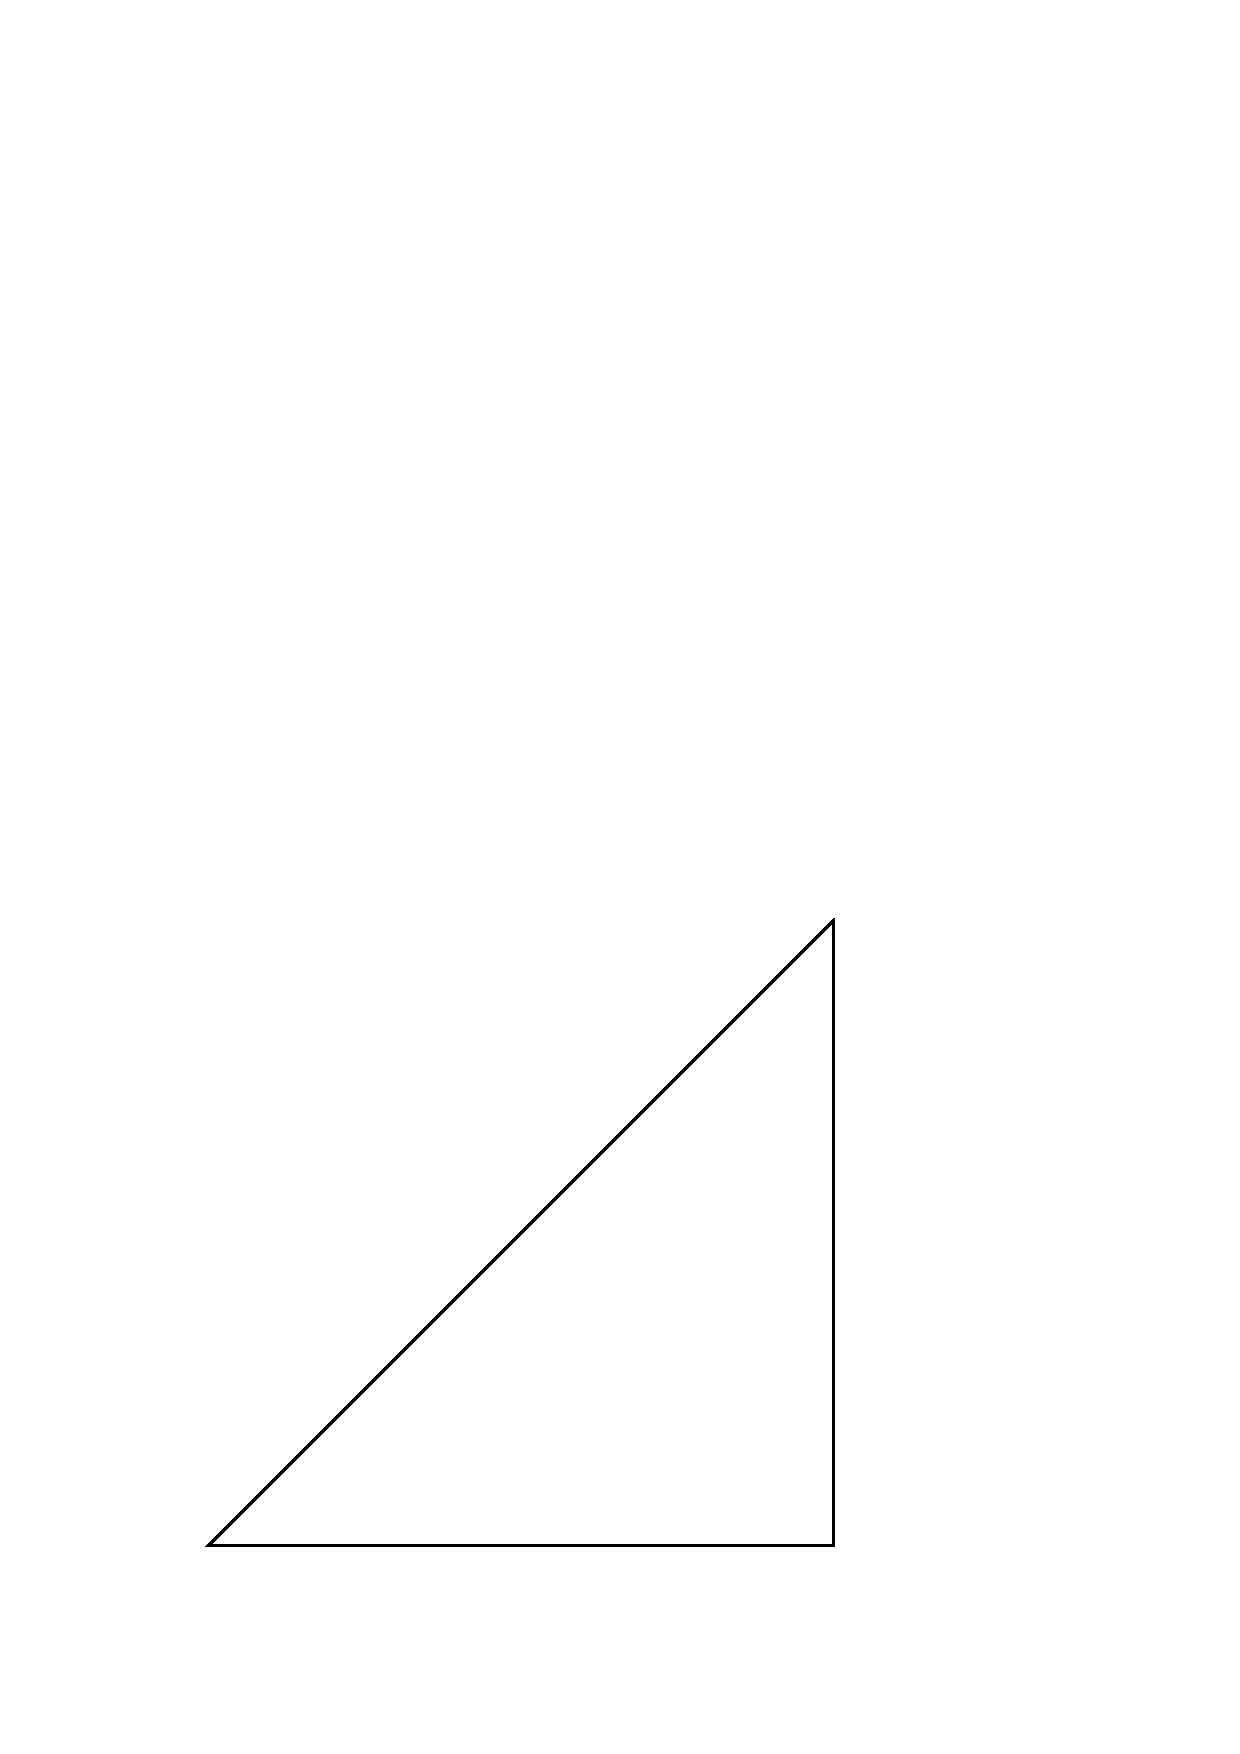
\includegraphics[natwidth=298,natheight=421,alt={A single line}]{manualimages/line.pdf}}
\else
\fbox{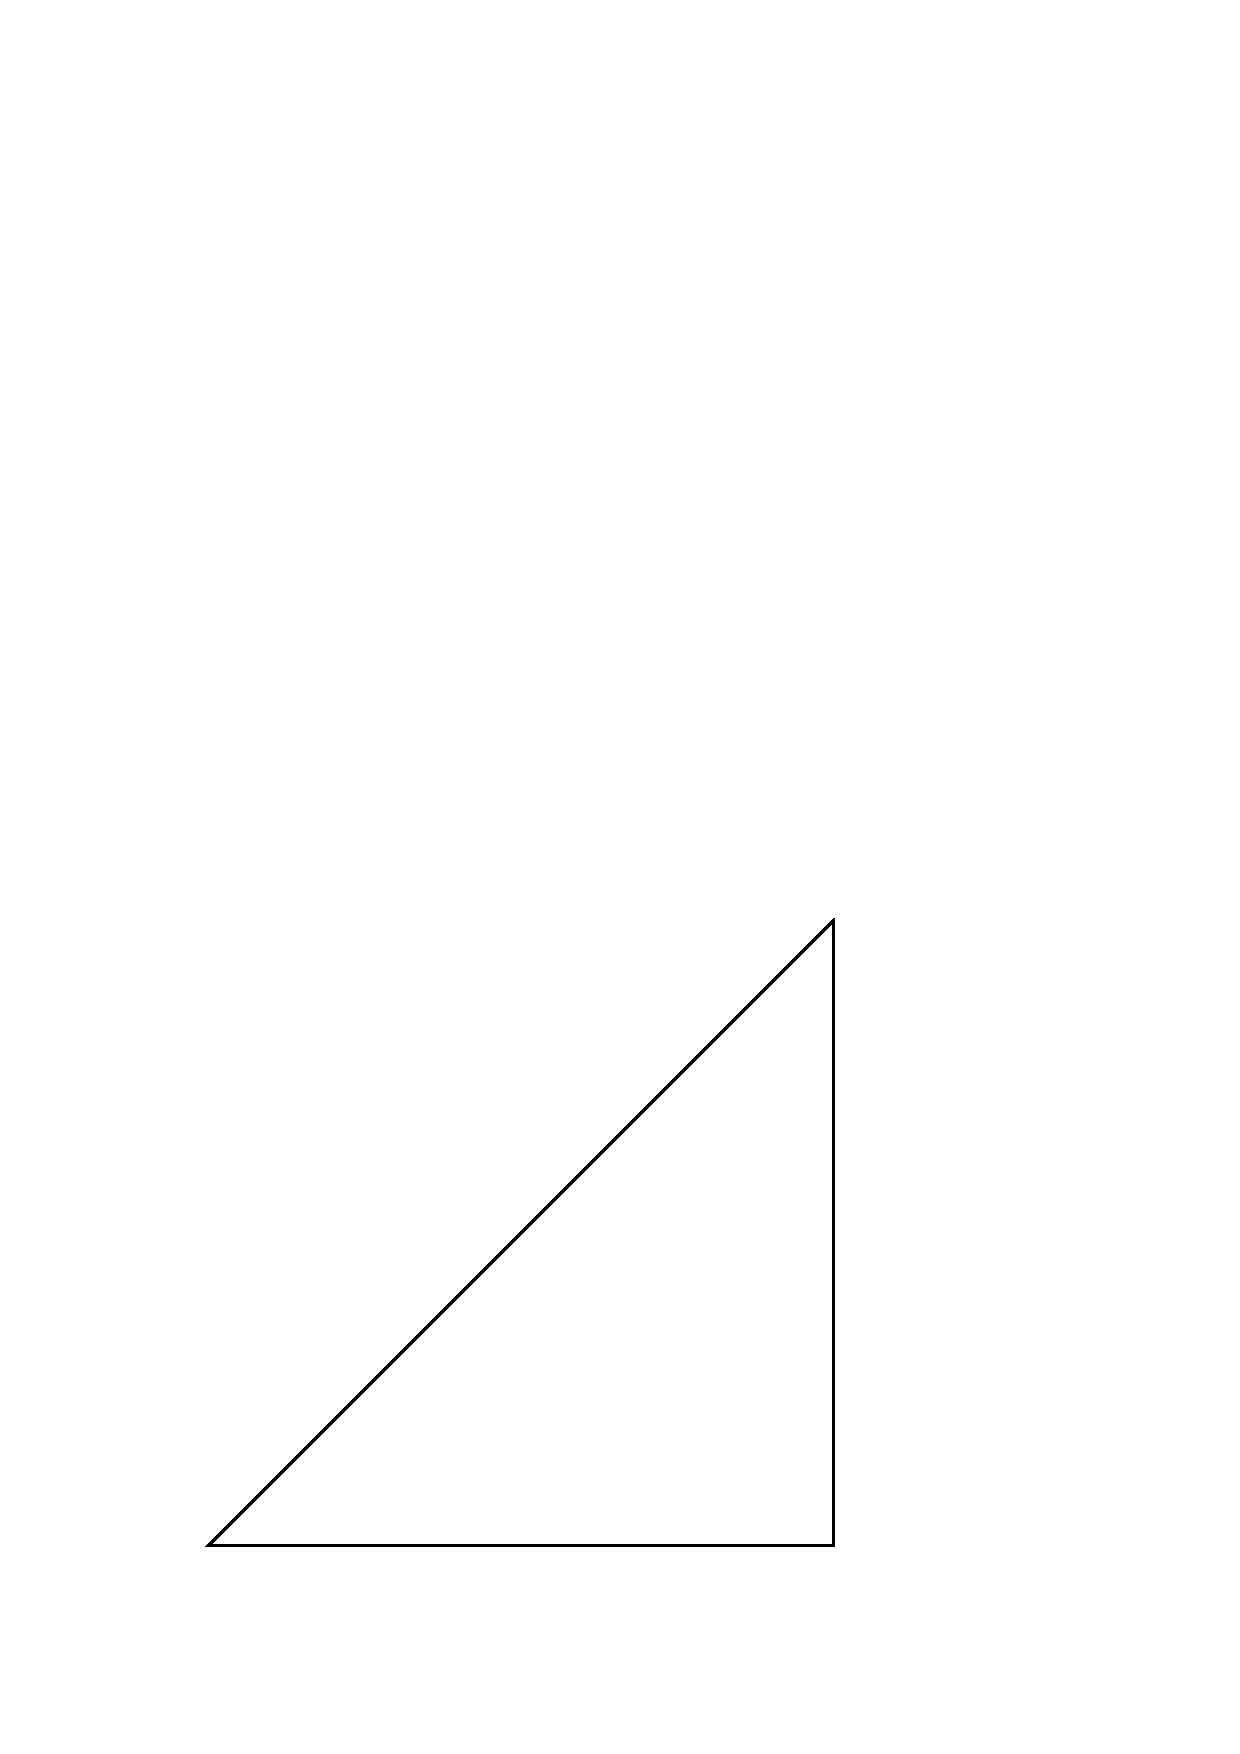
\includegraphics[width=0.3\textwidth,alt={A single line}]{manualimages/line.pdf}}
\fi
\bigskip

\noindent Alternatively, we may use \texttt{-close} to draw the final line back to the starting point:

\begin{framed}
 \noindent\small\verb?cpdf -create-pdf AND -draw -to "100 100" -line "400 400"?\\
 \noindent\small\verb?     -line "400 100" -close -stroke?\\
 \noindent\small\verb?     -o out.pdf?
\end{framed}

\noindent We can have multiple such subpaths in a path, by closing and carrying on. We can fill our path with \texttt{-fill}:

\begin{framed}
 \noindent\small\verb?cpdf -create-pdf AND -draw -to "100 100" -line "400 400"?\\
 \noindent\small\verb?     -line "400 100" -close -fill?\\
 \noindent\small\verb?     -o out.pdf?
\end{framed}

\noindent Now we have a filled triangle:

\bigskip
\ifdefined\HCode
\fbox{
\includegraphics[natwidth=298,natheight=421,alt={A filled triangle}]{manualimages/fill.pdf}}
\else
\fbox{
\includegraphics[width=0.3\textwidth,alt={A filled triangle}]{manualimages/fill.pdf}}
\fi
\bigskip

\noindent The operations \texttt{-filleo}, \texttt{-strokefill} and \texttt{-strokefilleo} provide alternative combinations of stroke, fill, and winding rule.

We can save time when drawing rectangles by using the \texttt{-rect} operation, which takes the lower left coordinate, width and height. There is no need to explicitly close the rectangle.

\begin{framed}
 \noindent\small\verb?cpdf -create-pdf AND -draw -rect "200 300 200 300" -stroke?\\
 \noindent\small\verb?     -o out.pdf?
\end{framed}

\noindent We can build bezier curves using \texttt{-bez}, \texttt{-bez23} and \texttt{-bez13}. The first adds a bezier path using six coordinates - for the control points first, and then for the end point (the start point is the current coordinate):

\begin{framed}
 \noindent\small\verb?cpdf -create-pdf AND -draw -to "100 100" -bez "400 600 600 400 300 300"?\\
 \noindent\small\verb?     -stroke -o out.pdf?
\end{framed}

\noindent Here is the result:

\bigskip
\ifdefined\HCode
\fbox{
\includegraphics[natwidth=298,natheight=421,alt={A bezier line}]{manualimages/bez.pdf}}
\else
\fbox{
\includegraphics[width=0.3\textwidth,alt={A bezier line}]{manualimages/bez.pdf}}
\fi
\bigskip

\noindent The operation \texttt{-bez23} is a shorthand used when the first control point is equal to the current point. The operation \texttt{-bez13} is a shorthand used when the second control point is equal to the final point.

To avoid calculating the Bezier curves for a circle manually, Cpdf can generate them automatically when given the centre and radius:

\begin{framed}
 \noindent\small\verb?cpdf -create-pdf AND -draw -circle "200 200 100"?\\
 \noindent\small\verb?     -stroke -o out.pdf?
\end{framed}

\section{Clipping with paths}
  {\small\begin{framed}
   \noindent\verb!-clip! Clip\\
   \noindent\verb!-clipeo! Clip, even odd
  \end{framed}}

\noindent We can use a path to form a clipping region for subsequent content using \texttt{-clip} or \texttt{-clipeo}. For example: 

\begin{framed}
 \noindent\small\verb?cpdf -create-pdf AND -draw -circle "300 300 100" -clip?\\
 \noindent\small\verb?     -circle "300 350 100" -fill -o out.pdf?
\end{framed}

\noindent Here is the result:

\bigskip
\ifdefined\HCode
\fbox{
\includegraphics[natwidth=298,natheight=421,alt={One circle clipped to another}]{manualimages/clip.pdf}}
\else
\fbox{
\includegraphics[width=0.3\textwidth,alt={One circle clipped to another}]{manualimages/clip.pdf}}
\fi
\bigskip

\section{Path parameters}
  {\small\begin{framed}
   \noindent\verb!-strokecol "g" | "r g b" | "c y m k" | <namedcolour>! Set stroke colour\\
   \noindent\verb!-fillcol "g" | "r g b" | "c y m k" | <namedcolour>! Set fill colour\\
   \noindent\verb!-thick <n>! Set stroke thickness\\
   \noindent\verb!-cap butt | round | square! Set cap\\
   \noindent\verb!-join miter | round | bevel! Set join\\
   \noindent\verb!-miter <n>! Set miter limit\\
   \noindent\verb!-dash <pattern>! Set dash pattern
  \end{framed}}

We can set stroke and fill colours for our paths, either as greyscale (one component), RGB (three components) or CMYK (four components), or by naming a colour as described in Chapter 8:

\begin{framed}
 \noindent\small\verb?cpdf -create-pdf AND -draw -circle "200 200 100" -thick 20?\\
 \noindent\small\verb?     -strokecol 0.5 -fillcol "0.2 0.7 0.2" -strokefill -o out.pdf?
\end{framed}

\noindent Here is the result:

\bigskip
\ifdefined\HCode
\fbox{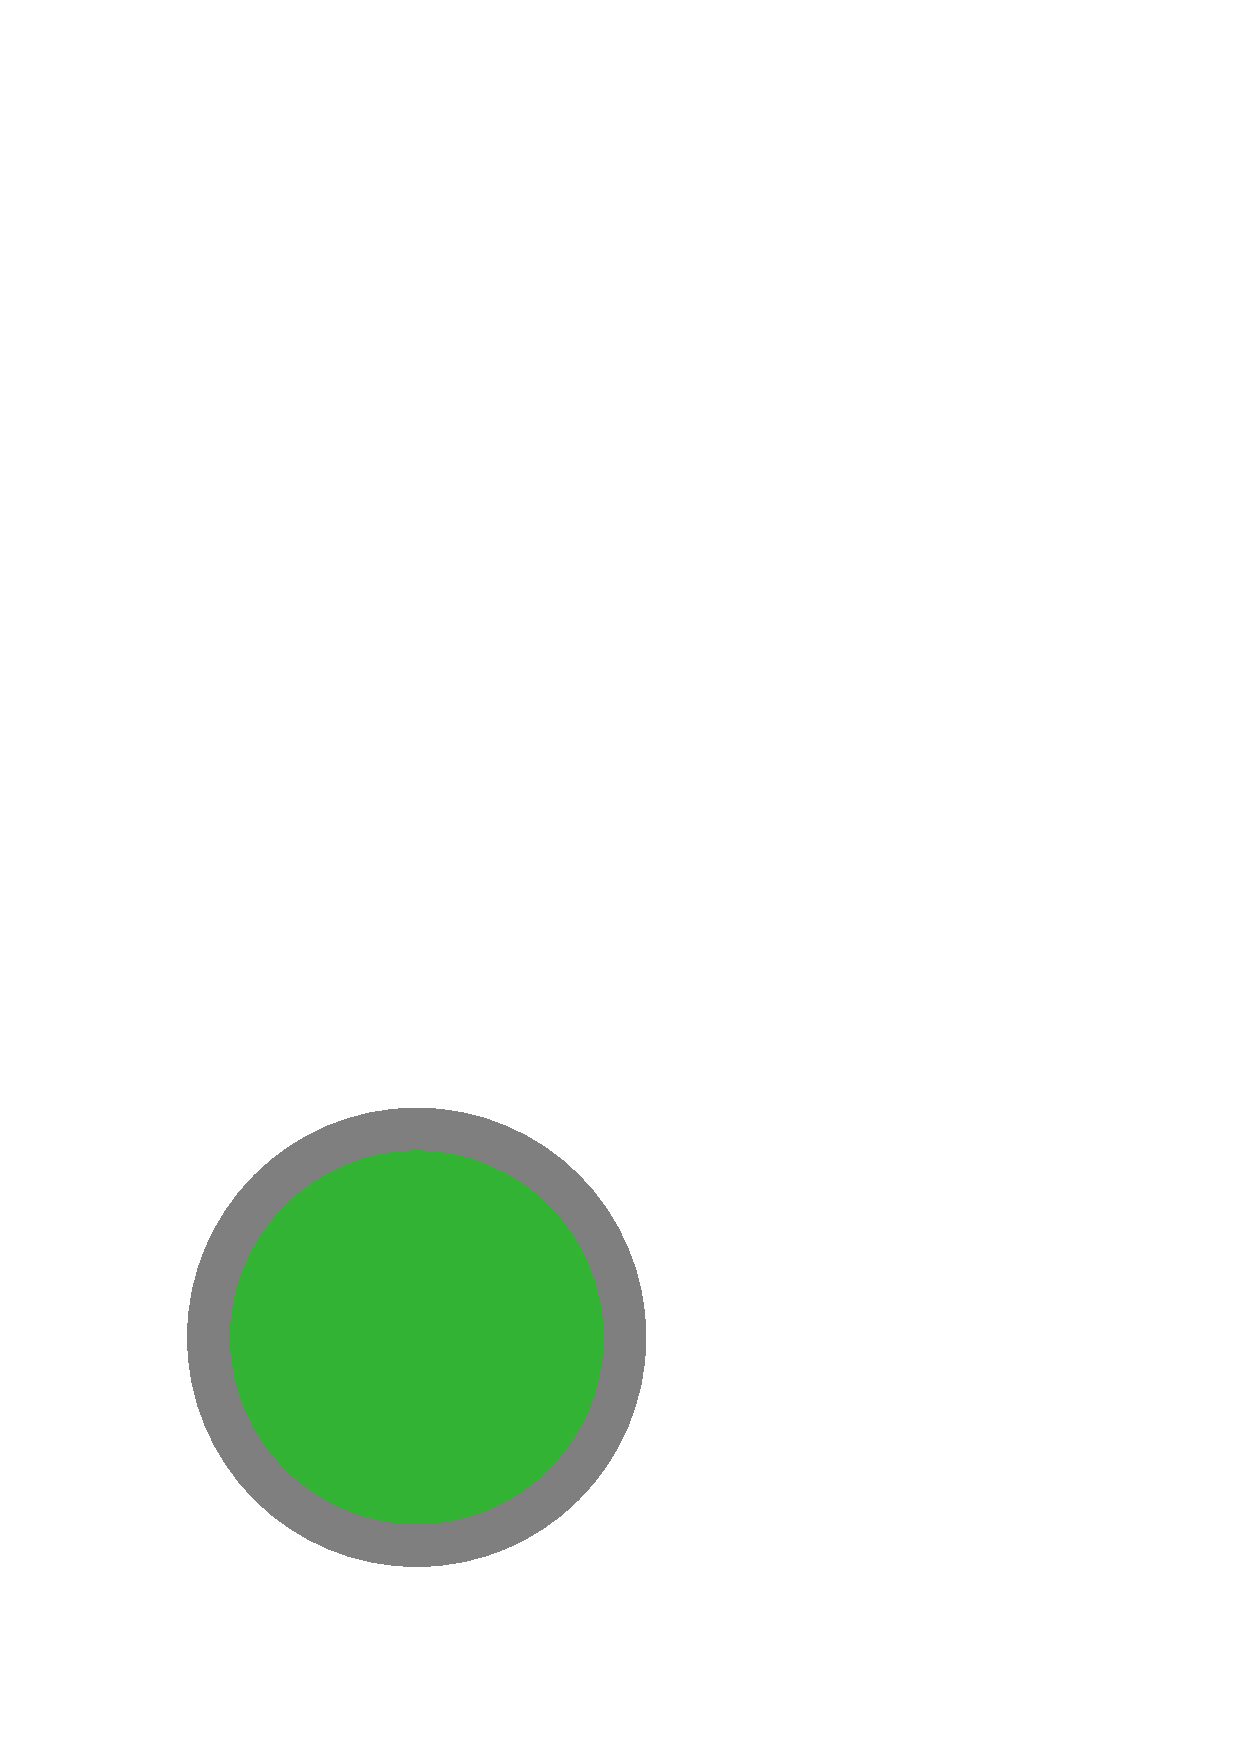
\includegraphics[natwidth=298,natheight=421,alt={Stroke and fill colours}]{manualimages/colfill.pdf}}
\else
\fbox{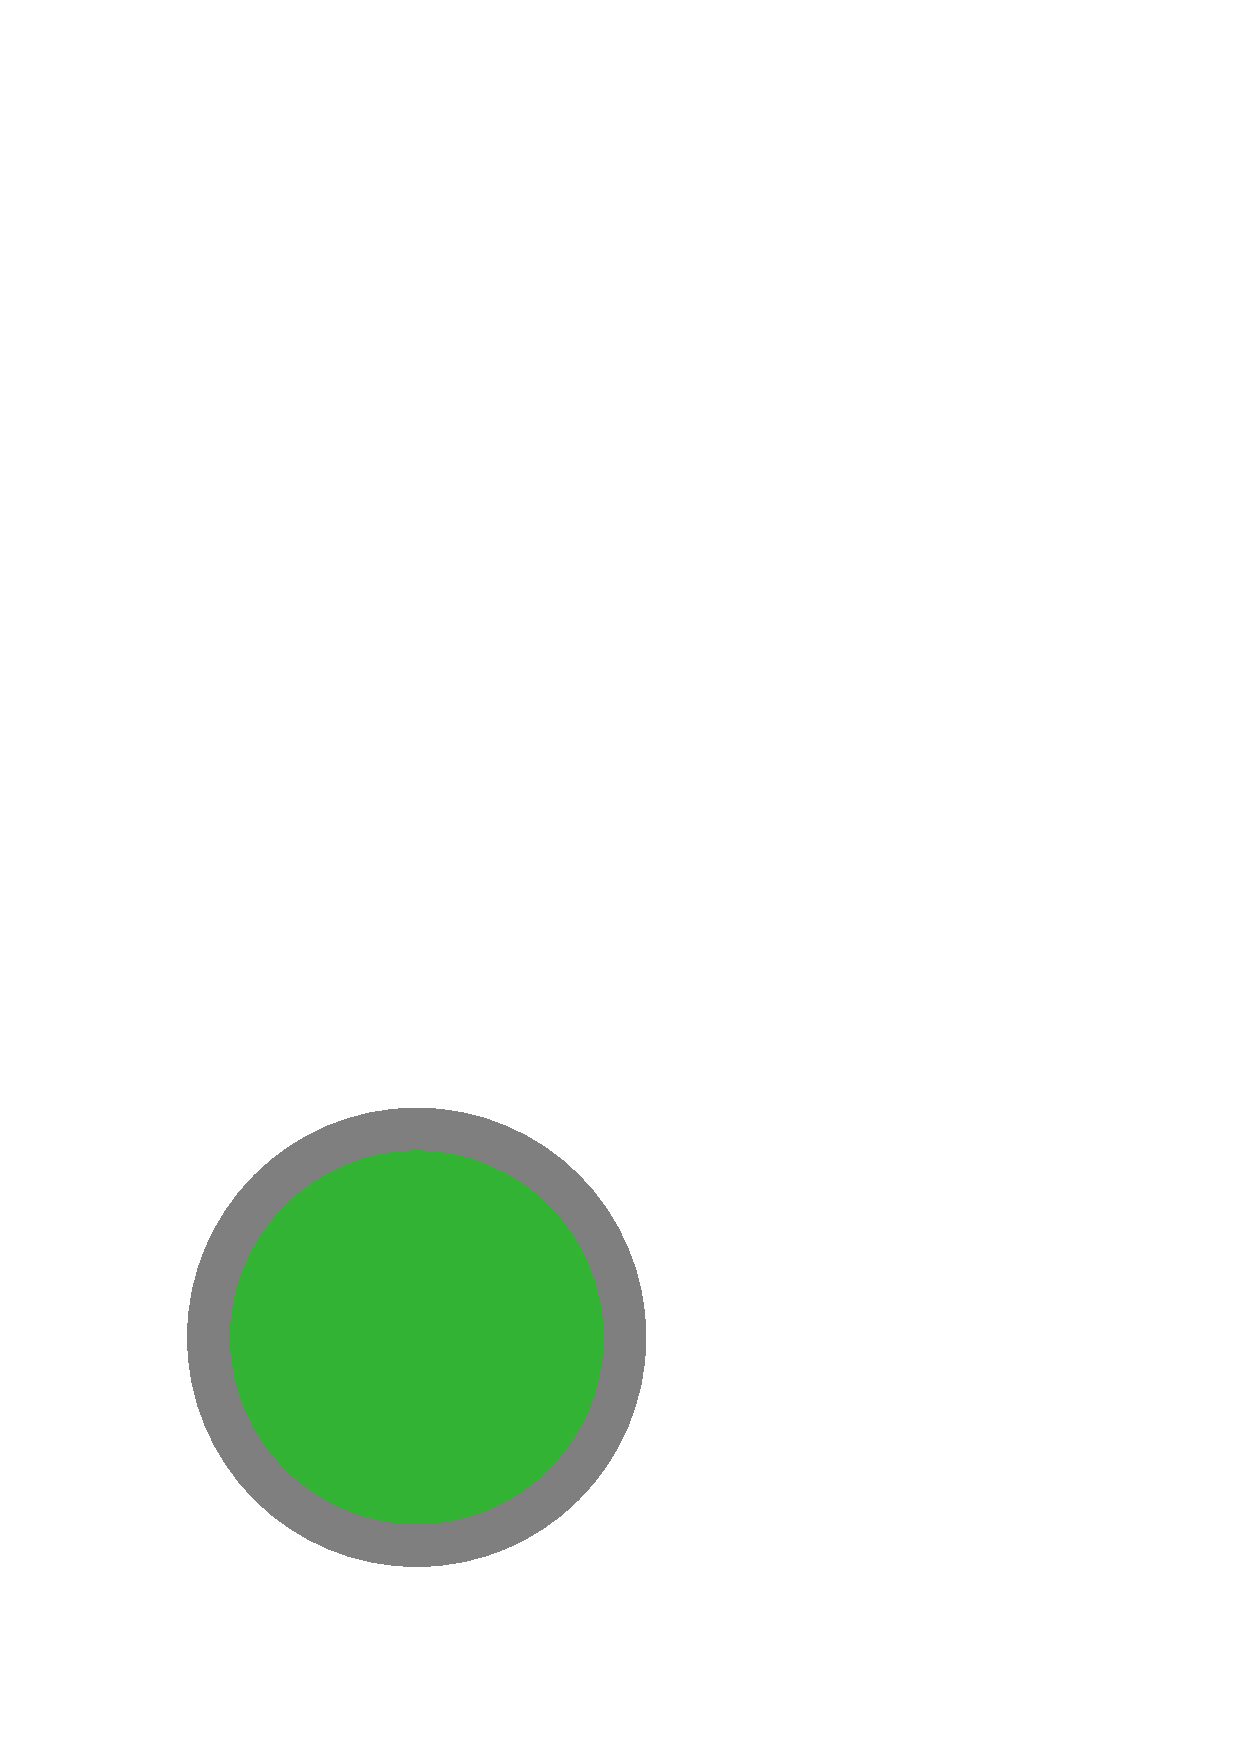
\includegraphics[width=0.3\textwidth,alt={Stroke and fill colours}]{manualimages/colfill.pdf}}
\fi
\bigskip

\noindent We can set line caps and joins with \texttt{-cap}, \texttt{-join}:

\begin{framed}
 \noindent\small\verb?cpdf -create-pdf AND -draw -to "100 100"?\\
 \noindent\small\verb?     -join round -cap round -thick 40?\\
 \noindent\small\verb?     -line "200 200" -line "220 100" -stroke?\\
 \noindent\small\verb?     -o out.pdf?
\end{framed}

\noindent Then we see:

\bigskip
\ifdefined\HCode
\fbox{
\includegraphics[natwidth=298,natheight=421,alt={Caps and joins}]{manualimages/capjoins.pdf}}
\else
\fbox{
\includegraphics[width=0.3\textwidth,alt={Caps and joins}]{manualimages/capjoins.pdf}}
\fi
\bigskip

\noindent The miter limit (see PDF reference for details) may be set with \texttt{-miter}.

Lines may have dash patterns. A dash pattern consists of one or more numbers. All save the last form the list of dash lengths and gap lengths. The last is the phase, which defines how far along the pattern we start. For example, using a dash pattern of "30 20 0" i.e black 30, white 20, phase 0:

\begin{framed}
 \noindent\small\verb?cpdf -create-pdf AND -draw -to "100 100"?\\
 \noindent\small\verb?     -dash "30 20 0" -thick 20 -line "400 300" -stroke?\\
 \noindent\small\verb?     -o out.pdf?
\end{framed}

\noindent Here is the result:

\bigskip
\ifdefined\HCode
\fbox{
\includegraphics[natwidth=298,natheight=421,alt={Dash patterns}]{manualimages/dash.pdf}}
\else
\fbox{
\includegraphics[width=0.3\textwidth,alt={Dash patterns}]{manualimages/dash.pdf}}
\fi
\bigskip

\section{The graphics stack and matrices}
  {\small\begin{framed}
   \noindent\verb!-push! Push graphics stack\\
   \noindent\verb!-pop! Pop graphics stack\\
   \noindent\verb!-matrix "a b c d e f"! Append to graphics matrix\\
   \noindent\verb!-mtrans "tx ty"! Translate the graphics matrix\\
   \noindent\verb!-mrot "x y a"! Rotate the graphics matrix counterclockwise around \texttt{(x, y)} by angle \texttt{a} in radians\\
   \noindent\verb!-mscale "x y sx sy"! Scale the graphics matrix around \texttt{(x, y)}\\
   \noindent\verb!-mshearx "x y a"! Shear the graphics matrix in X around \texttt{(x, y)} by angle \texttt{a}\\
   \noindent\verb!-msheary "x y a"! Shear the graphics matrix in Y around \texttt{(x, y)} by angle \texttt{a}
  \end{framed}}

PDF maintains a stack of graphics state, which we can manipulate with \texttt{-push} which stores the current state, then modify the state for our own purposes, and then use \texttt{-pop} to restore the previous state. Such invocations may be nested. Here is a simple example:
 
\begin{framed}
 \noindent\small\verb?cpdf -create-pdf AND -draw -circle "200 200 100" -fillcol red -fill?\\
 \noindent\small\verb?     -push -fillcol blue -circle "300 300 100" -fill?\\
 \noindent\small\verb?     -pop -circle "400 400 100" -fill  -o out.pdf?
\end{framed}

\noindent When we use \texttt{-pop} the colour returns to the saved one:

\bigskip
\ifdefined\HCode
\fbox{
\includegraphics[natwidth=298,natheight=421,alt={Push and pop}]{manualimages/pop.pdf}}
\else
\fbox{
\includegraphics[width=0.3\textwidth,alt={Push and pop}]{manualimages/pop.pdf}}
\fi
\bigskip

\noindent One very common use for a \texttt{-push}/\texttt{-pop} pair is to isolate the effects of an operation which modifies the current transformation matrix. These operations are used to translate, rotate, scale and so on. For example: 

\begin{framed}
 \noindent\small\verb?cpdf -create-pdf AND -draw -circle "200 200 100" -stroke -push?\\
 \noindent\small\verb?     -mrot "0 0 -0.3" -mscale "0 0 1.5 2" -circle "200 200 100" -stroke?\\
 \noindent\small\verb?     -pop -circle "200 200 50" -fill -o out.pdf?
\end{framed}

\noindent This is the result. See how the graphics transformation is undone when \texttt{-push} is invoked:

\bigskip
\ifdefined\HCode
\fbox{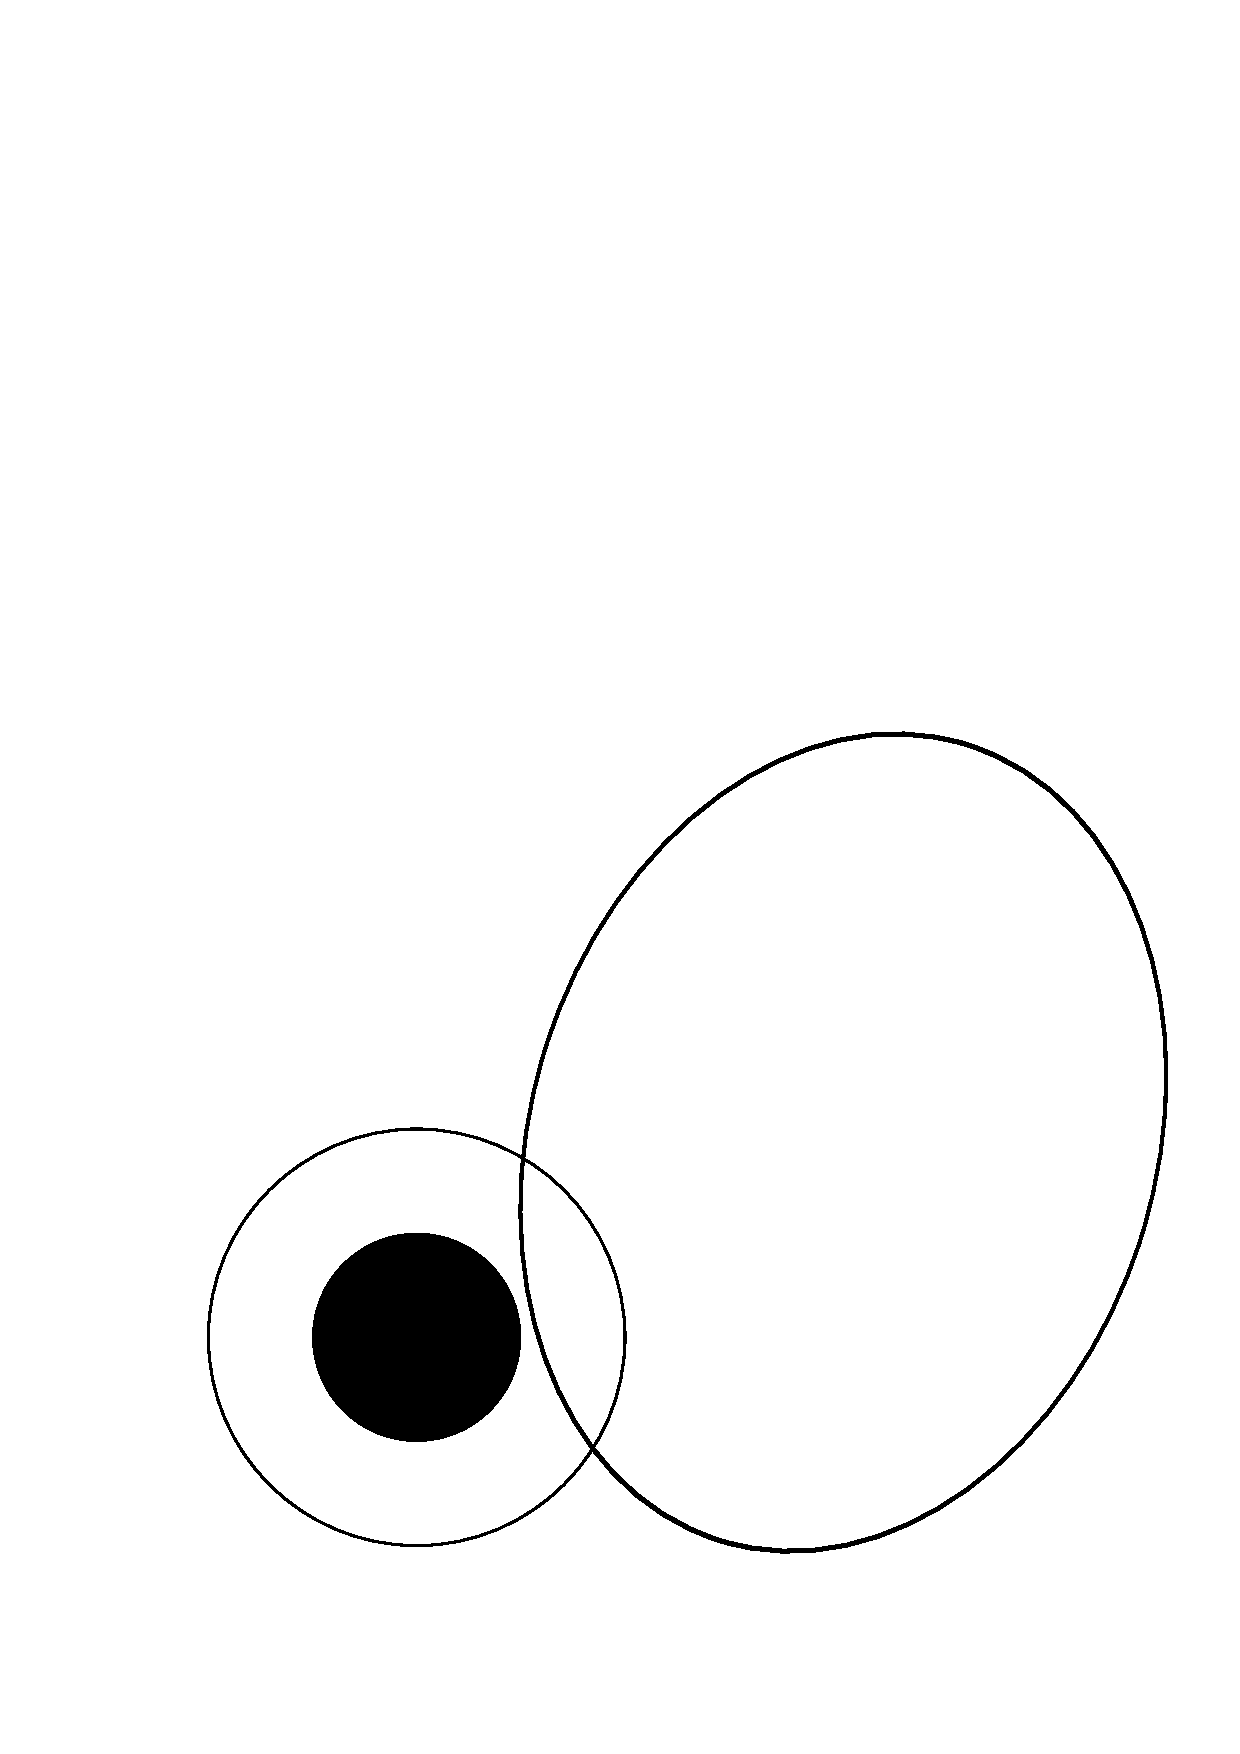
\includegraphics[natwidth=298,natheight=421,alt={Altering the graphics matrix}]{manualimages/matrix.pdf}}
\else
\fbox{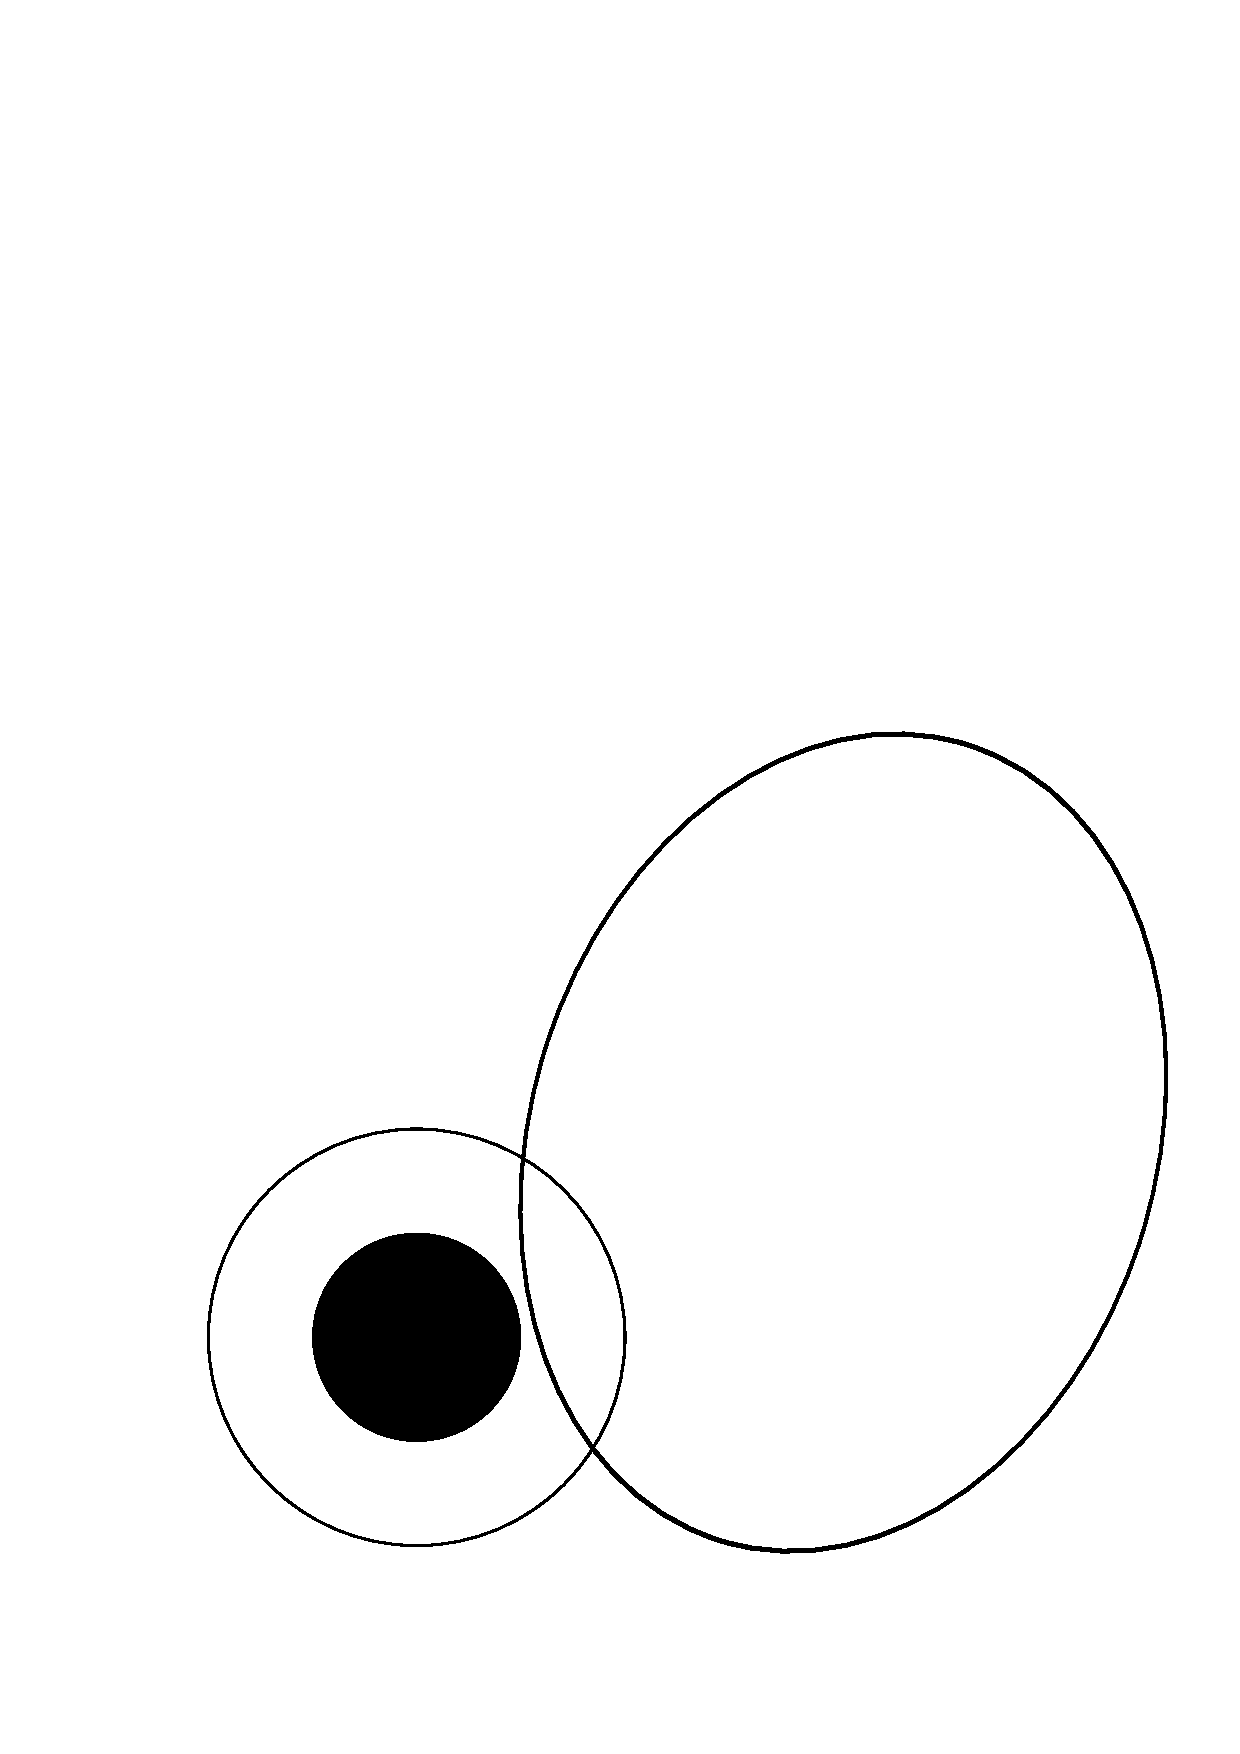
\includegraphics[width=0.3\textwidth,alt={Altering the graphics matrix}]{manualimages/matrix.pdf}}
\fi
\bigskip

\noindent This is important because, in the absence of \texttt{-push} and \texttt{-pop} there would be no way to reverse the effect of a graphics matrix modification except to manually calculate its inverse and apply it.

NB: When writing text (see below) the \texttt{-font} option is not subject to \texttt{-push} and \texttt{-pop}. Text is set the the font most recently chosen on the command line.

\section{Re-use with XObjects}

  {\small\begin{framed}
   \vspace{1.5mm}
   \noindent\verb!-xobj-bbox "x y w h"! Specify the bounding box for xobjects\\
   \noindent\verb!-xobj <name>! Begin saving a sequence of graphics operators\\
   \noindent\verb!-end-xobj! End saving a sequence of graphics operators\\
   \noindent\verb!-use <name>! Use a saved sequence of graphics operators
  \end{framed}}

In our examples, we have sometimes had to write the same operations multiple times. To avoid this, PDF has a mechanism called an XObject. This allows us to save a set of operations for re-use in different contexts, or on different pages. For example, here we store an XObject which just strokes a circle. We then \texttt{-use} it once, and alter the colour and transformation matrix and \texttt{-use} it again.

\begin{framed}
 \noindent\small\verb?cpdf -create-pdf AND -draw -xobj-bbox "0 0 200 200" -xobj A?\\
 \noindent\small\verb?     -circle "100 100 50" -stroke -end-xobj?\\
 \noindent\small\verb?     -use A -strokecol red -mtrans "20 20" -use A -o out.pdf?
\end{framed}

\noindent Note that we must specify a bounding box for the XObject with \texttt{-xobj-bbox}. Here is the result:

\bigskip
\ifdefined\HCode
\fbox{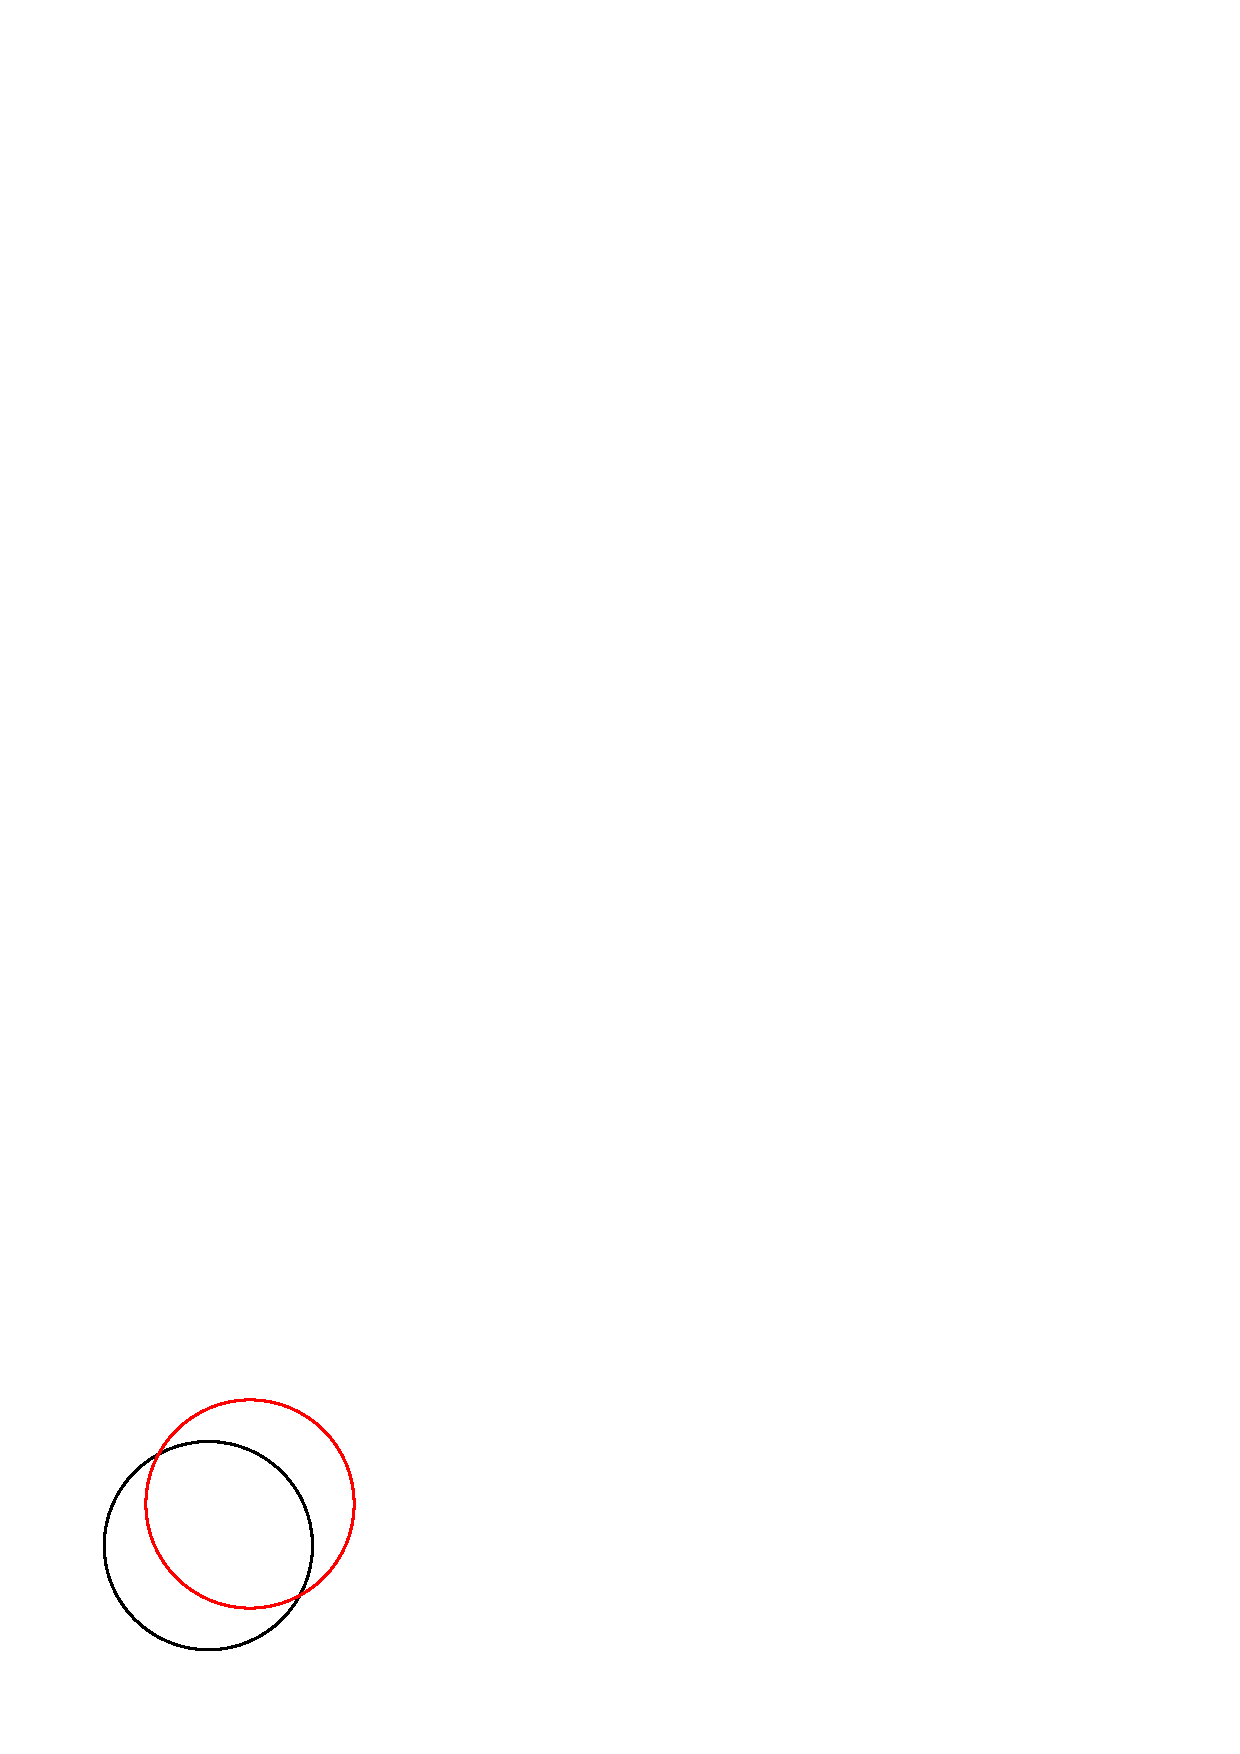
\includegraphics[natwidth=298,natheight=421,alt={An Xobject}]{manualimages/xobj.pdf}}
\else
\fbox{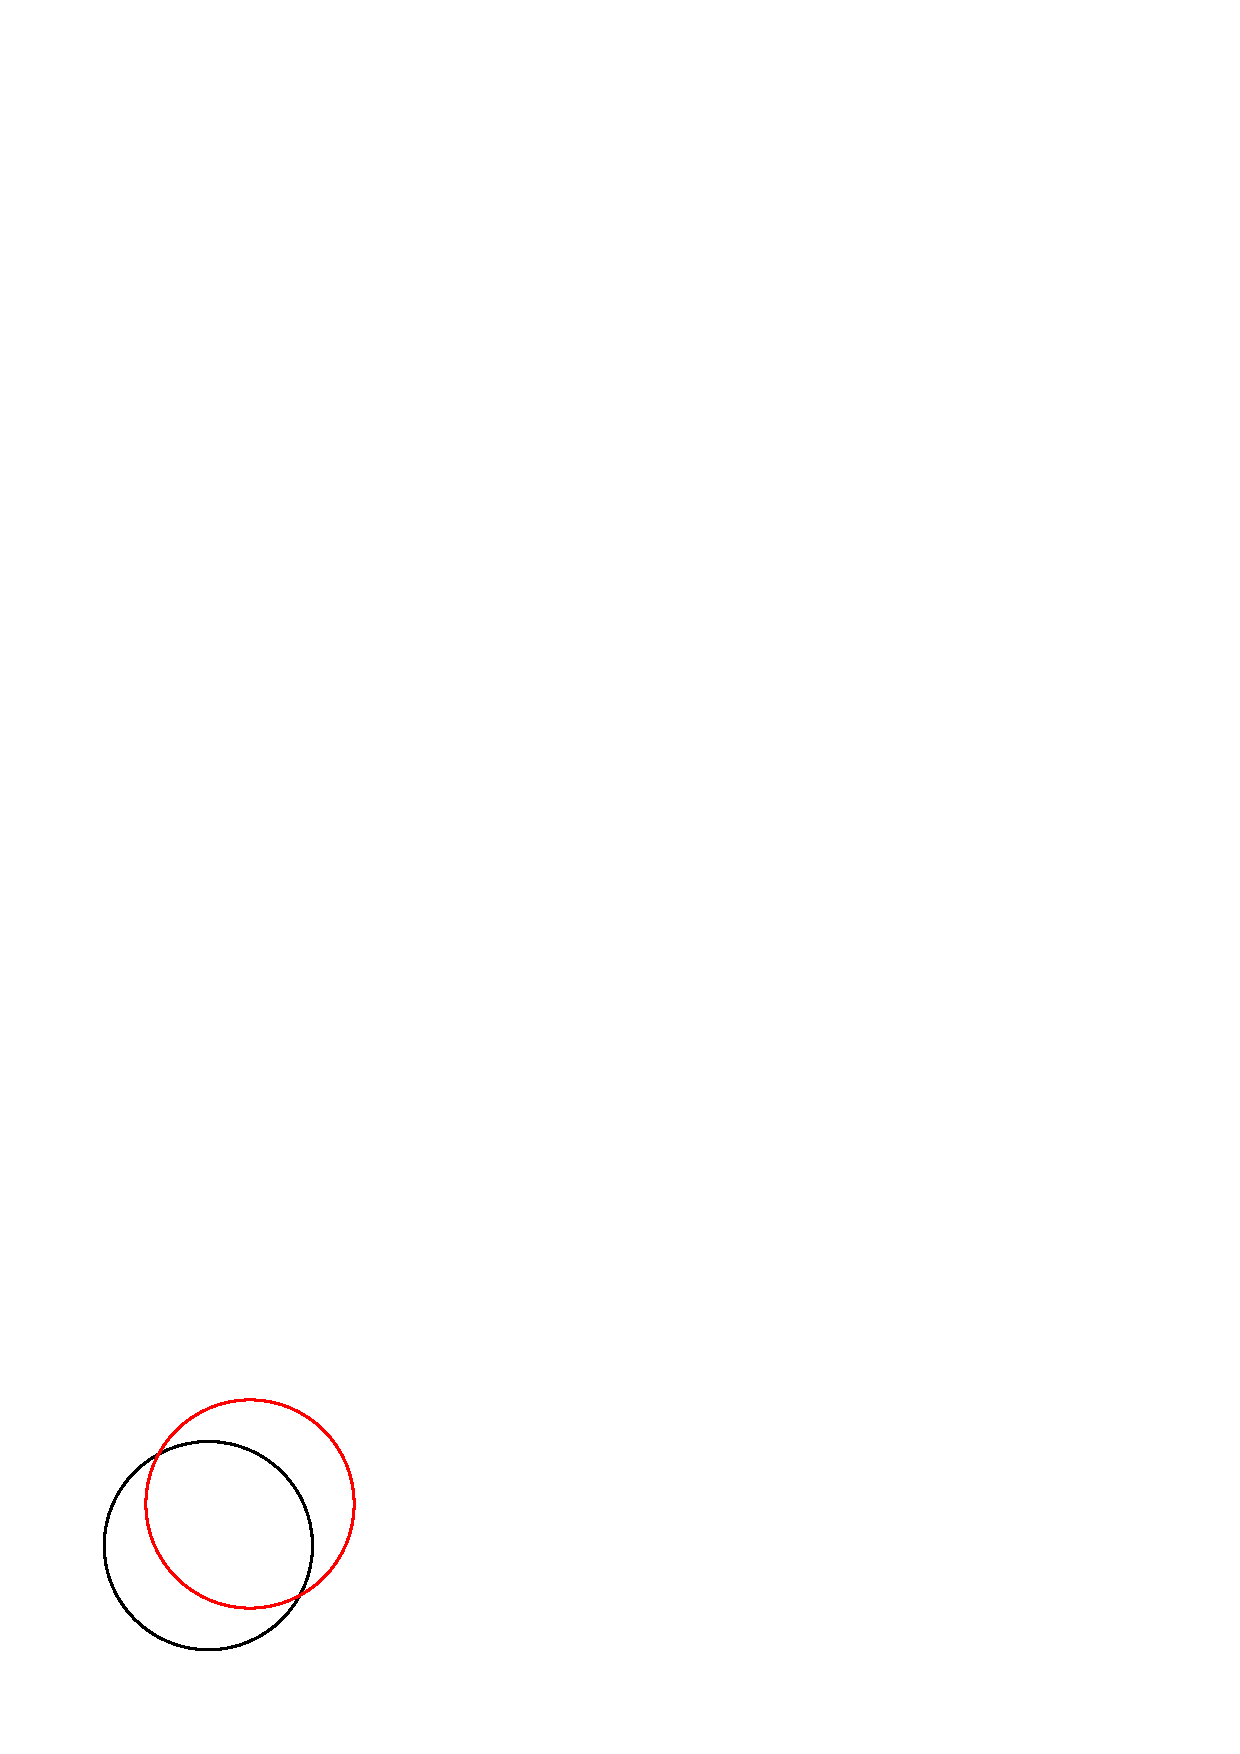
\includegraphics[width=0.3\textwidth,alt={An XObject}]{manualimages/xobj.pdf}}
\fi
\bigskip

\noindent XObjects may be nested.

\section{Images}
  {\small\begin{framed}
   \noindent\verb!-draw-jpeg <name>=<filename>! Load a JPEG from file and name it\\
   \noindent\verb!-draw-png <name>=<filename>! Load a PNG from file and name it\\
   \noindent\verb!-image <name>! Draw an image which has already been loaded
  \end{framed}}

We can include a 24bit non-transparent and non-interlaced PNG, or any JPEG by using \texttt{-draw-jpeg} or \texttt{-draw-png} to load it and assign it a name. We can then use \texttt{-image} to use it at any point:

\begin{framed}
 \noindent\small\verb?cpdf -create-pdf AND -draw -draw-png A=sheet.png?\\
 \noindent\small\verb?     -mscale "0 0 400 294" -image A -o out.pdf?
\end{framed}

\noindent Here is the result:

\bigskip
\ifdefined\HCode
\fbox{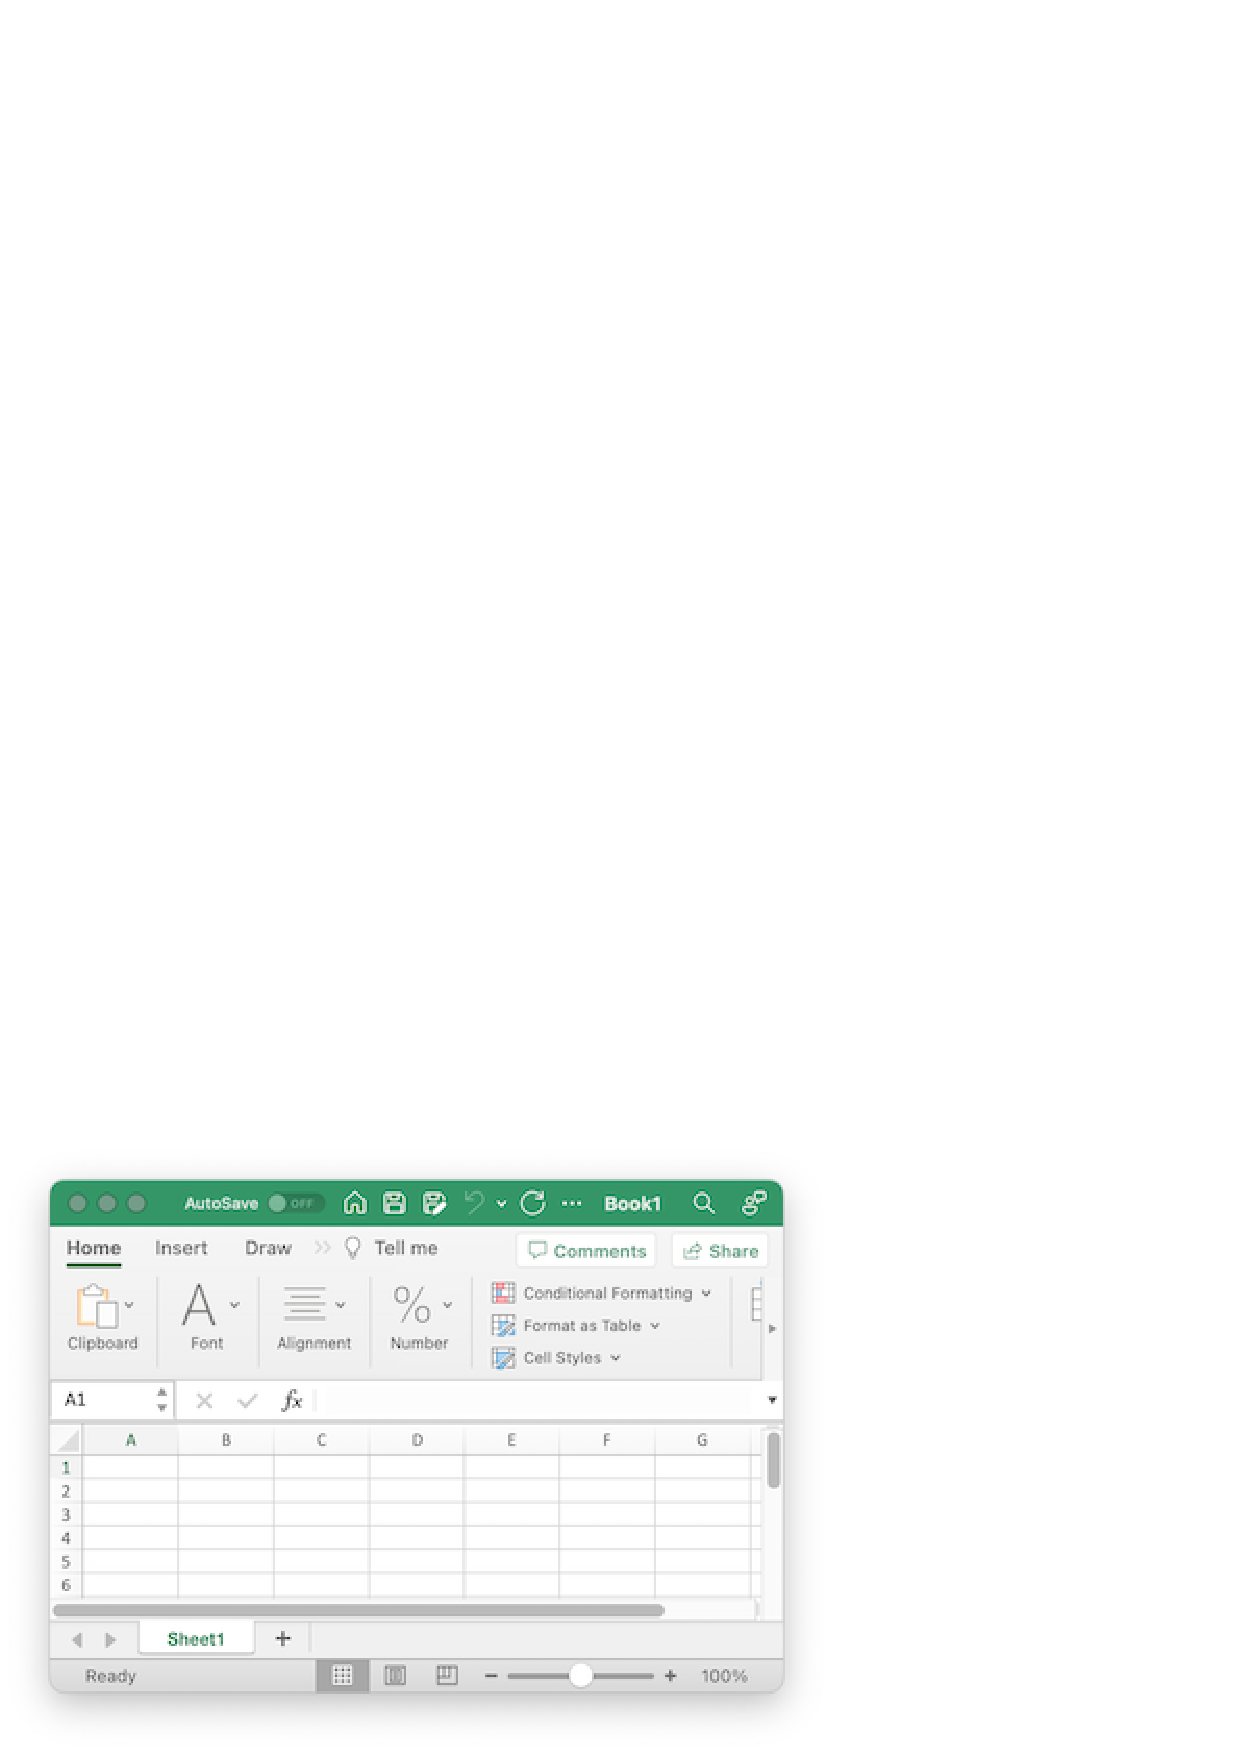
\includegraphics[natwidth=298,natheight=421,alt={Drawing a PNG on a PDF}]{manualimages/png.pdf}}
\else
\fbox{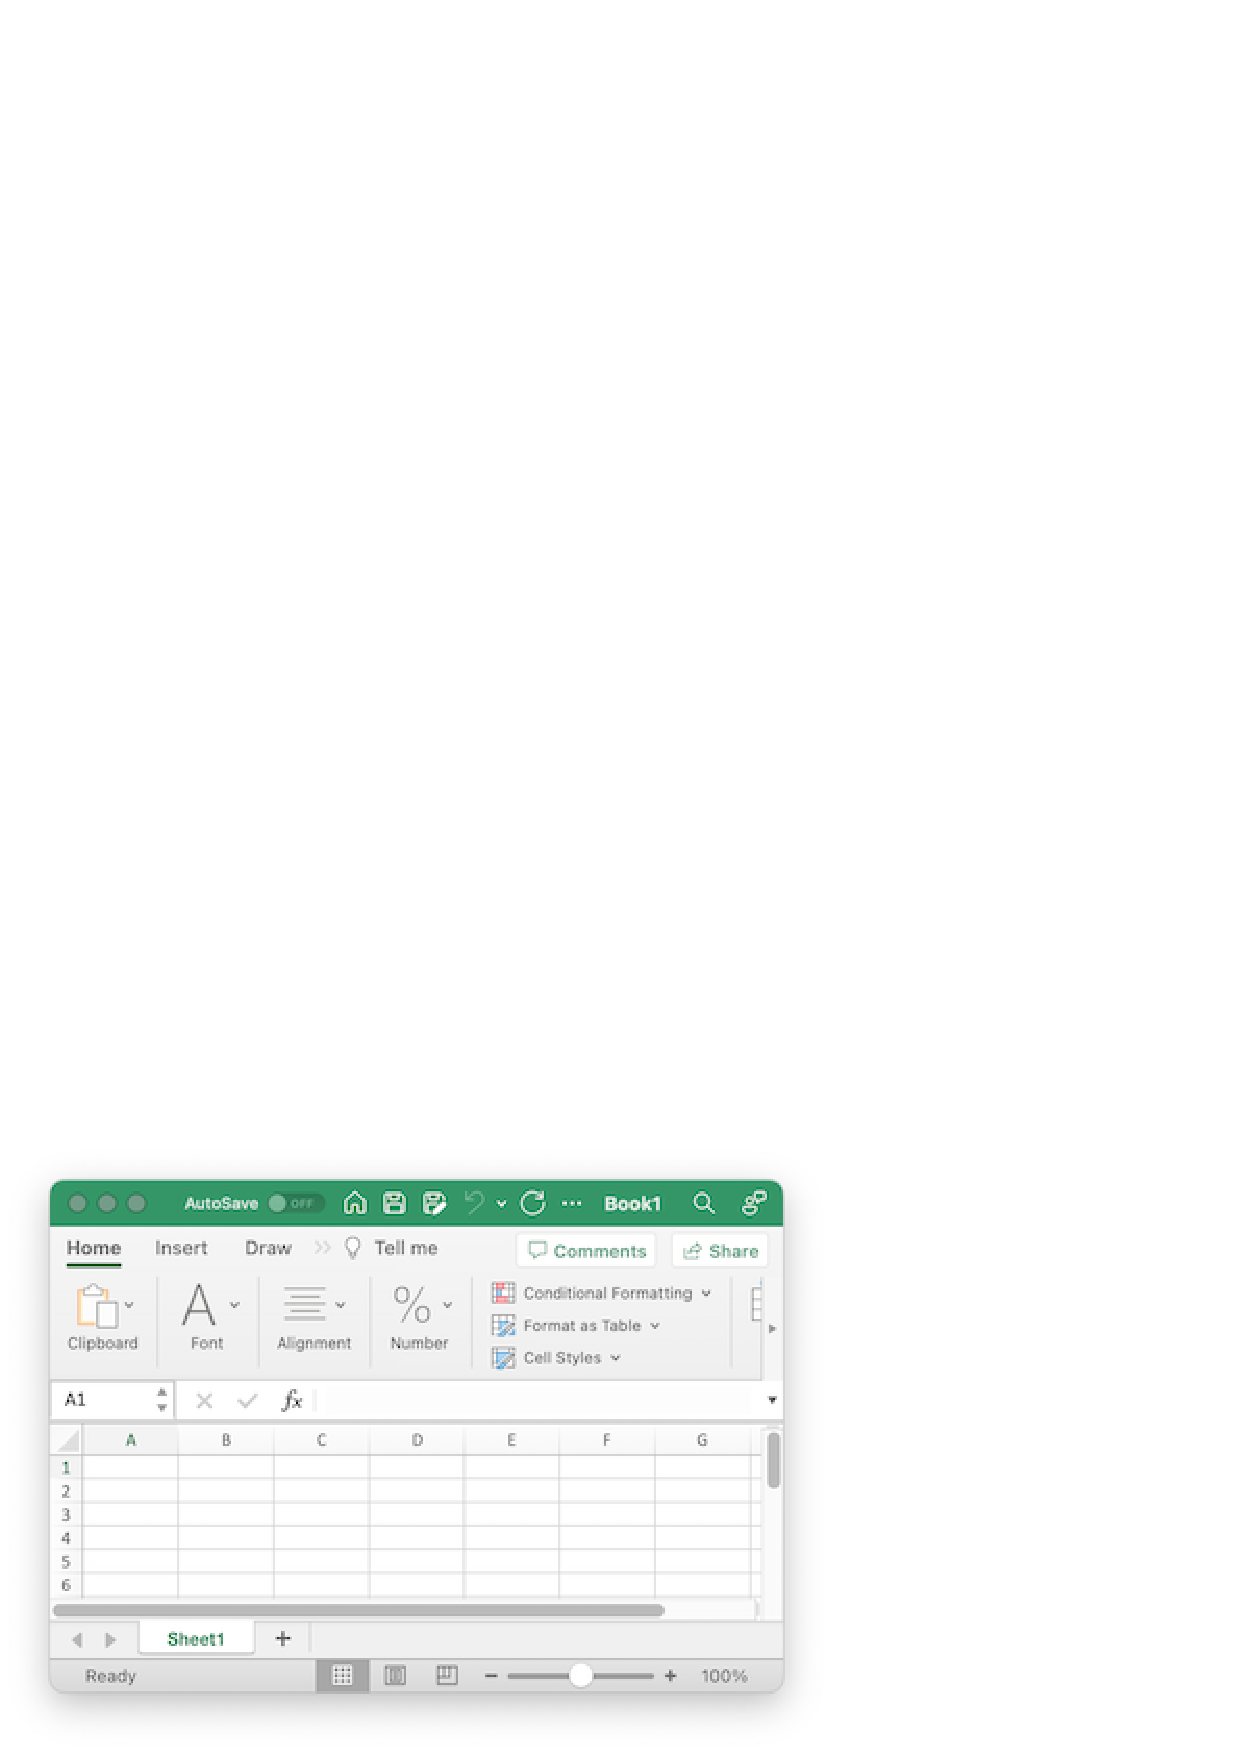
\includegraphics[width=0.3\textwidth,alt={Drawing a PNG on a PDF}]{manualimages/png.pdf}}
\fi
\bigskip

\noindent You can see we had to scale by the width and height of the image to draw it at the size we expect.

\section{Transparency}
  {\small\begin{framed}
   \noindent\verb!-fill-opacity <n>! Set opacity\\
   \noindent\verb!-stroke-opacity <n>! Set stroke opacity
  \end{framed}}

We can set fill and stroke transparencies, between 0 (fully transparent) and 1 (fully opaque):

\begin{framed}
 \noindent\small\verb?cpdf -create-pdf AND -draw -fill-opacity 0.5?\\
 \noindent\small\verb?     -circle "250 300 150" -fill -circle "350 300 150" -fill?\\
 \noindent\small\verb?     -o out.pdf?
\end{framed}

\noindent Here is the result:

\bigskip
\ifdefined\HCode
\fbox{
\includegraphics[natwidth=298,natheight=421,alt={Fill and stroke transparency}]{manualimages/trans.pdf}}
\else
\fbox{
\includegraphics[width=0.3\textwidth,alt={Fill and stroke transparency}]{manualimages/trans.pdf}}
\fi
\bigskip

\noindent Notice that we used \texttt{-fill} twice, to ensure each circle was in a different path. If they had been part of the same path, the effect would be different.


\section{Text}

  {\small\begin{framed}
   \noindent\verb!-bt! Begin text\\
   \noindent\verb!-et! End text\\
   \noindent\verb!-text <text>! Draw text\\
   \noindent\verb!-stext <text>! Draw text with \%specials\\
   \noindent\verb!-font <fontname>! Set font\\
   \noindent\verb!-font-size <n>! Set font size\\
   \noindent\verb!-leading <n>! Set leading\\
   \noindent\verb!-charspace <n>! Set character spacing\\
   \noindent\verb!-wordspace <n>! Set word space\\
   \noindent\verb!-textscale <n>! Set text scale\\
   \noindent\verb!-rendermode <n>! Set text rendering mode\\
   \noindent\verb!-rise <n>! Set text rise\\
   \noindent\verb!-nl! New line\end{framed}}

We can draw text in a \textit{text section}, which must start with \texttt{-bt} and end with \texttt{-et}. For example:

\begin{framed}
 \noindent\small\verb?cpdf -create-pdf AND -draw -mtrans "50 50" -font Helvetica -font-size 144?\\
 \noindent\small\verb?     -bt -text "Hello" -et -o out.pdf?
\end{framed}

\noindent Here is the result:

\bigskip
\ifdefined\HCode
\fbox{
\includegraphics[natwidth=298,natheight=421,alt={Drawing text}]{manualimages/text.pdf}}
\else
\fbox{
\includegraphics[width=0.3\textwidth,alt={Drawing text}]{manualimages/text.pdf}}
\fi
\bigskip

\noindent If we use \texttt{-stext} instead of \texttt{-text} the usual special values from Chapter 8 (with the exception of URL links) may be used:

\begin{framed}
 \noindent\small\verb?cpdf -create-pdf AND -draw -mtrans "50 50" -font-size 144?\\
 \noindent\small\verb?     -bt -stext "Page %Page" -et -o out.pdf?
\end{framed}

\noindent Now we see:

\bigskip
\ifdefined\HCode
\fbox{
\includegraphics[natwidth=298,natheight=421,alt={Using special text}]{manualimages/stext.pdf}}
\else
\fbox{
\includegraphics[width=0.3\textwidth,alt={Using special text}]{manualimages/stext.pdf}}
\fi
\bigskip

\noindent We can use \texttt{-text} multiple times, interspersing operators which change the text state, such as font and font size:

\begin{framed}
 \noindent\small\verb?cpdf -create-pdf AND -draw -mtrans "10 20" -font-size 72?\\
 \noindent\small\verb?     -bt -text "Different " -font Times-BoldItalic -text "fonts"?\\
 \noindent\small\verb?     -font-size 36 -text " and sizes" -et -o out.pdf?
\end{framed}

\noindent Here is the result:

\bigskip
\ifdefined\HCode
\fbox{
\includegraphics[natwidth=298,natheight=421,alt={Font and font size}]{manualimages/fonts.pdf}}
\else
\fbox{
\includegraphics[width=0.3\textwidth,alt={Font and font size}]{manualimages/fonts.pdf}}
\fi
\bigskip

\noindent We can alter the character space, word space, horizontal scaling (100 = no scaling, less than 100 shrink, more than 100 stretch), and text rise:

\begin{framed}
 \noindent\small\verb?cpdf -create-pdf AND -draw -mtrans "10 20" -font-size 72?\\
 \noindent\small\verb?     -bt -textscale 75 -charspace 5 -wordspace 20 -text "Different "?\\
 \noindent\small\verb?     -font Times-BoldItalic -text "fonts" -font-size 36 -rise 40?\\
 \noindent\small\verb?     -text " and sizes" -et -o out.pdf? 
\end{framed}

\noindent Now we see:

\bigskip
\ifdefined\HCode
\fbox{
\includegraphics[natwidth=298,natheight=421,alt={Font parameters}]{manualimages/fontparams.pdf}}
\else
\fbox{
\includegraphics[width=0.3\textwidth,alt={Font parameters}]{manualimages/fontparams.pdf}}
\fi
\bigskip

\noindent Text may appear on multiple lines. We set up the line spacing with \texttt{-leading} then make new lines with \texttt{-nl}:

\begin{framed}
 \noindent\small\verb?cpdf -create-pdf AND -draw -mtrans "100 200" -font-size 50?\\
 \noindent\small\verb?     -leading 55 -bt -text "This is" -nl -text "on multiple"?\\
 \noindent\small\verb?     -nl -text "lines" -et -o out.pdf?
\end{framed}

\noindent Now we have:

\bigskip
\ifdefined\HCode
\fbox{
\includegraphics[natwidth=298,natheight=421,alt={Text on multiple lines}]{manualimages/lines.pdf}}
\else
\fbox{
\includegraphics[width=0.3\textwidth,alt={Text on multiple lines}]{manualimages/lines.pdf}}
\fi
\bigskip

\noindent When composing text, we may need to find the width of a piece of text to see where to break it, or for right alignment. We can use \texttt{-text-width} for this:

\begin{framed}
 \noindent\small\verb?cpdf -font Times-Roman -font-size 20 -text-width "Hello"?
\end{framed}

\noindent The result is in points.

We can change the text rendering mode to show outline text or, in this example, to use text as a clipping region:

\begin{framed}
 \noindent\small\verb?cpdf -create-pdf AND -draw -rendermode 7 -mtrans "100 200" -font-size 50?\\
 \noindent\small\verb?     -leading 55 -bt -text "This is" -nl -text "on multiple"?\\
 \noindent\small\verb?     -nl -text "lines" -et -circle "100 0 100" -fill -o out.pdf?
\end{framed}

\noindent Here is the result:

\bigskip
\ifdefined\HCode
\fbox{
\includegraphics[natwidth=298,natheight=421,alt={Clipping to text}]{manualimages/textclip.pdf}}
\else
\fbox{
\includegraphics[width=0.3\textwidth,alt={Clipping to text}]{manualimages/textclip.pdf}}
\fi
\bigskip


\noindent Here are the text rendering modes:

\bigskip
\begin{tabular}{lll}
  0&Fill text (default)&\\
  1&Stroke text&\\
  2&Fill, then stroke text&\\
  3&Neither fill nor stroke (invisible)&\\
  4&Fill text and add to path for clipping&\\
  5&Stroke text and add to path for clipping&\\
  6&Fill, then stroke text and add to path for clipping&\\
  7&Add text to path for clipping&
\end{tabular}
\bigskip

NB: When writing text the \texttt{-font} option is not subject to \texttt{-push} and \texttt{-pop}. Text is set the the font most recently chosen on the command line.

NB: To use a TrueType font with \texttt{-draw}, the \texttt{-load-ttf} must appear after the \texttt{-draw}.

NB: To use \texttt{-embed-std14}, put it before \texttt{-draw}.

\section{Paragraphs}

We can add a paragraph of text of a given width and justification (Left, Right, or Centre) using the \texttt{-para} operation:

\begin{framed}
 \noindent\small\verb?cpdf -create-pdf AND -draw -mtrans "200 400" -font-size 20 -leading 25?\\
 \noindent\small\verb?     -bt -para "L200pt=This is a paragraph of width 100pt, left-justif?\\
 \noindent\small\verb?     ied, containing more than one line..." -et?\\
 \noindent\small\verb?     -o out.pdf?
\end{framed}

\noindent Notice the paragraph specification \texttt{L200pt=} for left justified, 200pt-wide at the beginning of the string. Notice also we must give a value for \texttt{-leading}. Here is the result:

\bigskip
\ifdefined\HCode
\fbox{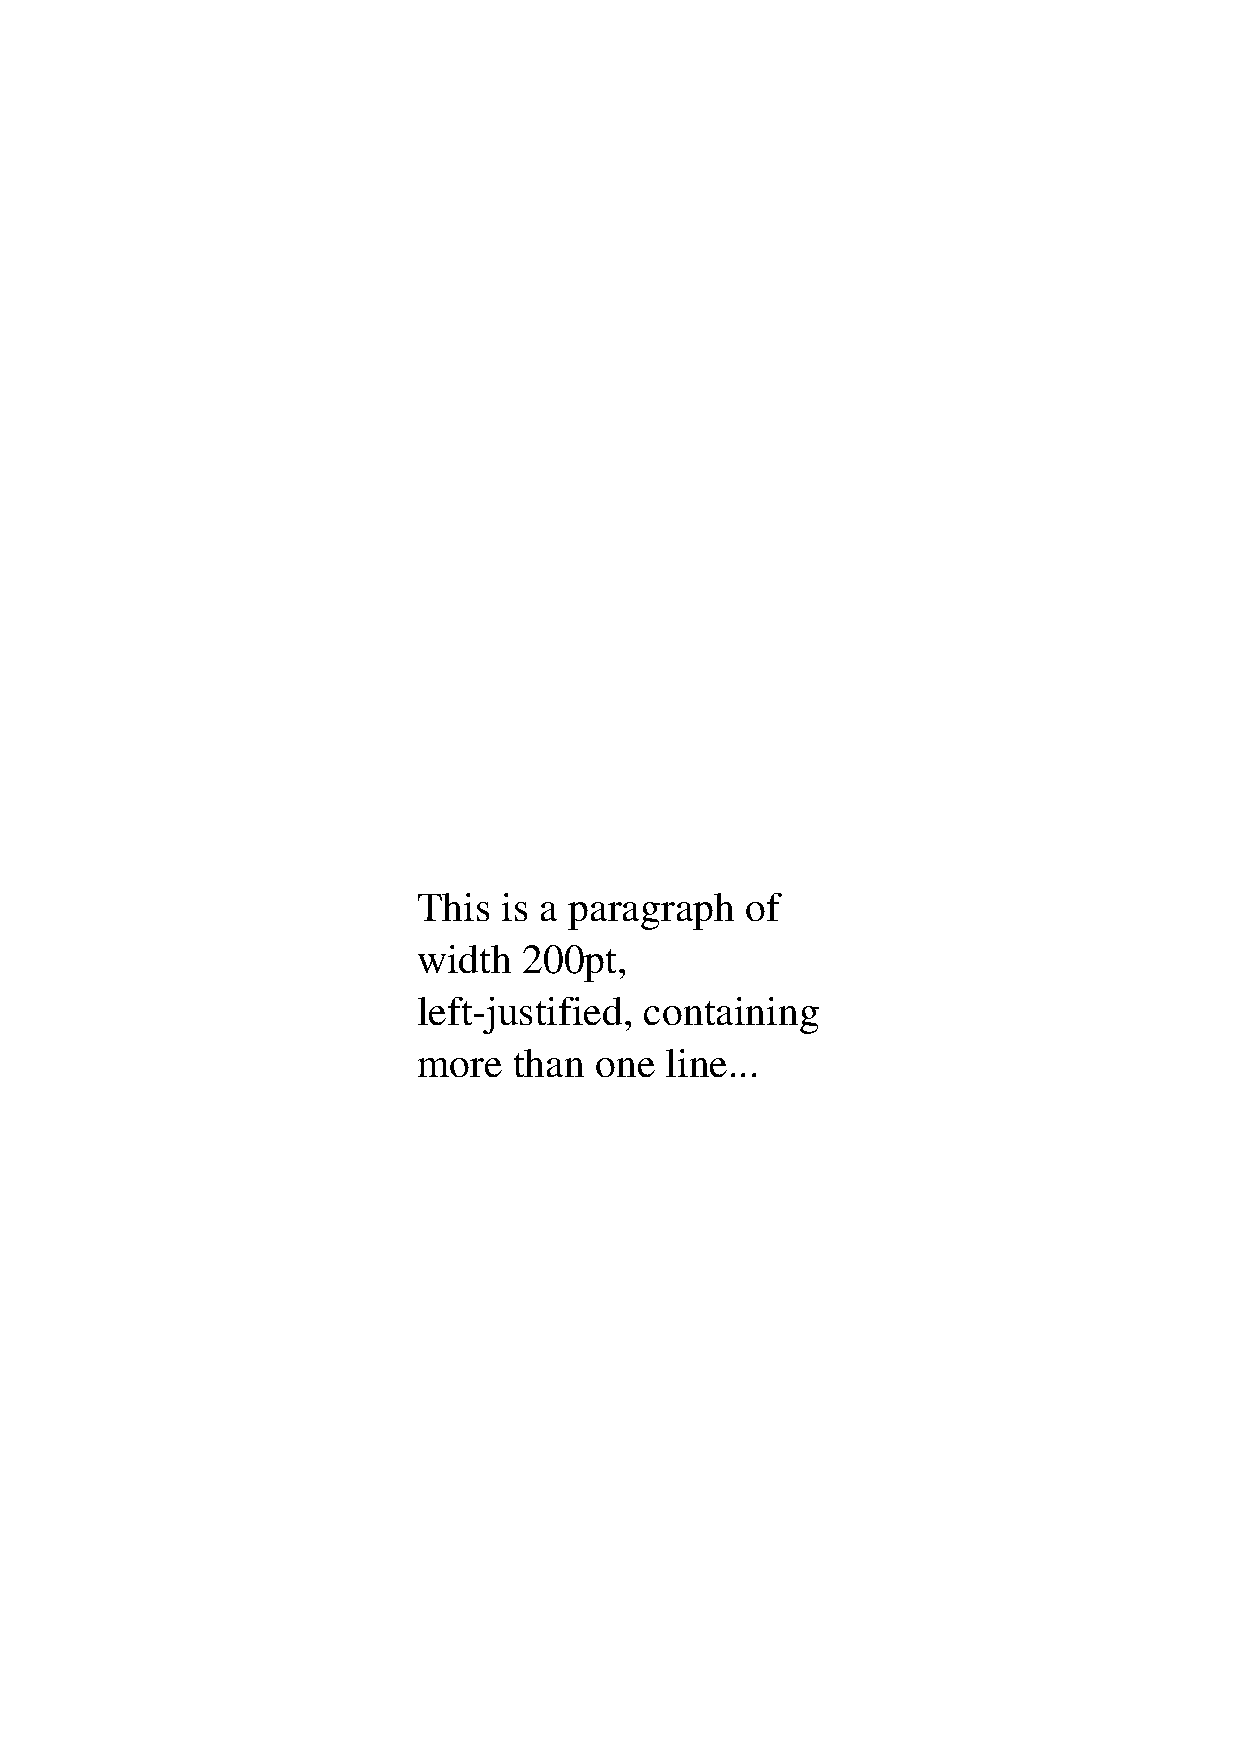
\includegraphics[natwidth=298,natheight=421,alt={A paragraph}]{manualimages/para.pdf}}
\else
\fbox{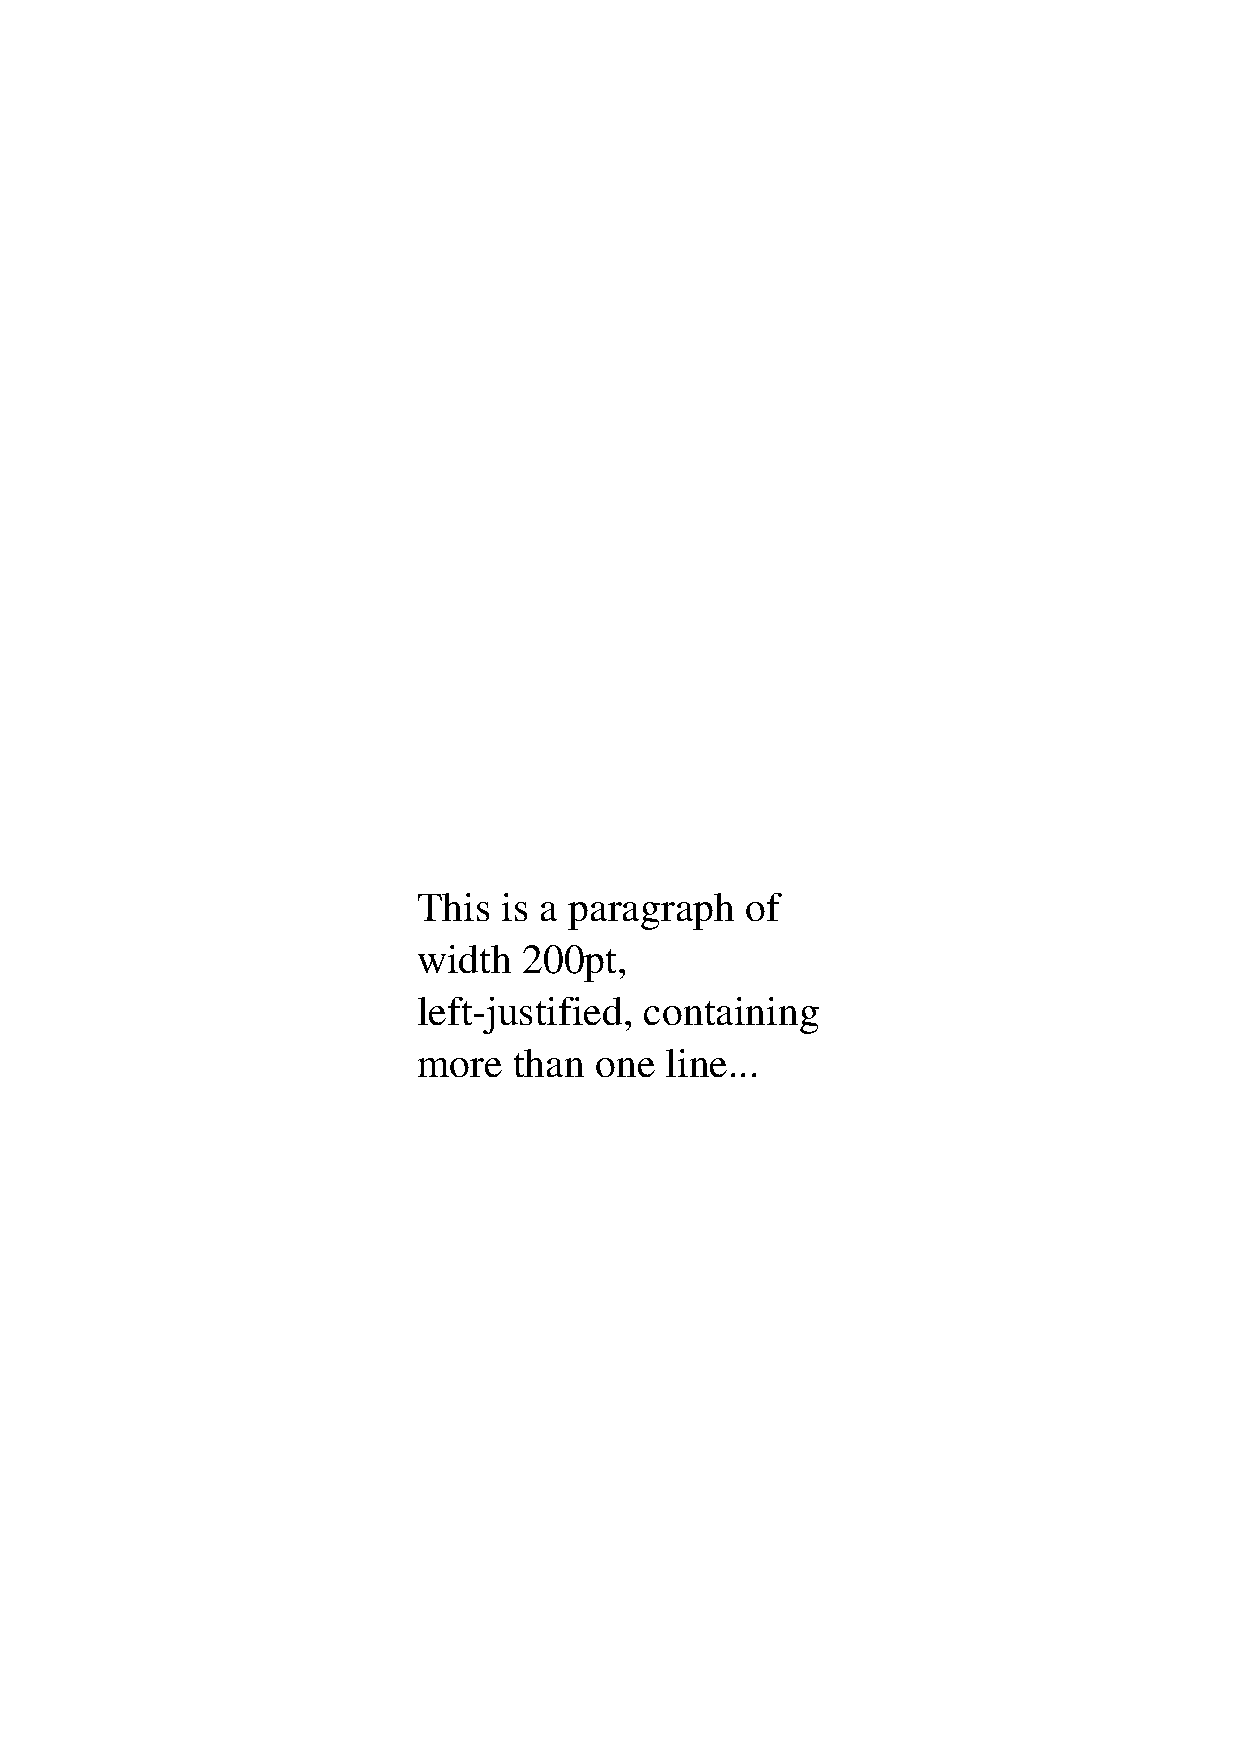
\includegraphics[width=0.3\textwidth,alt={A paragraph}]{manualimages/para.pdf}}
\fi
\bigskip

\noindent Multiple paragraphs with optional indenting may be laid out with \texttt{-paras}:

\begin{framed}
 \noindent\small\verb?cpdf -create-pdf AND -draw -mtrans "200 500" -bt -font-size 20 -leading 25?\\
 \noindent\small\verb?     -indent 20 -paras "L300=This is the first paragraph, which is spread ?\\
 \noindent\small\verb?     over multiple lines at this width...\nAnd here is the second, also ta?\\
 \noindent\small\verb?     king more than one line.\nHere is a little one." -et AND -decompress?\\
 \noindent\small\verb?     -o out.pdf?
\end{framed}

\noindent We specify the newlines with \texttt{\textbackslash n}, and the indentation with \texttt{-indent}. Here is the result.

\noindent

\bigskip
\ifdefined\HCode
\fbox{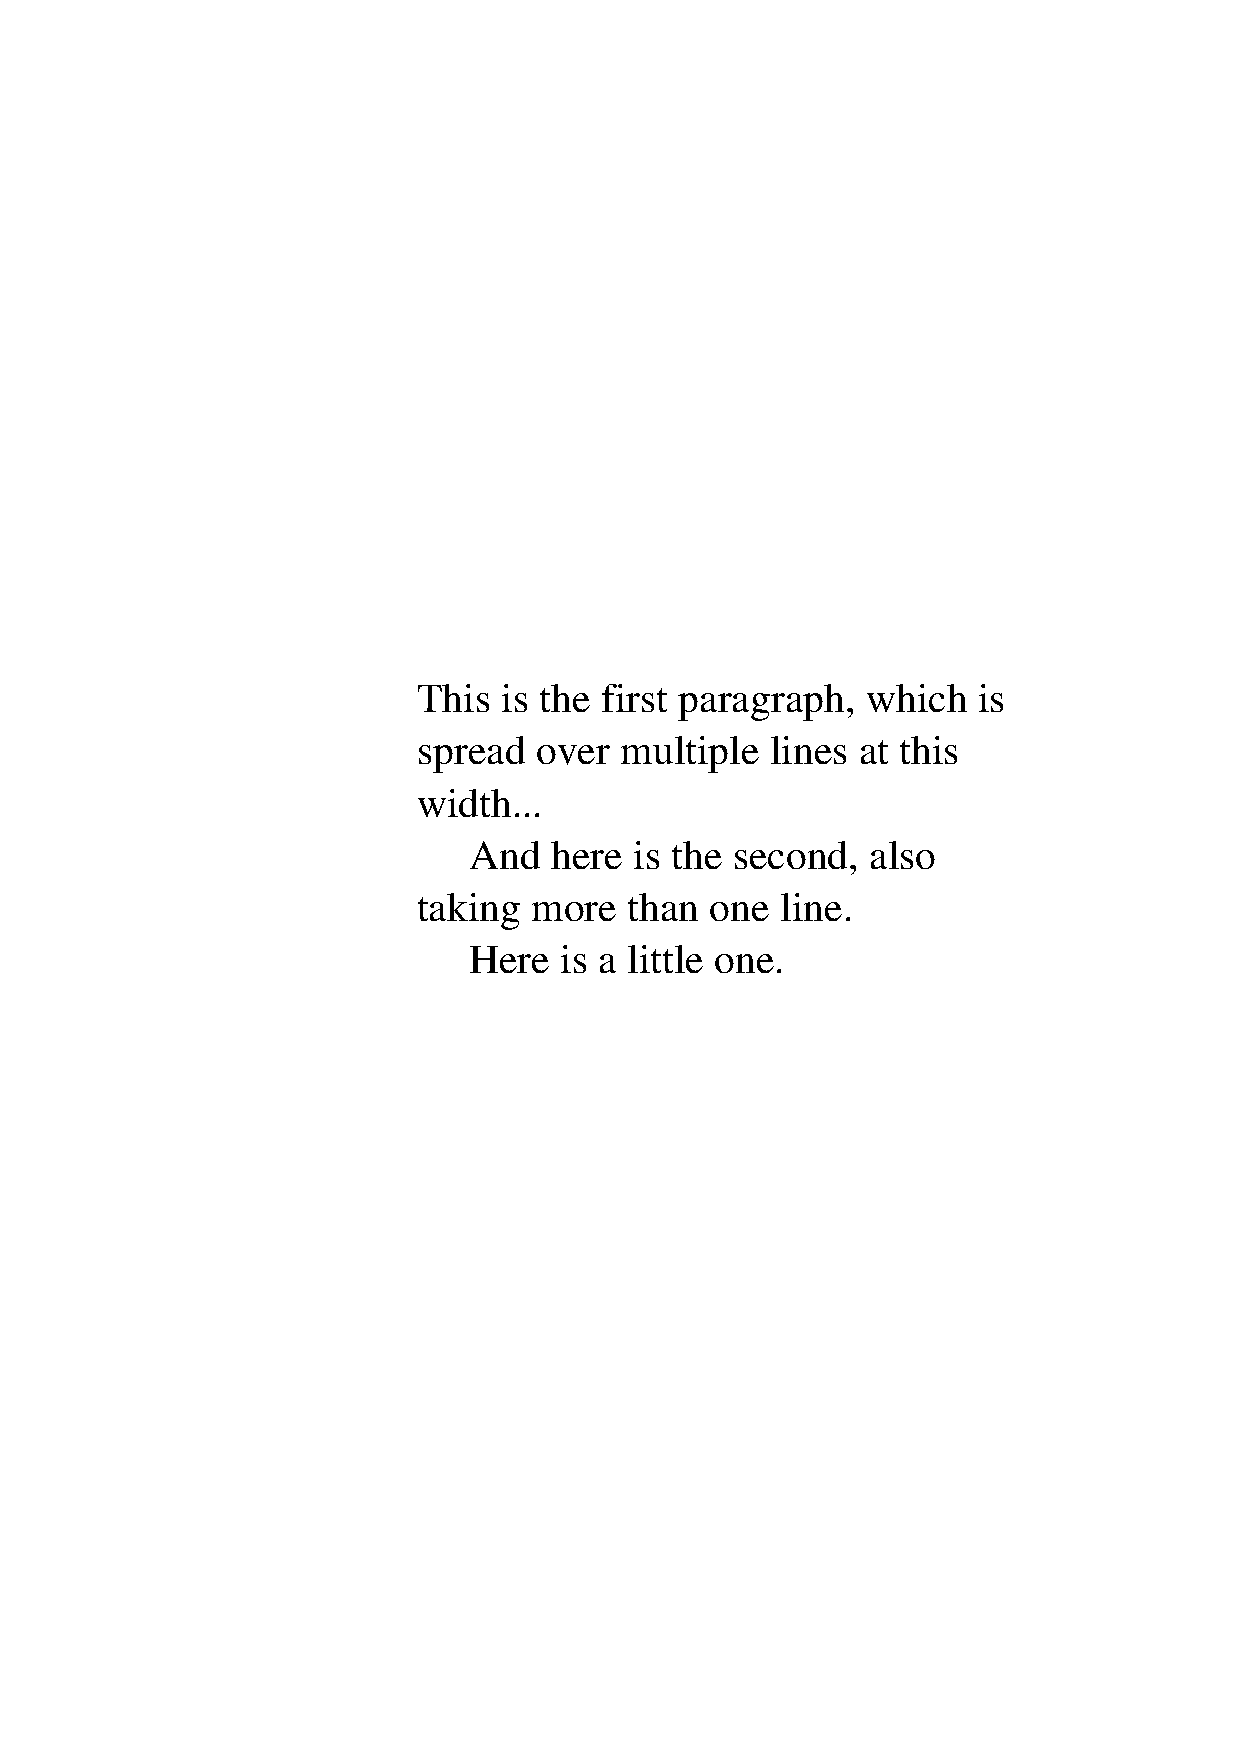
\includegraphics[natwidth=298,natheight=421,alt={Multiple paragraphs}]{manualimages/paras.pdf}}
\else
\fbox{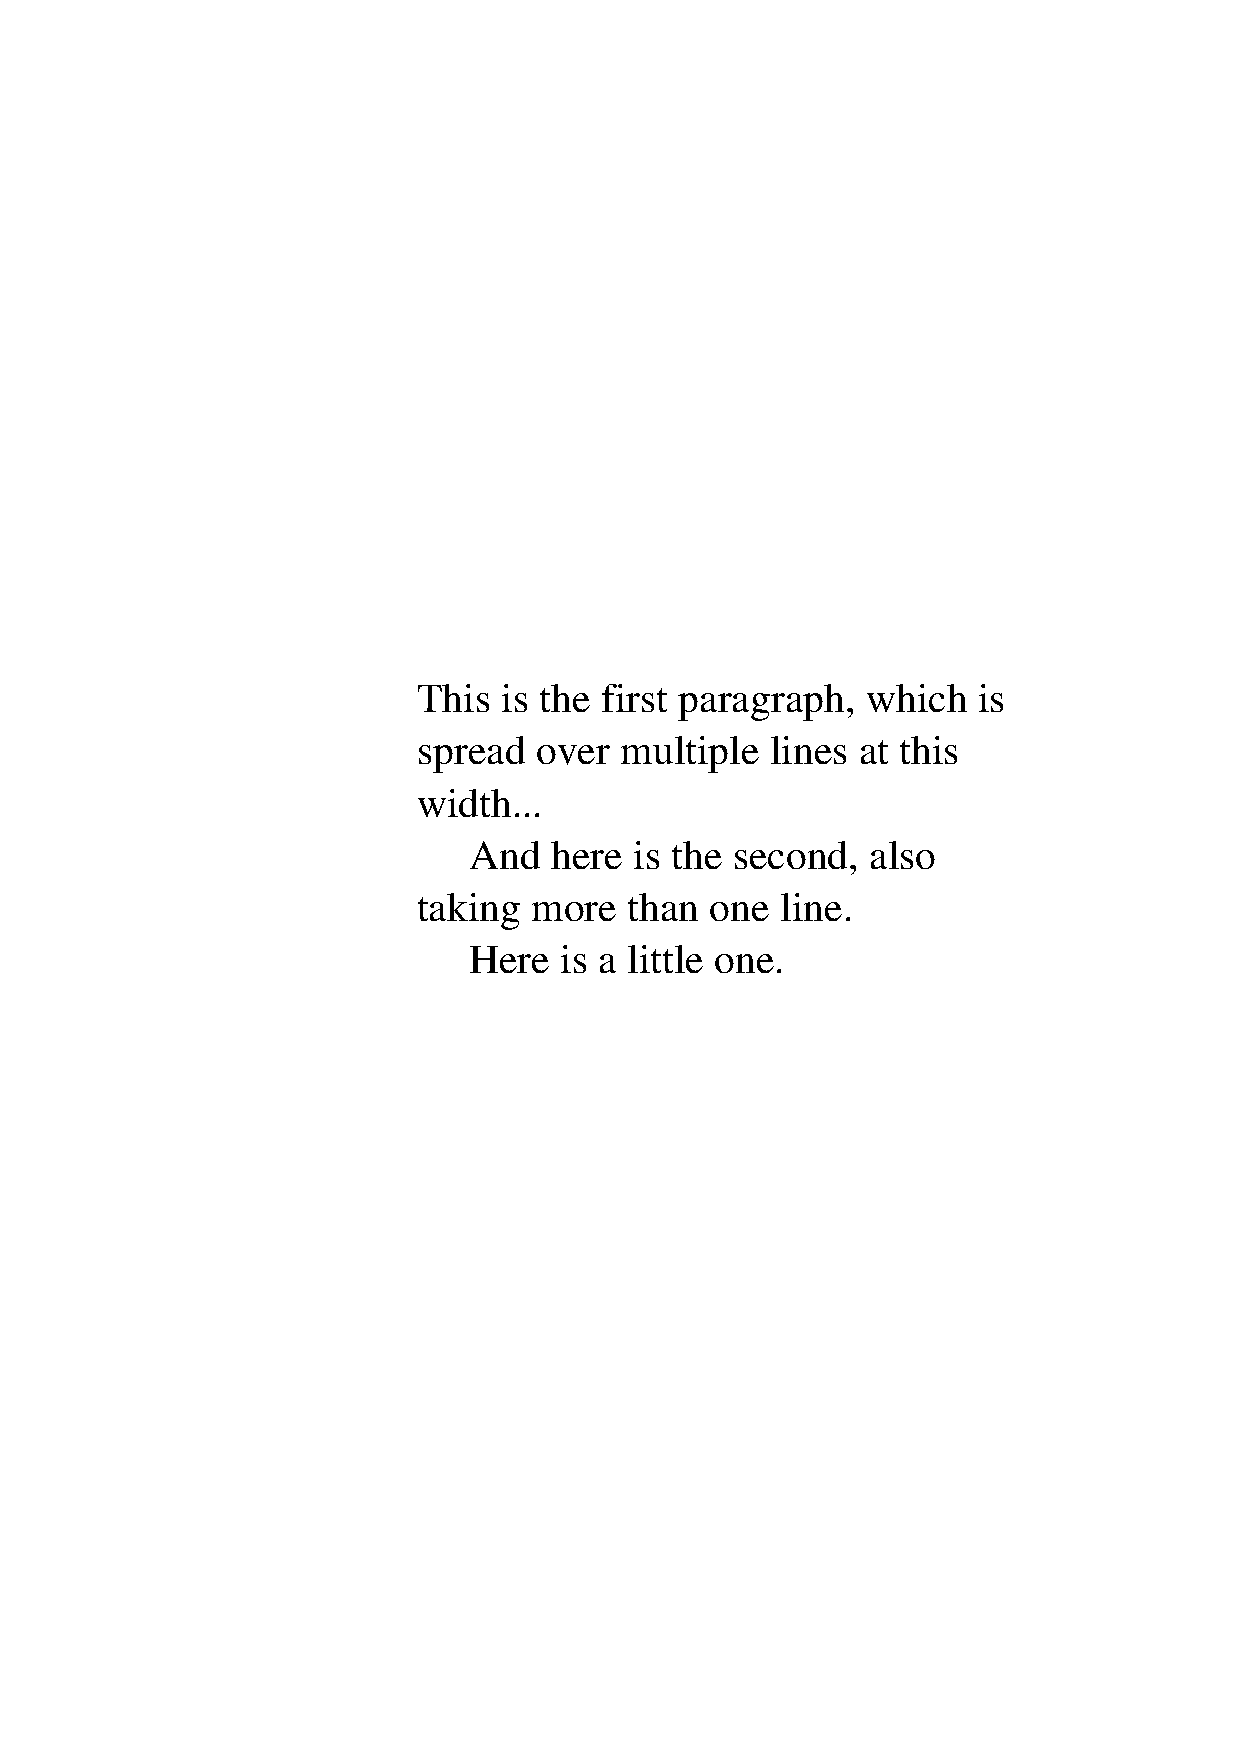
\includegraphics[width=0.3\textwidth,alt={Multiple paragraphs}]{manualimages/paras.pdf}}
\fi
\bigskip

\noindent Note that there is no automatic typesetting over multiple pages with \texttt{-paras}.

\section{The next page}

  {\small\begin{framed}
   \vspace{1.5mm}
   \noindent\verb!-newpage! Move to a fresh page
  \end{framed}}

If the drawing range is a single page, and the next page already exists, the drawing operation \texttt{-newpage} operation moves to the next page. Otherwise, it creates a fresh page of the same dimensions as the last page of the document, and sets the drawing range to just that page. For example:

\begin{framed}
 \noindent\small\verb?cpdf -create-pdf AND -draw -bt -text "Page 1" -et?\\
 \noindent\small\verb?     -newpage -bt -text "Page 2" -et?\\
 \noindent\small\verb?     -o out.pdf?
\end{framed}

\noindent This will create a two page PDF with "Page 1" written on page one and "Page 2" written on page two.

\section{Structure information}

A PDF may contain, in addition to its graphical content, a tree of information concerning the logical organization of the document into chapters, sections, paragraphs, figures and so on. When used with a standard set of pre-defined data types, this is known as Tagged PDF. Some PDF subformats, such as PDF/UA, mandate -- amongst other things -- the full tagging of the file.

When drawing on a fresh file, Cpdf can add such structure information. Partly this can happen automatically, partly it is for the user to add the tags. When drawing on an existing file, the new drawing is marked as an artifact.

To enable the generation of structure information, we add \texttt{-draw-struct-tree} to our command. NB It must precede \texttt{-draw} on the command line.

\begin{framed}
   \noindent\small\verb!cpdf -create-pdf AND!\\
   \noindent\small\verb!     -draw-struct-tree -draw -bt -text "Hello, World" -et -o out.pdf!
\end{framed}

\noindent Structure information in a PDF is in the form of a tree. We can now show the structure tree, and see that our paragraph on page one has been automatically tagged by Cpdf:

\begin{verbatim}
$cpdf -print-struct-tree out.pdf
StructTreeRoot
└── P (1)\end{verbatim}

\noindent To prevent such automatic tagging, relying only on manual tags, use \texttt{-no-auto-tags}. The effect may be reversed at any point with \texttt{-auto-tags}. Unless told otherwise, Cpdf auto-tags text added using \texttt{-text}, \texttt{-stext} and \texttt{-paras} with tag P, and images with tag Figure.

There are two types of tag we can add manually. One kind is used to tag individual pieces of content. We do this with a \texttt{-tag}/\texttt{-end-tag} pair. Note that nesting is not permitted here. For example, let us tag a heading:

\begin{framed}
   \noindent\small\verb!cpdf -create-pdf AND -draw-struct-tree -draw -mtrans "50 700" !\\
   \noindent\small\verb!     -font-size 40 -no-auto-tags -tag H1 -bt -text "This is the heading"!\\
   \noindent\small\verb!     -et -end-tag -auto-tags -mtrans "0 -100" -font-size 20 -leading 25!\\
   \noindent\small\verb!     -bt -paras "L200pt=This is the first paragraph, which spreads over!\\
   \noindent\small\verb!more than one line\nHere is the second, which also has multiple lines..."!\\
   \noindent\small\verb!     -et -o out.pdf!
\end{framed}

\noindent We turned off auto-tagging with \texttt{-no-auto-tag}, then used \texttt{-tag H1} and \texttt{-end-tag} to tag the heading. Then we turned auto-tagging back on with \texttt{-auto-tag}. Here is the result, visually:

\bigskip
\ifdefined\HCode
\fbox{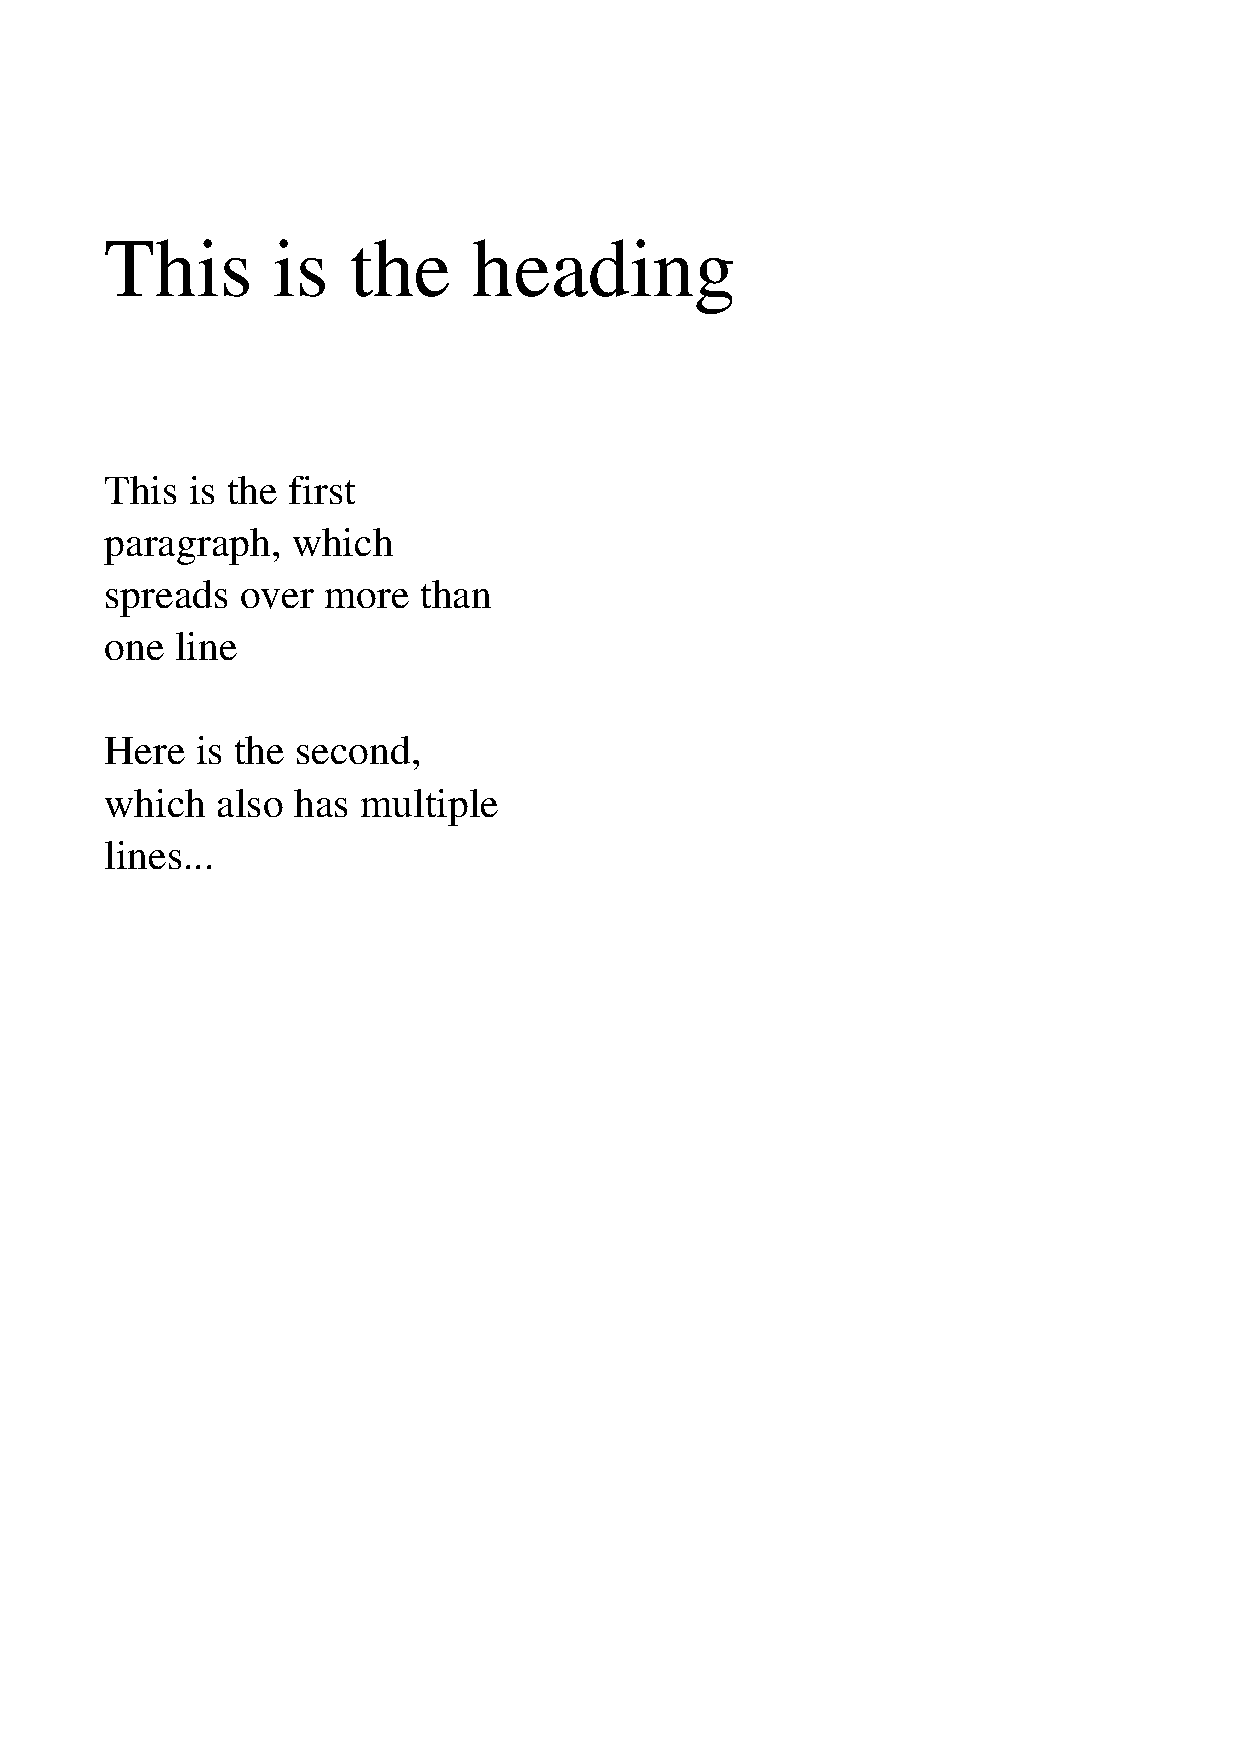
\includegraphics[natwidth=298,natheight=421,alt={Manual tagging}]{manualimages/h1.pdf}}
\else
\fbox{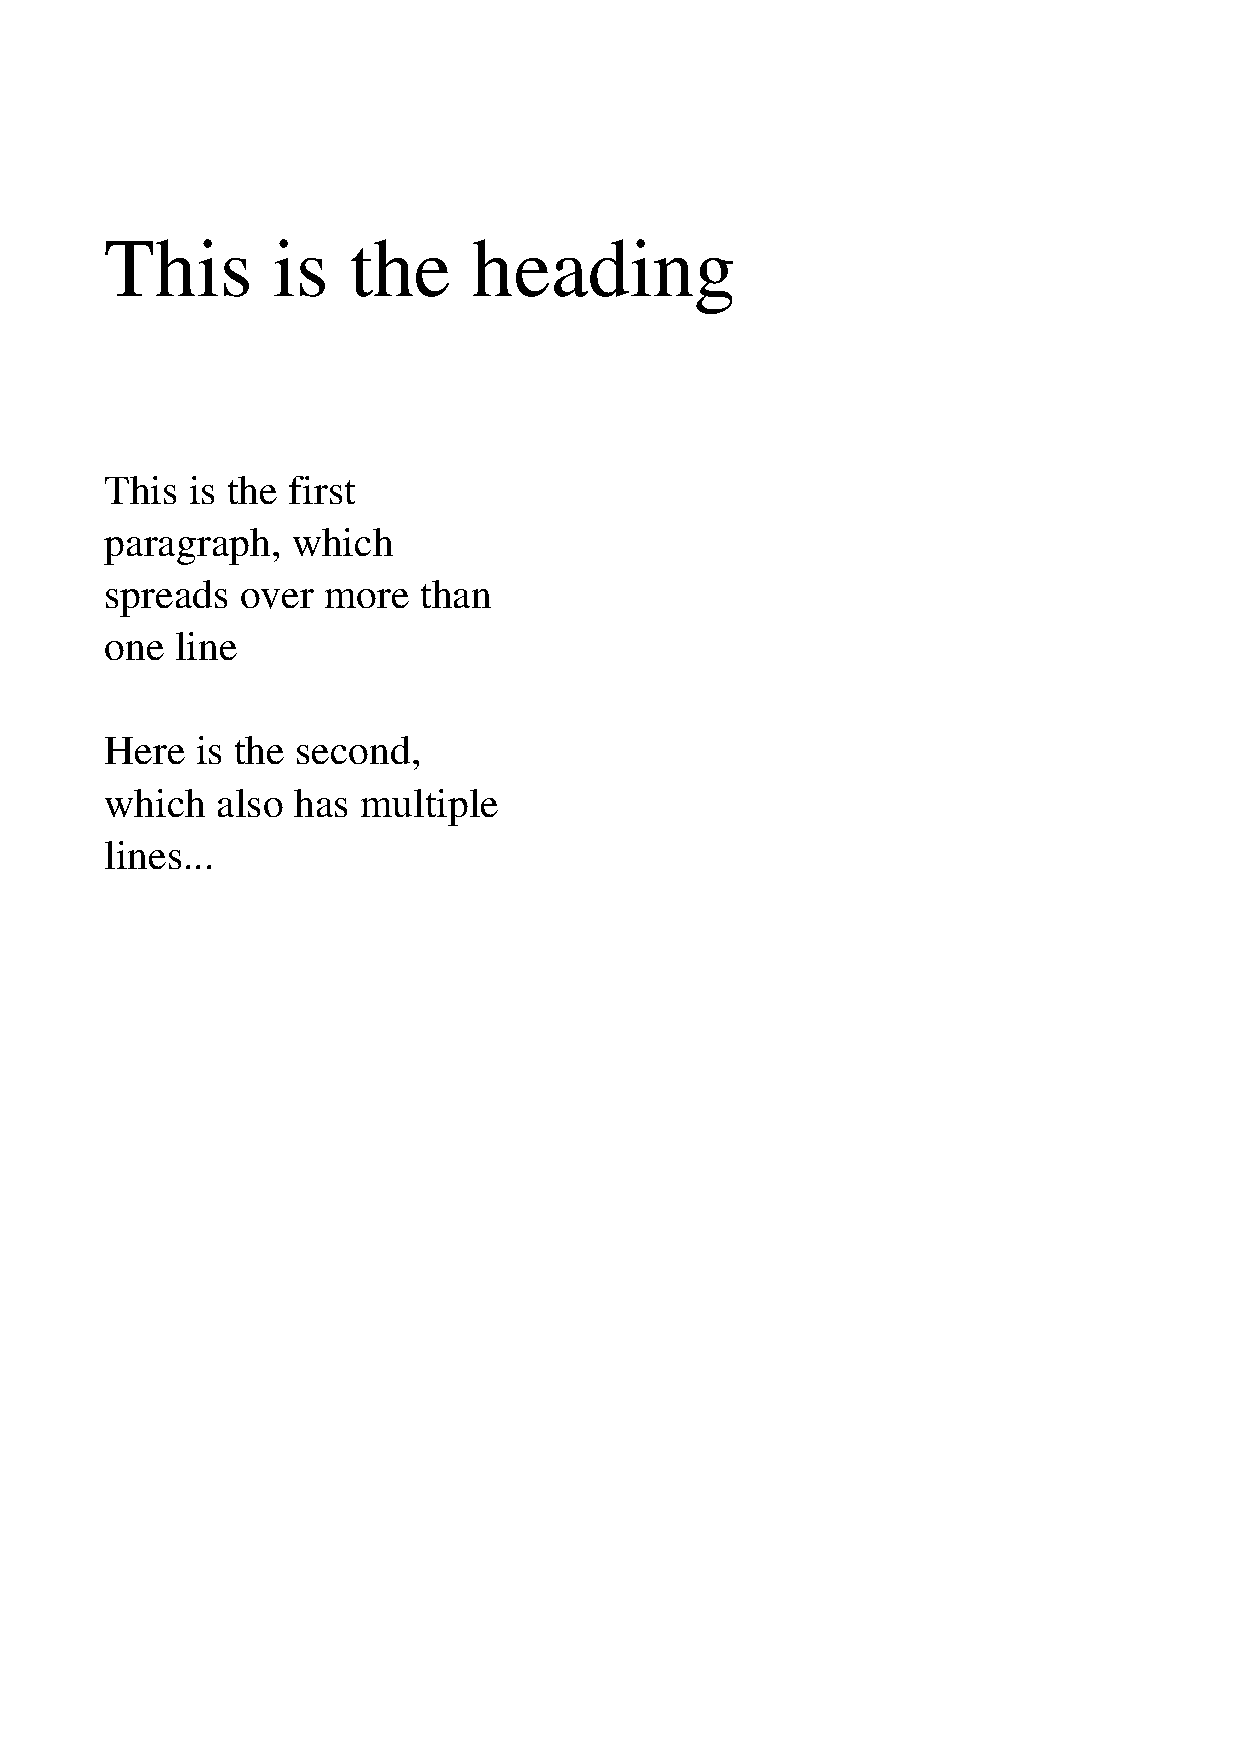
\includegraphics[width=0.3\textwidth,alt={Manual taggin}]{manualimages/h1.pdf}}
\fi
\bigskip

\noindent And here is the structure tree:

\begin{verbatim}
StructTreeRoot
├── H1 (1)
├── P (1)
└── P (1)
\end{verbatim}

\noindent Content tagging is flat - every part of the content of a page is part of only one \texttt{-tag}. The logical structure of a document, however, is a tree structure -- sections contain paragraphs, and so on. To build the logical structure tree, we add structure tags using \texttt{-stag} / \texttt{-end-stag} pairs which, of course, may be nested. For example, let's put our H1, and P sections in a Section structure tag:

\begin{framed}
   \noindent\small\verb!cpdf -create-pdf AND -draw-struct-tree -draw -mtrans "50 700" !\\
   \noindent\small\verb!     -font-size 40 -no-auto-tags -stag Section -tag H1 -bt!\\
   \noindent\small\verb!     -text "This is the heading" -et -end-tag -auto-tags -mtrans "0 -100" !\\
   \noindent\small\verb!     -font-size 20 -leading 25 -bt -paras "L200pt=This is the first parag!\\
   \noindent\small\verb!raph, which spreads over more than one line\nHere is the second, which al!\\
   \noindent\small\verb!so has multiple lines..." -et -end-stag -o out.pdf!
\end{framed}

\noindent Here is the structure tree:

\begin{verbatim}
StructTreeRoot
└──Section (1)
    ├── H1 (1)
    ├── P (1)
    └── P (1)
\end{verbatim}

\noindent Some PDF standards require that everything not marked as content (e.g paragraph, figure) etc. is marked as a an artifact. For example, a background image which is the same on every page, or a page border. This tells PDF processors that it is not logical content.

By default, Cpdf with \texttt{-draw-struct-tree} will mark anything not automatically or manually tagged as content as an artifact. Should you wish to disable this, you may use \texttt{-no-auto-artifacts}. Whether or not you use \texttt{-no-auto-artifacts}, you may use \texttt{-artifact} / \texttt{end-artifact} pairs to mark artifacts manually. For example:

\begin{framed}
   \noindent\small\verb!cpdf -create-pdf AND -draw-struct-tree -draw -no-auto-artifacts!\\
   \noindent\small\verb!     -artifact -mtrans "50 700" -end-artifact -bt -text "Hello" -et!\\
   \noindent\small\verb!     -o out.pdf!
\end{framed}

\noindent Here we manually tagged the \texttt{-mtrans} as being an artifact. The text section was automatically tagged as a paragraph, and so all content has been tagged or marked as an artifact.

Some tags require a namespace other than the default. You can set the namespace with \texttt{-namespace}, which affects all future tags until reset. Two namespace abbreviations are available: \texttt{PDF} for the default \texttt{http://iso.org/pdf/ssn} namespace and \texttt{PDF2} for the PDF 2.0 namespace \texttt{http://iso.org/pdf2/ssn}.

Extra information may be added to structure tree nodes with \texttt{-eltinfo} / \texttt{-end-eltinfo}. For example, to set the alternative description for an image, we might write (in JSON format, or prefixing with \texttt{PDF} in PDF format) \texttt{-eltinfo "Alt=PDF(A large horse)" -image A -end-eltinfo}. Multiple items may be set at once, for example Alt, ActualText, Lang etc. 

A role map, which maps non-standard structure types to standard ones, may be set with \texttt{-rolemap}. For example \texttt{-rolemap "/S1/H1/S2/H2"} would map the S1 structure type to the standard type H1 and so on.

To build a fresh PDF/UA or PDF/UA-2 file for use with \texttt{-draw} use \texttt{-create-pdf-ua-1} or \texttt{-create-pdf-ua-2} from chapter \ref{chap:19}.

\begin{cpdflib}
\clearpage
\section*{C Interface}
\begin{small}\tt
\lstinputlisting{docsplits/splits/c19}
\end{small}
\end{cpdflib}

\begin{pycpdflib}
\clearpage
\section*{Python Interface}
\begin{small}\tt
\lstinputlisting{docsplits/pysplits/c19}
\end{small}
\end{pycpdflib}

\begin{dotnetcpdflib}
\clearpage
\section*{.NET Interface}
\begin{small}\tt
\lstinputlisting{dotnetsplits/c19}
\end{small}
\end{dotnetcpdflib}

\begin{jcpdflib}
\clearpage
\section*{Java Interface}
\begin{small}\tt
\lstinputlisting{javasplits/c19}
\end{small}
\end{jcpdflib}

\begin{jscpdflib}
\clearpage
\section*{JavaScript Interface}
\begin{small}\tt
\lstinputlisting{docsplits/javascriptsplits/c19}
\end{small}
\end{jscpdflib}

\clearpage\pagestyle{empty}
\chapter{Accessible PDFs with PDF/UA}\label{chap:19}\pagestyle{fancy}\index{PDF/UA}\index{accessibility}

  {\small\begin{framed}
  \noindent\verb!cpdf -print-struct-tree in.pdf!

  \vspace{1.5mm}
  \noindent\verb!cpdf -extract-struct-tree in.pdf -o out.json!

  \vspace{1.5mm}
  \noindent\verb!cpdf -replace-struct-tree in.json in.pdf -o out.pdf!

  \vspace{1.5mm}
  \noindent\verb!cpdf -remove-struct-tree in.pdf -o out.pdf!

  \vspace{1.5mm}
  \noindent\verb!cpdf -mark-as-artifact in.pdf -o out.pdf!

  \vspace{1.5mm}
  \noindent\verb!cpdf -verify "PDF/UA-1(matterhorn)" [-json] in.pdf!

  \vspace{1.5mm}
  \noindent\verb!cpdf -verify "PDF/UA-1(matterhorn)" -verify-single <test> [-json] in.pdf!

  \vspace{1.5mm}
  \noindent\verb!cpdf -mark-as ["PDF/UA-1" | "PDF/UA-2"] in.pdf -o out.pdf!

  \vspace{1.5mm}
  \noindent\verb!cpdf -remove-mark ["PDF/UA-1" | "PDF/UA-2"] in.pdf -o out.pdf!

  \vspace{1.5mm}
  \noindent\verb!cpdf -create-pdf-ua-<1|2> <title> [-create-pdf-pages <n>]!\\
  \noindent\verb!      [-create-pdf-papersize <paper size>] -o out.pdf!

  \end{framed}}

PDF/UA (Universal Accessibility) is a PDF subformat whose rules consist of a set of machine-checkable and human-checkable-only requirements to make PDF documents accessible for all users - for example, those using screen readers. Cpdf has some basic facilities for manipulating the extra PDF constructs which are used in (amongst others) PDF/UA, and a basic verifier for many of the machine-checkable requirements.

\section{Structure trees}

In a PDF document, the optional Structure Tree is a parallel construct which describes the logical structure of a document (as opposed to the information for rendering the document on the screen or printing it out, which every PDF of course contains.)

We can print an abbreviated form of the structure tree to standard output:

  \begin{framed}
    \noindent\small\verb!cpdf -print-struct-tree in.pdf!
  \end{framed}

\noindent This might yield:

\smallgap

\begin{minipage}{\linewidth}
\begin{framed}
\begin{verbatim}
StructTreeRoot
└── Document
    ├── Sect
    │   ├── P (1)
    │   │   ├── Span (1)
    │   └── Figure (1)
    ├── Sect
    │   ├── H1 (2)
    │   └── TOC
    │       ├── TOCI
    │       │   └── P
    │       │       └── Link (2)
    .       .
    .       .
    .       .
\end{verbatim}
\end{framed}
\end{minipage}

\smallgap 
\noindent The numbers in parentheses are the page numbers for structure elements, where present. We can extract the full structure tree to JSON for inspection or manupulation:

  \begin{framed}
    \noindent\small\verb!cpdf -extract-struct-tree in.pdf -o out.json!
  \end{framed}

\noindent Here is a typical fragment:

{\small\begin{verbatim}
[
  [ 0, { "/CPDFJSONformatversion": 1, "/CPDFJSONpageobjnumbers": [ 52 ] } ],
  [
    102,
    {
      "/Type": { "N": "/StructElem" },
      "/S": { "N": "/TD" },
      "/P": 98,
      "/Pg": 52,
      "/K": { "I": 38 },
      "/T": { "U": "row #7, col #3" },
      "/A": {
        "/O": { "N": "/Layout" },
        "/Height": { "F": 18.28 },
        "/Width": { "F": 73.07689999999999 }
      }
    }
  ],
  [
    15,
    {
      "/Type": { "N": "/StructElem" },
      "/S": { "N": "/TD" },
      "/P": 59,
      "/Pg": 52,
      "/K": { "I": 20 },
      "/T": { "U": "row #3, col #5" },
      "/A": {
        "/O": { "N": "/Layout" },
        "/Height": { "F": 18.28 },
        "/Width": { "F": 73.07689999999999 }
      }
    }
  ],
...
\end{verbatim}}

\noindent This JSON file contains the structure tree objects from the file, using the format described in chapter \ref{chap:15}. There is a special entry in object \texttt{0} which gives the key to the page object numbers. In this example, there is one page with object number \texttt{52}.

This JSON file can be edited, for example to change text strings, and reapplied to the same file from which it was extracted:

  \begin{framed}
    \noindent\small\verb!cpdf -replace-struct-tree out.json in.pdf -o out.pdf!
  \end{framed}

\noindent If extra objects are required, they should be introduced with negative object numbers: Cpdf will renumber them on import so as not to clash with any existing numbers.

To remove a structure tree from a PDF, we can use \texttt{-remove-struct-tree}:

  \begin{framed}
    \noindent\small\verb!cpdf -remove-struct-tree in.pdf -o out.pdf!
  \end{framed}

\noindent This removes the structure tree and all references to it, including from inside page content. In addition we can, afterward, use \texttt{-mark-as-artifact}:

  \begin{framed}
    \noindent\small\verb!cpdf -mark-as-artifact in.pdf -o out.pdf!
  \end{framed}

\noindent This marks all content in the file as being an artifact.

\section{Verifying conformance to PDF/UA}

Cpdf contains a new, experimental verifier for PDF/UA via most of the machine-checkable subset of the Matterhorn Protocol, a list of checks based on the PDF/UA-1 specification. For example, we can run:

  \begin{framed}
    \noindent\small\verb!cpdf -verify "PDF/UA-1(matterhorn)" in.pdf!
  \end{framed}

\noindent We see:

{\small\begin{verbatim}
06-001 UA1:7.1-8 Document does not contain an XMP metadata stream 
07-001 UA1:7.1-9 ViewerPreferences dictionary of the Catalog dictionary does
not contain a DisplayDocTitle entry 
11-006 UA1:7.2-3 Natural language for document metadata cannot be determined.
("No top-level /Lang")
28-004 UA1:7.18.1-4 An annotation, other than of subtype Widget, does not
have a Contents entry and does not have an alternative description (in the
form of an Alt entry in the enclosing structure element). 
28-008 UA1:7.18.3-1 A page containing an annotation does not contain a Tabs
entry 
28-011 UA1:7.18.5-1 A link annotation is not nested within a <Link> tag. 
28-012 UA1:7.18.5-2 A link annotation does not include an alternate
description in its Contents entry. 
\end{verbatim}}

\noindent The first column here is the Matterhorn Protocol checkpoint, the second the reference in the PDF/UA-1 standard docunment, the third the textual description from the Matterhorn Protocol, and an optional fourth (in parentheses) any extra information available.

The same information is available in JSON format by adding \texttt{-json} to the command line:

{\small\begin{verbatim}
[
  {
    "name": "06-001",
    "section": "UA1:7.1-8",
    "error": "Document does not contain an XMP metadata stream",
    "extra": null
  },
  {
    "name": "07-001",
    "section": "UA1:7.1-9",
    "error": "ViewerPreferences dictionary of the Catalog dictionary does not
contain a DisplayDocTitle entry",
    "extra": null
  },
  {
    "name": "11-006",
    "section": "UA1:7.2-3",
    "error": "Natural language for document metadata cannot be determined.",
    "extra": "No top-level /Lang"
  },
  {
    "name": "28-004",
    "section": "UA1:7.18.1-4",
    "error": "An annotation, other than of subtype Widget, does not have a
Contents entry and does not have an alternative description (in the form of
an Alt entry in the enclosing structure element).",
    "extra": null
  },
  {
    "name": "28-008",
    "section": "UA1:7.18.3-1",
    "error": "A page containing an annotation does not contain a Tabs entry",
    "extra": null
  },
  {
    "name": "28-011",
    "section": "UA1:7.18.5-1",
    "error": "A link annotation is not nested within a <Link> tag.",
    "extra": null
  },
  {
    "name": "28-012",
    "section": "UA1:7.18.5-2",
    "error": "A link annotation does not include an alternate description in
its Contents entry.",
    "extra": null
  }\end{verbatim}}

\noindent If verifying many files for a single fault, we may choose which test to run by adding\linebreak \texttt{-verify-single <testname>} to the command line. For example:


  \begin{framed}
    \noindent\small\verb!cpdf -verify "PDF/UA-1(matterhorn)" -verify-single "28-012" in.pdf!
  \end{framed}

\noindent Presently, Matterhorn tests 31-001--016,018,030 are unimplemented. Matterhorn tests 31-027,10-001,11-001--005 are partially implemented. All others are implemented.

\section{PDF/UA compliance markers}

Once we are sure a file complies to PDF/UA, in terms of both machine and human checks, we can mark it as such:

  \begin{framed}
    \noindent\small\verb!cpdf -mark-as "PDF/UA-1" in.pdf -o out.pdf!
  \end{framed}

\noindent Or, for the more recent PDF/UA-2 standard:

  \begin{framed}
    \noindent\small\verb!cpdf -mark-as "PDF/UA-2" in.pdf -o out.pdf!
  \end{framed}

\noindent To remove such a marker we can use, for example:

  \begin{framed}
    \noindent\small\verb!cpdf -remove-mark "PDF/UA-1" in.pdf -o out.pdf!
  \end{framed}

\section{Merging and splitting PDF/UA files}

\noindent The \texttt{-process-struct-trees} option should always be used in conjunction with any splitting or merging command to preserve PDF/UA compliance. Sometimes \texttt{-subformat} may be required too. Details are given in chapter \ref{chap:2}.

\section{Creating new PDF/UA files}

To create a new PDF/UA-1 file, with A4 portrait paper, one page, and the title \texttt{"My Book"}, we may write:

  \begin{framed}
    \noindent\small\verb!cpdf -create-pdf-ua-1 "My Book" -o out.pdf!
  \end{framed}

\noindent A title is needed for every PDF/UA document (even a blank one) for it to meet the standard. For \texttt{PDF/UA-2}, use \texttt{-create-pdf-ua-2} instead. To make it valid, you must also draw a top-level PDF/UA-2 Document tag as described below i.e:

\begin{framed}
  \noindent\small\verb!cpdf -create-pdf-ua-2 "My Book" AND -draw -draw-struct-tree!\\
  \noindent\small\verb!     -namespace PDF2 -stag Document -end-stag -o out.pdf!
\end{framed}

\section{Drawing PDF/UA files}

Cpdf can add PDF/UA structure data when drawing on new PDF/UA files. For example the following produces a valid PDF/UA-1 file with structure information:

\begin{framed}
   \noindent\small\verb!cpdf -create-pdf-ua-1 "Hello" AND!\\
   \noindent\small\verb!     -embed-std14 /path/to/fonts -draw-struct-tree!\\
   \noindent\small\verb!     -draw -bt -text "Hello, World" -et -o out.pdf!
\end{framed}

\noindent Note we had to specify embedded fonts to make this a valid PDF/UA-1 file. To make a valid PDF/UA-2 file we must also add a top-level Document structure tag with the appropriate namespace. Here is the PDF/UA-2 version of our file:

\begin{framed}
   \noindent\small\verb!cpdf -create-pdf-ua-2 "Hello" AND !\\
   \noindent\small\verb!     -embed-std14 /path/to/fonts -draw-struct-tree!\\
   \noindent\small\verb!     -draw -namespace PDF2 -stag Document -namespace PDF!\\
   \noindent\small\verb!     -bt -text "Hello, World" -et -end-stag -o out.pdf!
\end{framed}

\noindent See chapter \ref{chap:18} for more details about adding structure information when drawing.

%FIXME PDF/UA-2 as well?
\section{Remediation of PDF/UA verification errors}

Remediation of a file which claims to match PDF/UA but which does not (either failing human or mechanical tests) is a complex topic. In this section, we list possible remediations for a file which fails mechanical verification with Cpdf or another verification tool. Sometimes these will be clear and simple -- for example where some piece of document metadata is missing -- and sometimes they will be almost impossible. Of course, often the truth lies between those two extremes.  

When all else fails, it may be possible to modify the basic structures of the PDF manually. This may be done by extracting the PDF to JSON using \texttt{-output-json} from chapter \ref{chap:15}, modifying the file manually in a text editor or automatically with a JSON processing tool such as \texttt{jq} and converting back to a PDF with \texttt{-j}. If the remediation requires altering page content streams, the option \texttt{-output-json-parse-content-streams} may be used. 

\subsection{Remediation List}

The following table lists each mechanically-verifiable test from the Matterhorn protocol. For each, we give the number, description from the Matterhorn protocol, and the reference into the PDF/UA standard. Then we describe, if possible, how to use Cpdf to remediate the failure. Sometimes this is a definitive command, sometimes a last-ditch attempt to re-process the file (to embed missing fonts or correct font structures, for example) and sometimes simply a direction to try the manual remediation procedure described above.

\newcommand{\norem}{File does not meet Tagged PDF standard - only manual remediation possible (see description above this table).}
\newcommand{\noremua}{File does not meet PDF/UA tagging standard - only manual remediation possible (see description above this table).}
\newcommand{\manonly}{File does not meet PDF/UA standard - only manual remediation possible (see description above this table).}
\newcommand{\gsfonts}{It is possible that reprocessing the file with \texttt{gs} using \texttt{cpdf in.pdf -gs gs -gs-malformed-force -o out.pdf [-gs-quiet]} will correct the fonts.}
\newcommand{\remannot}{If annotations are not required, they may be removed with \texttt{cpdf -remove-annotations in.pdf -o out.pdf}.}
\newcommand{\delannot}{Alternatively, use \texttt{-output-annotations-json} and \texttt{-set-annotations-json} as described in Chapter \ref{chap:10} to remove one or more specific annotations.}
\newcommand{\edittree}{Alternatively, edit the tree manually using \texttt{-extract-struct-tree} and \texttt{-replace-struct-tree} from this chapter.}
\newcommand{\setlang}{Assuming the document is all in a single language, set the top-level language with, for example, \texttt{cpdf -set-language "en-US" in.pdf -o out.pdf}. If the document contains multiple languages, only manual remediation is possible.}

\bgroup
\def\arraystretch{1.5}
\noindent\begin{longtable}{lp{10cm}l}
  \textbf{\textsc{Number}} & \textbf{\textsc{Description}} & \textbf{\textsc{Reference}}\\\endhead
  \textbf{01-003} & \textbf{Content marked as Artifact is present inside tagged content.} & \textbf{UA1:7.1-1}\\
  \textbf{01-004} & \textbf{Tagged content is present inside content marked as Artifact.} & \textbf{UA1:7.1-1}\\
  \textbf{01-005} & \textbf{Content is neither marked as Artifact nor tagged as real content.} & \textbf{UA1:7-1-2}\\
\multicolumn{3}{p{\dimexpr\linewidth-4\tabcolsep\relax}}{\norem}\\
  \textbf{01-007} & \textbf{Suspects entry has a value of true.} & \textbf{UA1:7-1-11}\\
\multicolumn{3}{p{\dimexpr\linewidth-4\tabcolsep\relax}}{If you are sure the file conforms to tagged PDF conventions, use \texttt{cpdf -replace-obj /Root/MarkInfo/Suspects=false in.pdf -o out.pdf}.}\\

\textbf{02-001} & \textbf{One or more non-standard tag’s mapping does not terminate with a standard type.} & \textbf{UA1:7.1-3}\\

  \textbf{02-003} & \textbf{A circular mapping exists.} & \textbf{UA1:7.1-3}\\

  \textbf{02-004} & \textbf{One or more standard types are remapped.} & \textbf{UA1:7.1-4}\\
\multicolumn{3}{p{\dimexpr\linewidth-4\tabcolsep\relax}}{\noremua}\\

  \textbf{06-001} & \textbf{Document does not contain an XMP metadata stream} & \textbf{UA1:7.1-8}\\
\multicolumn{3}{p{\dimexpr\linewidth-4\tabcolsep\relax}}{Create XMP metadata from any existing old-style metadata in the file with \texttt{cpdf -create-metadata in.pdf -o out.pdf}. This may lead to further verification errors due to empty metadata entries.}\\

  \textbf{06-002} & \textbf{The XMP metadata stream in the Catalog dictionary does not include the PDF/UA identifier.} & \textbf{UA1:5}\\
\multicolumn{3}{p{\dimexpr\linewidth-4\tabcolsep\relax}}{Mark the file as PDF/UA using \texttt{cpdf -mark-as ["PDF/UA-1" | "PDF/UA-2"] in.pdf -o out.pdf}.}\\

  \textbf{06-003} & \textbf{XMP metadata stream does not contain dc:title} & \textbf{UA1:7.1-8}\\
\multicolumn{3}{p{\dimexpr\linewidth-4\tabcolsep\relax}}{Add a title using \texttt{cpdf -set-title "My title" -also-set-xmp in.pdf -o out.pdf}.}\\

  \textbf{07-001} & \textbf{ViewerPreferences dictionary of the Catalog dictionary does not contain a DisplayDocTitle entry} & \textbf{UA1:7.1-9}\\
\multicolumn{3}{p{\dimexpr\linewidth-4\tabcolsep\relax}}{Add the entry with \texttt{cpdf -display-doc-title true in.pdf -o out.pdf}.}\\

  \textbf{07-002} & \textbf{ViewerPreferences dictionary of the Catalog dictionary contains a DisplayDocTitle entry with a value of false} & \textbf{UA1:7.1-9}\\
\multicolumn{3}{p{\dimexpr\linewidth-4\tabcolsep\relax}}{Replace the entry with \texttt{cpdf -display-doc-title true in.pdf -o out.pdf}.}\\

  \textbf{09-004} & \textbf{A table-related structure element is used in a way that does not conform to the syntax defined in ISO 32000-1, Table 337.} & \textbf{UA1-7.2-1}\\

  \textbf{09-005} & \textbf{A list-related structure element is used in a way that does not conform to Table 336 in ISO 32000-1.} & \textbf{UA1-7.2-1}\\

  \textbf{09-006} & \textbf{A TOC-related structure element is used in a way that does not conform to Table 333 in ISO 32000-1.} & \textbf{UA1-7.2-1}\\

  \textbf{09-007} & \textbf{A Ruby-related structure element is used in a way that does not conform to Table 338 in ISO 32000-1.} & \textbf{UA1-7.2-1}\\

  \textbf{09-008} & \textbf{A Warichu-related structure element is used in a way that does not conform to Table 338 in ISO 32000-1.} & \textbf{UA1-7.2-1}\\
\multicolumn{3}{p{\dimexpr\linewidth-4\tabcolsep\relax}}{\noremua}\\

  \textbf{10-001} & \textbf{Character code cannot be mapped to Unicode.} & \textbf{UA1:7.2-2}\\
\multicolumn{3}{p{\dimexpr\linewidth-4\tabcolsep\relax}}{\gsfonts}\\

  \textbf{11-001} & \textbf{Natural language for text in page content cannot be determined.} & \textbf{UA1:7.2-3}\\

  \textbf{11-002} & \textbf{Natural language for text in Alt, ActualText and E attributes cannot be determined.} & \textbf{UA1:7.2-3}\\

  \textbf{11-003} & \textbf{Natural language in the Outline entries cannot be determined.} & UA1:7.2-3\\

  \textbf{11-004} & \textbf{Natural language in the Contents entry for annotations cannot be determined.} & \textbf{UA1:7.2-3}\\

  \textbf{11-005} & \textbf{Natural language in the TU entry for form fields cannot be determined.} & \textbf{UA1:7.2-3}\\

  \textbf{11-006} & \textbf{Natural language for document metadata cannot be determined.} & \textbf{UA1:7.2-3}\\
\multicolumn{3}{p{\dimexpr\linewidth-4\tabcolsep\relax}}{\setlang}\\

  \textbf{13-004} & \textbf{\textless Figure\textgreater\ tag alternative or replacement text missing.} & \textbf{UA1:7.3-3}\\

  \textbf{14-002} & \textbf{Does use numbered headings, but the first heading tag is not \textless H1\textgreater .} & \textbf{UA1:7.4.2-1}\\

  \textbf{14-003} & \textbf{Numbered heading levels in descending sequence are skipped (Example: \textless H3\textgreater\  follows directly after \textless H1\textgreater{}).} & \textbf{UA1:7.4-1}\\

  \textbf{14-006} & \textbf{A node contains more than one \textless H\textgreater\ tag.} & \textbf{UA1:7.4.4-1}\\

  \textbf{14-007} & \textbf{Document uses both \textless H\textgreater\ and \textless H\#\textgreater\ tags.} & \textbf{UA1:7.4.4-3}\\

  \textbf{15-003} & \textbf{In a table not organized with Headers attributes and IDs, a \textless TH\textgreater\ cell does not contain a Scope attribute.} & \textbf{UA1:7.5-2}\\

  \textbf{17-002} & \textbf{\textless Formula\textgreater\ tag is missing an Alt attribute.} & \textbf{UA1:7.7-1}\\
\multicolumn{3}{p{\dimexpr\linewidth-4\tabcolsep\relax}}{\manonly\ \edittree}\\

  \textbf{17-003} & \textbf{Unicode mapping requirements are not met.} & \textbf{UA1:7.7-2}\\
\multicolumn{3}{p{\dimexpr\linewidth-4\tabcolsep\relax}}{\gsfonts}\\

  \textbf{19-003} & \textbf{ID entry of the \textless Note\textgreater\ tag is not present.} & \textbf{UA1:7.9-2}\\

  \textbf{19-004} & \textbf{ID entry of the \textless Note\textgreater\ tag is non-unique.} & \textbf{UA1:7.9-2}\\

  \textbf{20-001} & \textbf{Name entry is missing or has an empty string as its value in an Optional Content Configuration Dictionary in the Configs entry in the OCProperties entry in the Catalog dictionary.} & \textbf{UA1:7.10-1}\\

  \textbf{20-002} & \textbf{Name entry is missing or has an empty string as its value in an Optional Content Configuration Dictionary that is the value of the D entry in the OCProperties entry in the Catalog dictionary.} & \textbf{UA1:7.10-1}\\
\multicolumn{3}{p{\dimexpr\linewidth-4\tabcolsep\relax}}{\manonly\ \edittree}\\

  \textbf{20-003} & \textbf{An AS entry appears in an Optional Content Configuration Dictionary.} & \textbf{UA1:7.10-2}\\
\multicolumn{3}{p{\dimexpr\linewidth-4\tabcolsep\relax}}{\manonly}\\

  \textbf{21-001} & \textbf{The file specification dictionary for an embedded file does not contain F and UF entries.} & \textbf{UA1:7.11-1}\\
\multicolumn{3}{p{\dimexpr\linewidth-4\tabcolsep\relax}}{\manonly\ \edittree}\\

  \textbf{25-001} & \textbf{File contains the dynamicRender element with value “required”.} & \textbf{UA1:7.15-1}\\
\multicolumn{3}{p{\dimexpr\linewidth-4\tabcolsep\relax}}{Not remediable, unless actually a wrong marker. This is an interactive PDF form which likely only works with Adobe Acrobat. If the marker is actually wrong, it may be edited manually inside the XML stream using the instructions above.}\\

  \textbf{26-001} & \textbf{The file is encrypted but does not contain a P entry in its encryption dictionary.} & \textbf{UA1:7.16-1}\\

  \textbf{26-002} & \textbf{The file is encrypted and does contain a P entry but the 10th bit position of the P entry is false.} & \textbf{UA1:7.16-1}\\
\multicolumn{3}{p{\dimexpr\linewidth-4\tabcolsep\relax}}{Re-encrypt the file with Cpdf as described in Chapter 4.}\\

  \textbf{28-002} & \textbf{An annotation, other than of subtype Widget, Link and PrinterMark, is not a direct child of an \textless Annot\textgreater\ structure element.} & \textbf{UA1:7.18.1-2}\\

  \textbf{28-004} & \textbf{An annotation, other than of subtype Widget, does not have a Contents entry and does not have an alternative description (in the form of an Alt entry in the enclosing structure element).} & \textbf{UA1:7.18.1-4}\\

  \textbf{28-005} & \textbf{A form field does not have a TU entry and does not have an alternative description (in the form of an Alt entry in the enclosing structure element).} & \textbf{UA1:7.18.1-4}\\
\multicolumn{3}{p{\dimexpr\linewidth-4\tabcolsep\relax}}{\manonly\ \edittree}\\

  \textbf{28-006} & \textbf{An annotation with subtype undefined in ISO 32000 does not meet 7.18.1.} & \textbf{UA1:7.18.2-1}\\

  \textbf{28-007} & \textbf{An annotation of subtype TrapNet exists.} & \textbf{UA1:7.18.2-2}\\

  \textbf{28-008} & \textbf{A page containing an annotation does not contain a Tabs entry} & \textbf{UA1:7.18.3-1}\\

  \textbf{28-009} & \textbf{A page containing an annotation has a Tabs entry with a value other than S.} & \textbf{UA1:7.18.3-1}\\
\multicolumn{3}{p{\dimexpr\linewidth-4\tabcolsep\relax}}{\remannot\ \delannot}\\

  \textbf{28-010} & \textbf{A widget annotation is not nested within a \textless Form\textgreater\ tag.} & \textbf{UA1:7.18.4-1}\\

  \textbf{28-011} & \textbf{A link annotation is not nested within a \textless Link\textgreater\ tag.} & \textbf{UA1:7.18.5-1}\\
\multicolumn{3}{p{\dimexpr\linewidth-4\tabcolsep\relax}}{\remannot\ \delannot\ \edittree}\\

  \textbf{28-012} & \textbf{A link annotation does not include an alternate description in its Contents entry.} & \textbf{UA1:7.18.5-2}\\

  \textbf{28-014} & \textbf{CT entry is missing from the media clip data dictionary.} &\\

  \textbf{28-015} & \textbf{Alt entry is missing from the media clip data dictionary.} & \textbf{UA1:7.18.6.2-1}\\

  \textbf{28-016} & \textbf{File attachment annotations do not conform to 7.11.} & \textbf{UA1:7.18.7-1}\\
\multicolumn{3}{p{\dimexpr\linewidth-4\tabcolsep\relax}}{\remannot\ \delannot}\\

  \textbf{28-017} & \textbf{A PrinterMark annotation is included in the logical structure.} & \textbf{UA1:7.18.8-1}\\
\multicolumn{3}{p{\dimexpr\linewidth-4\tabcolsep\relax}}{\remannot\ \delannot\ \edittree}\\

  \textbf{28-018} & \textbf{The appearance stream of a PrinterMark annotation is not marked as Artifact.} & \textbf{UA1:7.18.8-2}\\
\multicolumn{3}{p{\dimexpr\linewidth-4\tabcolsep\relax}}{\remannot\ \delannot}\\

  \textbf{30-001} & \textbf{A reference XObject is present.} & \textbf{UA1:7.2}\\
\multicolumn{3}{p{\dimexpr\linewidth-4\tabcolsep\relax}}{A reference XObject references a page in another file. May be cut out manually using the manual remediation instructions above.}\\

  \textbf{30-002} & \textbf{Form XObject contains MCIDs and is referenced more than once.} & \textbf{UA1:7.21.3.1-1}\\
\multicolumn{3}{p{\dimexpr\linewidth-4\tabcolsep\relax}}{Unlikely to be remediable: the only option is to manually remove them, but this would then result in a tag tree pointing to non-existent MCIDs, which would be another kind of invalidity. Any PDF producer creating Tagged PDF with MCIDs like this is simply broken.}\\

  \textbf{31-001} & \textbf{A Type 0 font dictionary with encoding other than Identity-H and Identity-V has values for Registry in both CIDSystemInfo dictionaries that are not identical.} & \textbf{UA1:7.21.3-1}\\

  \textbf{31-002} & \textbf{A Type 0 font dictionary with encoding other than Identity-H and Identity-V has values for Ordering in both CIDSystemInfo dictionaries that are not identical.} & \textbf{UA1:7.21.3.1-1}\\

  \textbf{31-003} & \textbf{A Type 0 font dictionary with encoding other than Identity-H and Identity-V has a value for Supplement in the CIDSystemInfo dictionary of the CID font that is less than the value for Supplement in the CIDSystemInfo dictionary of the CMap.} & \textbf{UA1:7.21.3.1-1}\\

  \textbf{31-004} & \textbf{A Type 2 CID font contains neither a stream nor the name Identity as the value of the CIDToGIDMap entry.} & \textbf{UA1:7.21.3.2-1}\\

  \textbf{31-005} & \textbf{A Type 2 CID font does not contain a CIDToGIDMap entry.} & \textbf{UA1:7.21.3.2-1}\\

  \textbf{31-006} & \textbf{A CMap is neither listed as described in ISO 32000- 1:2008, 9.7.5.2, Table 118 nor is it embedded.} & \textbf{UA1:7.21.3.3-1}\\

  \textbf{31-007} & \textbf{The WMode entry in a CMap dictionary is not identical to the WMode value in the CMap stream.} & \textbf{UA1:7.21.3.3-1}\\

  \textbf{31-008} & \textbf{A CMap references another CMap which is not listed in ISO 32000-1:2008, 9.7.5.2, Table 118.} & \textbf{UA1:7.21.3.3-2}\\

  \textbf{31-009} & \textbf{For a font used by text intended to be rendered the font program is not embedded.} & \textbf{UA1:7.21.4.1-1}\\

  \textbf{31-011} & \textbf{For a font used by text the font program is embedded but it does not contain glyphs for all of the glyphs referenced by the text used for rendering.} & \textbf{UA1:7.21.4.1-3}\\

  \textbf{31-012} & \textbf{The FontDescriptor dictionary of an embedded Type 1 font contains a CharSet string, but at least one of the glyphs present in the font program is not listed in the CharSet string.} & \textbf{UA1:7.21.4.2-1}\\

  \textbf{31-013} & \textbf{The FontDescriptor dictionary of an embedded Type 1 font contains a CharSet string, but at least one of the glyphs listed in the CharSet string is not present in the font program.} & \textbf{UA1:7.21.4.2-2}\\

  \textbf{31-014} & \textbf{The FontDescriptor dictionary of an embedded CID font contains a CIDSet string, but at least one of the glyphs present in the font program is not listed in the CIDSet string.} & \textbf{UA1:7.21.4.2-3}\\

  \textbf{31-015} & \textbf{The FontDescriptor dictionary of an embedded CID font contains a CIDSet string, but at least one of the glyphs listed in the CIDSet string is not present in the font program.} & \textbf{UA1:7.21.4.2-4}\\

  \textbf{31-016} & \textbf{For one or more glyphs, the glyph width information in the font dictionary and in the embedded font program differ by more than 1/1000 unit.} & \textbf{UA1:7.21.5-1}\\

  \textbf{31-017} & \textbf{A non-symbolic TrueType font is used for rendering, but none of the cmap entries in the embedded font program is a non-symbolic cmap.} & \textbf{UA1:7.21.6-1}\\

  \textbf{31-018} & \textbf{A non-symbolic TrueType font is used for rendering, but for at least one glyph to be rendered the glyph cannot be looked up by any of the non-symbolic cmap entries in the embedded font program.} & \textbf{UA1:7.21.6-2}\\

  \textbf{31-019} & \textbf{The font dictionary for a non-symbolic TrueType font does not contain an Encoding entry.} & \textbf{UA1:7.21.6-3}\\

  \textbf{31-020} & \textbf{The font dictionary for a non-symbolic TrueType font contains an Encoding dictionary which does not contain a BaseEncoding entry.} & \textbf{UA1:7.21.6-4}\\

  \textbf{31-021} & \textbf{The value for either the Encoding entry or the BaseEncoding entry in the Encoding dictionary in a non-symbolic TrueType font dictionary is neither MacRomanEncoding nor WinAnsiEncoding.} & \textbf{UA1:7.21.6-5}\\

  \textbf{31-022} & \textbf{The Differences array in the Encoding entry in a non-symbolic TrueType font dictionary contains one or more glyph names which are not listed in the Adobe Glyph List.} & \textbf{UA1:7.21.6-6}\\

  \textbf{31-023} & \textbf{The Differences array is present in the Encoding entry in a non-symbolic TrueType font dictionary but the embedded font program does not contain a (3,1) Microsoft Unicode cmap.} & \textbf{UA1:7.21.6-7}\\

  \textbf{31-024} & \textbf{The Encoding entry is present in the font dictionary for a symbolic TrueType font.} & \textbf{UA1:7.21.6-8}\\

  \textbf{31-025} & \textbf{The embedded font program for a symbolic TrueType font contains no cmap.} & \textbf{UA1:7.21.6-9}\\

  \textbf{31-026} & \textbf{The embedded font program for a symbolic TrueType font contains more than one cmap, but none of the cmap entries is a (3,0) Microsoft Symbol cmap.} & \textbf{UA1:7.21.6-10}\\

  \textbf{31-027} & \textbf{A font dictionary does not contain the ToUnicode entry and none of the following is true: the font uses MacRomanEncoding, MacExpertEncoding or WinAnsiEncoding; the font is a Type 1 or Type 3 font and the glyph names of the glyphs referenced are all contained in the Adobe Glyph List or the set of named characters in the Symbol font, as defined in ISO 32000-1:2008, Annex D; the font is a Type 0 font, and its descendant CIDFont uses Adobe-GB1, Adobe-CNS1, Adobe-Japan1 or Adobe-Korea1 character collections; the font is a non-symbolic TrueType font.} & \textbf{UA1:7.21.7-1}\\

  \textbf{31-028} & \textbf{One or more Unicode values specified in the ToUnicode CMap are zero (0).} & \textbf{UA1:7.21.7-2}\\

  \textbf{31-029} & \textbf{One or more Unicode values specified in the ToUnicode CMap are equal to either U+FEFF or U+FFFE.} & \textbf{UA1:7.21.7-3}\\

  \textbf{31-030} & \textbf{One or more characters used in text showing operators reference the .notdef glyph.} & \textbf{UA1:7.21.8-1}\\
\multicolumn{3}{p{\dimexpr\linewidth-4\tabcolsep\relax}}{\gsfonts}\\

\end{longtable}
\egroup

\clearpage\pagestyle{empty}
%We wanted to call this "Chapter M", but the following commands messed up the PDF bookmarks, so this chapter will simply have to float for now, until we can return to this problem.
%\setcounter{chapter}{12}
%\renewcommand{\thechapter}{\Alph{chapter}}%
\chapter{Miscellaneous}\label{chap:misc}\pagestyle{fancy}
  {\small\begin{framed}
  \noindent\verb!cpdf -draft [-boxes] [-draft-remove-only <n>] in.pdf [<range>] -o out.pdf!

  \vspace{1.5mm}
  \noindent\verb!cpdf -remove-all-text in.pdf [<range>] -o out.pdf!

  \vspace{1.5mm}
  \noindent\verb!cpdf -blacktext in.pdf [<range>] -o out.pdf!

  \vspace{1.5mm}
  \noindent\verb!cpdf -blacklines in.pdf [<range>] -o out.pdf!

  \vspace{1.5mm}
  \noindent\verb!cpdf -blackfills in.pdf [<range>] -o out.pdf!

  \vspace{1.5mm}
  \noindent\verb!cpdf -thinlines <minimum thickness> in.pdf [<range>] -o out.pdf!

  \vspace{1.5mm}
  \noindent\verb!cpdf -clean in.pdf -o out.pdf!

  \vspace{1.5mm}
  \noindent\verb!cpdf -set-version <version number> in.pdf -o out.pdf!

  \vspace{1.5mm}
  \noindent\verb!cpdf -copy-id-from source.pdf in.pdf -o out.pdf!

  \vspace{1.5mm}
  \noindent\verb!cpdf -remove-id in.pdf -o out.pdf!

  \vspace{1.5mm}
  \noindent\verb!cpdf -list-spot-colors in.pdf!

  \vspace{1.5mm}
  \noindent\verb!cpdf -print-dict-entry[-json] <key> in.pdf!

  \vspace{1.5mm}
  \noindent\verb!cpdf -remove-dict-entry <key> [-dict-entry-search <term>]!\\
  \noindent\verb!      in.pdf -o out.pdf!

  \vspace{1.5mm}
  \noindent\verb!cpdf -replace-dict-entry <key> -replace-dict-entry-value <value>!\\
  \noindent\verb!     [-dict-entry-search <term>] in.pdf -o out.pdf!

  \vspace{1.5mm}
  \noindent\verb!cpdf -remove-clipping [<range>] in.pdf -o out.pdf!

  \vspace{1.5mm}
  \noindent\verb!cpdf -obj[-json] <object specification> in.pdf!

  \vspace{1.5mm}
  \noindent\verb!cpdf -replace-obj <object specification>=<object> in.pdf!

  \vspace{1.5mm}
  \noindent\verb!cpdf -extract-stream[-decompress] <object specification>!\\
  \noindent\verb!     in.pdf [-o out.dat | -stdout]!

  \vspace{1.5mm}
  \noindent\verb!cpdf -replace-stream <object specification>!\\
  \noindent\verb!     -replace-stream-with <filename>!\\
  \noindent\verb!     in.pdf -o out.pdf!\end{framed}}
  \section{Draft Documents}
\index{draft}
\label{draft}
    The \texttt{-draft} operation removes bitmap (photographic) images from a
file, so that it can be printed with less ink. Optionally, the
\texttt{-boxes} option can be added, filling the spaces left blank with a
crossed box denoting where the image was. This is not guaranteed to be fully
visible in all cases (the bitmap may be have been partially covered by vector
objects or clipped in the original). For example:

  \begin{framed}
    \noindent\small\verb!cpdf -draft -boxes in.pdf -o out.pdf!
  \end{framed}

\noindent To remove a single image only, specify \texttt{-draft-remove-only}, giving the name of the image obtained by a call to \texttt{-image-resolution} as described in Section \ref{imageres} and giving the appropriate page. For example:

  \begin{framed}
    \noindent\small\verb!cpdf -draft -boxes -draft-remove-only "/Im1" in.pdf 7 -o out.pdf!
  \end{framed}

\noindent To remove text instead of images, use the \texttt{-remove-all-text} operation:

  \begin{framed}
    \noindent\small\verb!cpdf -remove-all-text in.pdf -o out.pdf!
  \end{framed}

  \section{Blackening Text, Lines and Fills}
\index{blacken!text}
  Sometimes PDF output from an application (for instance, a web browser) has
text in colors which would not print well on a grayscale printer. The
\texttt{-blacktext} operation blackens all text on the given pages so it will be readable
when printed.

  This will not work on text which has been converted to outlines, nor on text
which is part of a form.
\index{blacken!lines}

  \begin{framed}
    \noindent\small\verb!cpdf -blacktext in.pdf -o out.pdf!
  \end{framed}


\noindent The \texttt{-blacklines} operation blackens all lines on the given pages.
\index{blacken!fills}

  \begin{framed}
    \noindent\small\verb!cpdf -blacklines in.pdf -o out.pdf!
  \end{framed}

\noindent The \texttt{-blackfills} operation blackens all fills on the given pages.

  \begin{framed}
    \noindent\small\verb!cpdf -blackfills in.pdf -o out.pdf!
  \end{framed}

\noindent Contrary to their names, all these operations can use another color, if specified with \texttt{-color}.

  \section{Hairline Removal}
\index{hairline removal}
  Quite often, applications will use very thin lines, or even the value of 0,
which in PDF means "The thinnest possible line on the output device". This
might be fine for on-screen work, but when printed on a high resolution device,
such as by a commercial printer, they may be too faint, or disappear
altogether. The \texttt{-thinlines} operation prevents this by changing all lines
thinner than \texttt{<minimal~thickness>} to the given thickness. For example:

  \begin{framed}
  \small\noindent\verb!cpdf -thinlines 0.2mm in.pdf [<range>] -o out.pdf!

  \vspace{2.5mm}
  \noindent Thicken all lines less than 0.2mm to that value.
  \end{framed} 

  \section{Garbage Collection}
\index{garbage collection}
  Sometimes incremental updates to a file by an application, or bad
applications can leave data in a PDF file which is no longer used. This
function removes that unneeded data.

  \begin{framed}
  \small\noindent\verb!cpdf -clean in.pdf -o out.pdf!
  \end{framed}

\noindent NB: This operation is deprecated. This work is now done by default upon writing any file.

   \section{Change PDF Version Number}
\index{version number}
   \label{setversion}
   To change the pdf version number, use the \texttt{-set-version} operation,
giving the part of the version number after the decimal point. For example:

  \begin{framed}
  \small\noindent\verb!cpdf -set-version 4 in.pdf -o out.pdf!

  \vspace{2.5mm}
  \noindent Change file to PDF 1.4.
  \end{framed} 

  \noindent This does not alter any of the actual data in the file ---
just the supposed version number. For PDF versions starting with 2 add ten to the number. For example, for PDF version 2.0, use \texttt{-set-version 10}.

  \section{Copy ID}
\index{file ID!copy}
  The \texttt{-copy-id-from} operation copies the ID from the given file to the
input, writing to the output.

  \begin{framed}
  \small\noindent\verb!cpdf -copy-id-from source.pdf in.pdf -o out.pdf!

  \vspace{2.5mm}
  \noindent Copy the id from \texttt{source.pdf} to the contents of \texttt{in.pdf}, writing to \texttt{out.pdf}.
  \end{framed}

  \noindent If there is no ID in the source file, the existing ID is retained. You cannot use \texttt{-recrypt} with \texttt{-copy-id-from}.

\section{Remove ID}
\index{file ID!remove}
  The \texttt{-remove-id} operation removes the ID from a document.

  \begin{framed}
  \small\noindent\verb!cpdf -remove-id in.pdf -o out.pdf!

  \vspace{2.5mm}
  \noindent Remove the ID from \texttt{in.pdf}, writing to \texttt{out.pdf}.
  \end{framed}

\noindent You cannot use \texttt{-recrypt} with \texttt{-remove-id}.

\section{List Spot Colours}
\index{spot colour}
This operation lists the name of any ``separation'' color space in the given PDF file.

  \begin{framed}
  \small\noindent\verb!cpdf -list-spot-colors in.pdf!

  \vspace{2.5mm}
  \noindent List the spot colors, one per line in \texttt{in.pdf}, writing to \texttt{stdout}.
  \end{framed}

\section{PDF Dictionary Entries}
\label{removedictentry}
This is for editing data within the PDF's internal representation. Use with caution.
\index{dictionary!print entry}
\index{dictionary!remove entry}
\index{dictionary!replace entry}To print a dictionary entry:

  \begin{framed}
  \small\noindent\verb!cpdf -print-dict-entry /URI in.pdf!

  \vspace{2.5mm}
  \noindent Print all URLs in annotation hyperlinks in \texttt{in.pdf}, one per line. 
  \end{framed}

\noindent To report data in JSON format, add \texttt{-json}. To remove a dictionary entry:

  \begin{framed}
  \small\noindent\verb!cpdf -remove-dict-entry /One in.pdf -o out.pdf!

  \vspace{2.5mm}
  \noindent Remove the entry for \texttt{/One} in every dictionary \texttt{in.pdf}, writing to \texttt{out.pdf}. 

  \vspace{2.5mm}

  \small\noindent\verb!cpdf -remove-dict-entry /One -dict-entry-search "\{I : 1\}"!\\
  \small\noindent\verb!     in.pdf -o out.pdf!

  \vspace{2.5mm}
  \noindent Replace the entry for \texttt{/One} in every dictionary \texttt{in.pdf} if the key's value is the given CPDFJSON value, writing to \texttt{out.pdf}. Alternatively, prefix \texttt{PDF} to give the value in PDF format.
  \end{framed}

\noindent To replace a dictionary entry, give the replacement value in JSON or format:

  \begin{framed}
  \small\noindent\verb!cpdf -replace-dict-entry /One -replace-dict-entry-value "PDF2"!\\
  \small\noindent\verb!     in.pdf -o out.pdf!

  \vspace{2.5mm}
  \noindent Remove the entry for \texttt{/One} in every dictionary \texttt{in.pdf}, writing to \texttt{out.pdf}. 

  \vspace{2.5mm}

  \small\noindent\verb!cpdf -replace-dict-entry /One -dict-entry-search "\{I : 1\}"!\\
  \small\noindent\verb!     -replace-dict-entry-value "\{I : 2\}" in.pdf -o out.pdf!

  \vspace{2.5mm}
  \noindent Remove the entry for \texttt{/One} in every dictionary \texttt{in.pdf} if the key's value is the given value, writing to \texttt{out.pdf}. 
  \end{framed}

\section{Removing Clipping}


The \texttt{-remove-clipping} operation removes any clipping paths on given pages from the file.

  \begin{framed}
  \small\noindent\verb!cpdf -remove-clipping in.pdf -o out.pdf!

  \vspace{2.5mm}
  \noindent Remove clipping paths in \texttt{in.pdf}, writing to \texttt{out.pdf}. 
  \end{framed}

\section{Exploring PDFs}

\noindent The \texttt{-obj} operation prints an object to standard output, given the object number. Number 0 is the trailer dictionary, so we begin there:

{\small\begin{verbatim}
$ cpdf -obj 0 in.pdf
<</Root 1256 0 R/Length 588/ID[('\029\\t>\249\157\182F_\153V\175z[\234\196)
('\029\\t>\249\157\182F_\153V\175z[\234\196)]/Info 1351 0 R/Size 1406>>

$ cpdf -obj 1256 in.pdf
<</OpenAction 1238 0 R/PageLabels<</Nums[0<</S/r>>16<</S/D>>]>>/PageMode
/UseOutlines/Names 924 0 R/Outlines 838 0 R/Pages 851 0 R/Type/Catalog>>

$ cpdf -obj 1238 out.pdf
<</D[1225 0 R/Fit]/S/GoTo>>
\end{verbatim}}

\noindent Alternatively, we may follow a chain of dictionary entries from the trailer dictionary:

{\small\begin{verbatim}
$ ./cpdf -obj /Root/Pages/Count cpdfmanual.pdf
133
\end{verbatim}}

\noindent Or, from a given object number:

{\small\begin{verbatim}
$ ./cpdf -obj 1256/PageLabels/Nums cpdfmanual.pdf
[0<</S/r>>16<</S/D>>]
\end{verbatim}}

\noindent We may also begin at a numbered page instead of at the trailer dictionary:

{\small\begin{verbatim}
./cpdf -obj P20/Resources/Font/F58/BaseFont cpdfmanual.pdf
/MCBERL+URWPalladioL-Roma
\end{verbatim}}

\noindent To output data in JSON format instead of PDF format, add \texttt{-json}:

{\small\begin{verbatim}
./cpdf -obj-json 140/Prev/Prev/Prev cpdfmanual.pdf
{ "/Title": 129, "/A": 126, "/Parent": 112, "/Prev": 124, "/Next": 132 }
\end{verbatim}}

\noindent We can follow array entries as well as dictionary entries by giving the index number into the array - here object 0 (the trailer dictionary), dictionary entry \texttt{/ID}, index number 0:

{\small\begin{verbatim}
./cpdf -obj 0/ID/[0] hello.pdf
(\232\20625\030\179/\176q:O\202\135\176u\137)
\end{verbatim}}

\noindent A stream may be extracted with \texttt{-extract-stream} or \texttt{-extract-stream-decompress}, which decompresses it first where possible:

{\small\begin{verbatim}
$ cpdf -obj 0 hello.pdf
<</Size 4/Root 4 0 R/ID[(\232\20625\030\179/\176q:O\202\135\176u\137)
(\232\20625\030\179/\176q:O\202\135\176u\137)]>>

$ cpdf -obj 4 hello.pdf
<</Type/Catalog/Pages 1 0 R>>

$ cpdf -obj 1 hello.pdf
<</Type/Pages/Kids[3 0 R]/Count 1>>

$ cpdf -obj 3 hello.pdf
<</Type/Page/Parent 1 0 R/Resources<</Font<</F0<</Type/Font/Subtype/Type1
/BaseFont/Times-Italic>>>>>>/MediaBox[0 0 595.275590551 841.88976378]
/Rotate 0/Contents[2 0 R]>>

$ cpdf -extract-stream-decompress 2 hello.pdf -stdout
1 0 0 1 50 770 cm BT/F0 36 Tf(Hello, World!)Tj ET
\end{verbatim}}

\noindent By these mechanisms, ad-hoc exploration of PDF files is possible.

We may also edit dictionary entries with \texttt{-replace-obj} by giving an object specification, and the new value in JSON or PDF format (prefix with "PDF" to denote PDF format):

  \begin{framed}
  \small\noindent\verb!cpdf -replace-obj /Root/MarkInfo/Marked=true in.pdf -o out.pdf!

  \vspace{2.5mm}
  \noindent Replace or add dictionary entry in \texttt{in.pdf}, writing to \texttt{out.pdf}. 

  \vspace{2.5mm}

  \small\noindent\verb!cpdf -replace-obj '/Root/Info/Title=PDF(New title)' in.pdf -o out.pdf!

  \vspace{2.5mm}
  \noindent Replace or add dictionary entry in \texttt{in.pdf}, writing to \texttt{out.pdf}. 

  \end{framed}

\noindent Any part of the object specification not already present will be fabricated using direct nested dictionaries. For example, if \texttt{/MarkInfo} does not exist in the root dictionary, this command adds \texttt{/MarkInfo <</Marked true>>} to the root dictionary.

Stream contents may be replaced with \texttt{-replace-stream}:

  \begin{framed}
  \small\noindent\verb!cpdf -replace-stream 4 -replace-stream-with in.dat in.pdf -o out.pdf!

  \vspace{2.5mm}
  \noindent Replace stream object 4's contents with the contents of \texttt{in.dat}. 

  \end{framed}

\noindent The stream dictionary is unaffected, save for any correction to its length entry.

\begin{cpdflib}
\clearpage
\section*{C Interface}
\begin{small}\tt
\lstinputlisting{docsplits/splits/c20}
\end{small}
\end{cpdflib}

\begin{pycpdflib}
\clearpage
\section*{Python Interface}
\begin{small}\tt
\lstinputlisting{docsplits/pysplits/c20}
\end{small}
\end{pycpdflib}

\begin{dotnetcpdflib}
\clearpage
\section*{.NET Interface}
\begin{small}\tt
\lstinputlisting{dotnetsplits/c19}
\end{small}
\end{dotnetcpdflib}

\begin{jcpdflib}
\clearpage
\section*{Java Interface}
\begin{small}\tt
\lstinputlisting{javasplits/c19}
\end{small}
\end{jcpdflib}

\begin{jscpdflib}
\clearpage
\section*{JavaScript Interface}
\begin{small}\tt
\lstinputlisting{docsplits/javascriptsplits/c20}
\end{small}
\end{jscpdflib}

\appendix
\chapter{Dates}\pagestyle{empty}
\label{dates}
\index{date!defined}

\section{PDF Date Format}
Dates in PDF are specified according to the following format:

\begin{framed}
\verb!D:YYYYMMDDHHmmSSOHH'mm'!\\\\where:

\begin{itemize}
  \item \texttt{YYYY} is the year;
  \item \texttt{MM} is the month;
  \item \texttt{DD} is the day (01-31);
  \item \texttt{HH} is the hour (00-23);
  \item \texttt{mm} is the minute (00-59);
  \item \texttt{SS} is the second (00-59);
  \item \texttt{O} is the relationship of local time to Universal Time (UT), denoted by '+', '-' or 'Z';
  \item \texttt{HH} is the absolute value of the offset from UT in hours (00-23);
  \item \texttt{mm} is the absolute value of the offset from UT in minutes (00-59).
\end{itemize}
\end{framed}

\noindent A contiguous prefix of the parts above can be used instead, for lower
accuracy dates. For example:

\begin{framed}
   \small\noindent\verb!D:2014! (2014)
   
   \vspace{1.5mm}
   \noindent\verb!D:20140103! (3rd January 2014)

   \vspace{1.5mm}
   \noindent\verb!D:201401031854-08'00'! (3rd January 2014, 6:54PM, US Pacific Standard Time)
   
\end{framed}

\section{XMP Metadata Date Format}
\label{xmpdate}


These are the possible data formats for \texttt{-set-metadata-date}:

\begin{verbatim}
YYYY
YYYY-MM
YYYY-MM-DD
YYYY-MM-DDThh:mmTZD
YYYY-MM-DDThh:mm:ssTZD
\end{verbatim}

\noindent where:

\medskip
\begin{tabular}{ll}
\texttt{YYYY} & year \\
\texttt{MM} & month (01 = Jan)\\
\texttt{DD} & day of month (01 to 31)\\
\texttt{hh} & hour (00 to 23)\\
\texttt{mm} & minute (00 to 59)\\
\texttt{ss} & second (00 to 59)\\
\texttt{TZD} & time zone designator (\texttt{Z} or \texttt{+hh:mm} or \texttt{-hh::mm})
\end{tabular}
\pagestyle{fancy}

\ \ \ 

\vfill
\chapter{Change logs}

\section{Cpdf Change Log}
{\footnotesize\begin{alltt}
\input{Changes}
\end{alltt}}

\section{CamlPDF Change Log}
(CamlPDF is the library Cpdf is based upon)

{\footnotesize\begin{alltt}
\input{../camlpdf/Changes}
\end{alltt}}

\pagestyle{empty}


%\backmatter
%\pagestyle{fancy}
%\printindex
\end{document}
